%%==================================================
%% demo.tex for BIT Thesis
%% modified by 朱杰
%%==================================================

% 默认单面打印 oneside 、硕士论文模板 master

\documentclass[oneside, master]{BIT-thesis-grd}

% 模板选项: 硕士论文 master; 博士论文 doctor

%==============更改数学字体设置,Latin Modern Math 默认的的确有点细,看个人需要,下面提供一种方法,需要的可以取消注释=========%

% \usepackage[bold-style=ISO]{unicode-math} %采用unicode-math,可以直接输入Unicode公式,当然传统的输入就行
% \setmathfont{XITS Math}  %目前unicode-math 支持几种数学字体,具体用法可以查看帮助文档,这里采用类似times字体科学数学字体,可以取消注释对比

\usepackage{algorithm}  
\usepackage{algorithmicx}  
\usepackage{algpseudocode}  
\usepackage{amsmath}  
\floatname{algorithm}{算法}  
\renewcommand{\algorithmicrequire}{\textbf{输入:}}  
\renewcommand{\algorithmicensure}{\textbf{输出:}}  
% \renewcommand{\algorithmicrepeat}{\textbf{重复:}}  
% \renewcommand{\algorithmicuntil}{\textbf{直到:}}  

\begin{document}

%%%%%%%%%%%%%%%%%%%%%%%%%%%%%%
%% 封面
%%%%%%%%%%%%%%%%%%%%%%%%%%%%%%

% 中文封面内容(关注内容而不是表现形式)
% \classification{TP311}
% \UDC{004}

\title{社交网络中的社区发现算法研究}
\vtitle{社交网络中的社区发现算法研究}
\author{朱杰}
\institute{计算机学院}
\advisor{张欣}
\chairman{***}
\degree{工程硕士}
\major{软件工程}
\school{北京理工大学}
\defenddate{2018年6月8日}
%\studentnumber{**********}


% 英文封面内容(关注内容而不是表现形式)
\englishtitle{Algorithms Research for Social Network Community Detection}
\englishauthor{Zhu Jie}
\englishadvisor{Zhang Xin}
\englishchairman{***}
\englishschool{Beijing Institute of Technology}
\englishinstitute{Computer Science \& Technology}
\englishdegree{Master of Engineering}
\englishmajor{Software Engineering}
\englishdate{Jun 8,2018}

% 封面绘制
% \maketitle

% 中文信息
% \makeInfo

% 英文信息
% \makeEnglishInfo

%打印竖排论文题目
\makeVerticalTitle

% 论文原创性声明和使用授权
% \makeDeclareOriginal

%%%%%%%%%%%%%%%%%%%%%%%%%%%%%%
%% 前置部分
%%%%%%%%%%%%%%%%%%%%%%%%%%%%%%
\frontmatter

% 摘要
%%==================================================
%% abstract.tex for BIT Master Thesis
%% modified by 朱杰
%%==================================================

\begin{abstract}
随着科技的进步和互联网的不断发展,特别是微信、微博等国内外社交软件的出现,使得人们可以更加有高效的沟通交流,人们的社交重心逐渐由线下转到了线上。在线社交网络如今已经成为互联网时代人们沟通与协作的重要载体。对社交网络的社区发现研究在商业个性化推荐、舆情控制以及社交网络数据的分布式存储等领域均有很大的意义。虽然目前已经有不少社区发现算法被提出,但是单独针对社交网络的算法并不多,且这些算法依然存在着一些问题,例如需要社区的先验信息、时间复杂度偏高、无法识别重叠社区等。标签传播算法(Label Propagation Algorithm,简称LPA)自被提出以来就备受学者们的关注,它简单、易理解、快速且无需任何先验信息,然而LPA算法最终得到的社区划分结果可能具有随机性,因此算法并不稳定。

针对上述问题,本文分析了大量社交网络、社区发现、图划分以及图聚类等相关资料,最终以标签传播思想为基础,提出了稳定的非重叠和重叠社区发现算法,具体算法如下:
% 在查阅了大量社交网络、社区发现、图的划分以及图的聚类等相关资料之后,考虑到社交网络大规模以及“小世界”、“无标度”的特征,决定在简单快速的标签传播算法(LPA)的基础上进行改进,解决标签传播算法不稳定的问题。同样在重叠社区发现上,对多标签传播算法(COPRA)进行改进。下面是本文的主要工作:

(1)针对标签传播算法的不稳定问题,提出了一种基于稳定标签传播的非重叠社区发现算法(Community Detection Algorithm Based on Stable Label Propagation,简称CDABSLP)。该算法在标签更新时采用异步更新策略;然后引入了一种综合节点自身重要性以及邻居节点重要性的节点影响力模型,按照节点影响力大小降序排列的顺序更新标签;在标签选择方式上,在节点影响力的基础上引申出了标签影响力模型,选择标签影响力最大的标签对原始标签进行更新;最终根据每个节点对应的标签进行社区划分。实验结果表明,CDABSLP算法具有较好的稳定性和较高的运行效率,且能够获得较好的社区划分质量。
%(1)在非重叠社区发现上,提出了一种稳定的基于标签传播的非重叠社区发现算法,简称CDABSLP。该算法在标签更新的时候采用异步更新的策略;然后提出了一种综合节点自身重要性以及邻居节点重要性的节点影响力模型,将节点更新顺序设为节点影响力的降序;最后在标签选择方式上,提出了一种标签影响力模型。通过验证实验证明CDABSLP算法在具有良好的稳定性的同时兼具较高的运行效率,在多个评价指标之上社区发现准确率均有不错的表现。

(2)针对多标签传播算法(Community Overlap Propagation Algorithm,简称COPRA)的不稳定问题,提出了一种基于稳定标签传播的重叠社区发现算法(Overlapping Community Detection Algorithm Based on Stable Label Propagation,简称OCDABSLP)。该算法在标签更新时采用同步更新策略;在标签选择方式上,对于邻居节点标签隶属度均小于既定阈值,且含有多个不同的最大隶属度标签的情况,选择其中标签影响力最大的进行更新;最终同样根据每个节点对应的标签进行社区划分,含有多个标签的节点即对应着存在于多个社区的重叠节点。实验结果表明,OCDABSLP算法具有较好的稳定性和较高的运行效率,且能够对重叠社区进行较好的识别。
% (2)在重叠社区发现上,提出了一种稳定的基于标签传播的重叠社区发现算法,简称OCDABSLP。在简单分析了原始COPRA算法存在的缺陷之后,针对相应的缺陷介绍了稳定性解决方案。OCDABSLP算法采用了同步更新标签的策略,这点与CDABSLP算法不同;在标签选择方式上,对于邻居节点标签隶属度均小于既定阈值,且含有多个不同的最大隶属度标签的时候,选择最大隶属度标签中标签影响力模型计算值最大的那一个进行更新。在算法最终收敛之后,根据每个节点含有的标签将其划分到相应的社区,含有多个标签的节点即对应着存在于多个社区的重叠节点。通过真实网络以及人工网络中的验证实验,可知CDABSLP算法在具有良好的稳定性的同时兼具较高的运行效率,在多个评价指标之上社区发现准确率均有不错的表现。

% 本文……。({\color{blue}{摘要是一篇具有独立性和完整性的短文,应概括而扼要地反映出本论文的主要内容。包括研究目的、研究方法、研究结果和结论等,特别要突出研究结果和结论。中文摘要力求语言精炼准确,硕士学位论文摘要建议500$\sim$800字,博士学位论文建议1000$\sim$1200字。摘要中不可出现参考文献、图、表、化学结构式、非公知公用的符号和术语。英文摘要与中文摘要的内容应一致。}})

\keywords{社交网络; 社区发现; 标签传播;节点影响力}
\end{abstract}

\begin{englishabstract}

With the advancement of science and technology and the continuous development of the Internet, especially the appearance of social applications such as WeChat and Weibo, people can have more efficient communication and cooperation. People's social focus has gradually shifted from offline to online. Online social network has now become an important carrier for people to communicate and collaborate. Community detection research on social network has great significance in the areas of commercial personalized recommendation, public opinion control, and distributed storage of data of social network. Although many community detection algorithms already have been proposed, only a few algorithms focus on social network. Besides, these algorithms still have some problems, such as the need for prior information of community, high time complexity, and inability to identify overlapping communities. The Label Propagation Algorithm (LPA) has attracted the attention of scholars since its appearance. It is simple, easy to understand, fast, and does not require any prior information. However, the community detection results obtained by the LPA algorithm may be random, so the algorithm is not stable.

In view of the above problems, this paper analyzes a large number of related data such as social network, community detection, graph partitioning, and graph clustering. Based on the idea of label propagation , a non-overlapping and  an overlapping stable community detection algorithm are proposed. The specific algorithms are as follows:

(1) Aiming at the instability problem of label propagation algorithm, a non-overlapping Community Detection Algorithm Based on Stable Label Propagation (CDABSLP) is proposed. The algorithm adopts the asynchronous updating strategy when the label is updated. Then a Node Influence Model that integrates the importance of the node itself and the importance of the neighbor nodes is introduced. The labels are updated in the descending order of the node influence. In the way of label selection, the Label Influence Model based on the Node Influence Model was proposed. The label with the biggest label influence was selected to update the original label. Finally the community was divided according to the corresponding label of each node. The experimental results show that the CDABSLP algorithm has good stability, high operating efficiency and good community division quality.
   
(2) Aiming at the instability problem of Community Overlap Propagation Algorithm (COPRA), an Overlapping Community Detection Algorithm Based on Stable Label Propagation (OCDABSLP) is proposed. The algorithm adopts the synchronous updating strategy when the label is updated. In the way of label selection, when the degree of membership of the neighboring node label is less than the predetermined threshold, and there are multiple different maximum degree of membership labels, the label with the biggest influence is selected to update the original label.  Finally, the community is divided according to the corresponding label of each node. A node with multiple labels corresponds to an overlapping node that exists in multiple communities. Experimental results show that the OCDABSLP algorithm has good stability, high operating efficiency and good overlapping community division quality.

\englishkeywords{Social network; Community detection; Label propagation;  Node influence}

\end{englishabstract}

%% 符号对照表,可选,如不用可注释掉
%\begin{denotation}
	
\item[BIT] 北京理工大学的英文缩写
\item[\LaTeX] 一个很棒的排版系统
\item[\LaTeXe] 一个很棒的排版系统的最新稳定版
\item[\XeTeX] \LaTeX{}的好兄弟,事实上他有很多个兄弟,但是这个兄弟对各种语言的支持能力都很强
\item[ctex] 成套的中文\LaTeX{}解决方案,由一帮天才们开发
\item[\ce{H2SO4}] 硫酸
\item[$ e^{\pi{}i}+1=0$] 一个集自然界五大常数一体的炫酷方程
\item[\ce{2H2 + O2 -> 2H2O}] 一个昂贵的生成生命之源的方程式

\end{denotation}

% 加入目录
\tableofcontents


%加入图、表索引(同时取消图表索引中章之间的垂直间隔)
\let\origaddvspace\addvspace
\renewcommand{\addvspace}[1]{}
\listoffigures
\listoftables
\renewcommand{\addvspace}[1]{\origaddvspace{#1}}



%%%%%%%%%%%%%%%%%%%%%%%%%%%%%%
%% 正主体部分
%%%%%%%%%%%%%%%%%%%%%%%%%%%%%%
\mainmatter

%% 各章正文内容
%%==================================================
%% chapter01.tex for BIT Master Thesis
%% modified by 朱杰
%%==================================================
\chapter{绪论}
\section{研究背景和意义}
%我的撰写思路是:首先说了社交软件的普及,社交网络数据的爆炸,分析海量社交网络数据很有意义,介绍社交网络社区发现的意义。
近年来,随着科技的发展和网络的不断普及,在线社交网络如今已经成为互联网时代最为基础的一部分。诸如微信、微博、Facebook、Twitter和GitHub等等国内外的社交类平台软件的出现,使得人们可以更加有高效的沟通交流。在如今的移动互联网时代下,人们的社交重心由线下更多的转到了线上。线上的社交也确实带来了很多的便捷。人们不再有地域的限制,可以轻松的与亲朋好友时刻保持联系;人们通过社交平台可以迅速的认识了解一个人并与之成为朋友;人们可以扮演起在日常生活中无法扮演的角色,任何人都可以成为信息的分享者和传播者。

如今这些成熟的社交软件每天都会产生海量的用户数据。在这个大数据的时代,这些看似杂乱无章、毫无交集的数据中,其实蕴含了丰富的信息等待着人们去挖掘与分析。在这样的背景下,如果将社交平台中所有用户抽象成点,而用户与用户之间的关联抽象成边,这就抽象出了一张网络关系图,那么对于在互联网这个虚拟世界中形成的这样一张巨大而又复杂的社交网络的研究与分析就显得意义非凡。

正所谓物以类聚,人以群分。社交网络中亦是如此。网络图内部连接比较紧密的节点子集合对应的子图称之为社区。网络图中包含一个个社区的现象称之为社区结构。社区结构是网络的一个普遍特征。而给定一个网络图,找出其社区结构的过程就叫做社区发现(Community Detection)。挖掘社交网络中的社区在人物分析、商业个性化推荐和舆情控制等领域有着很关键的作用。单单以商业个性化推荐而言,为了获得更大的用户群体以获取更多的流量关注或者刺激促进用户更多的消费,在线求职招聘类平台要为用户推荐适合用户需求的职位,在线购物消费类平台要为用户推荐符合用户需求的商品,在线社交网络平台要为用户推荐和用户兴趣相投或者相关的好友,在线新闻媒体平台要为用户推荐符合用户口味的相关讯息。在这样的背景下,一个优秀的个性化推荐系统就显得尤为重要。在推荐系统中,免不了要对用户群体进行分类,而社区发现所形成的社区在此就有着先天的优势。简单来说,对社交网络的社区发现,无非也就是对社交网络中的用户分类(或者说聚类)。在同一个社区内的用户群体,往往有着相似的兴趣爱好。因此如果对整个用户群体进行社区发现,那么比如说在为用户进行商品个性化推荐时,可以重点关注与该用户在同一个社区的其他用户购买过而他未购买过的商品,这样用户的接受率也会高很多。当然,推荐系统是一个复杂的AI系统,利用了远不止社区发现这一种手段。

对社区发现算法的研究其实远不止社交网络这一领域,社区发现实际上是对复杂网络的一种分析手段。除了社交网络,还有科学文献引用网络、生物学分子结构分析等等领域也都使用着社区发现算法。多年来众多学者的贡献使得对社区发现算法的研究已经是比较成熟了,但是依然存在着问题。现如今的社交网络数据往往是海量的,对如此大规模数据的社交网络进行社区发现时,过往的一些经典算法显然已经无法胜任。因此,在这样的背景下,提出一种适应于当前大规模社交网络的社区发现算法就显得尤为迫切了。

\section{国内外研究现状}

社区发现算法根据不同的角度可以有很多种分类,本文将现有的社区发现算法分为三大类:基于链接的方法,基于内容的方法和融合链接与内容的方法。基于链接的方法也就是基于网络拓扑结构的方法。它将社交网络看做一张网络图,用户为节点,关系为边。基于内容的方法主要是基于社交网络中用户的个人信息和发表过的内容来进行社区发现。基于内容的方法也可被称为基于主题的方法,或者基于节点相似度的方法。而融合的方法则同时关注网络拓扑结构和用户属性,以此来获取更高质量的社区。

%\subsection{基于链接的社区发现算法}

人们总是习惯于和自己相似的人结交关系。不论是友谊还是工作关系,任何关系网络中人们的缔结方式均有此趋势。因此,在社交网络中两个用户之间所谓的链接关系被认为是一个可以证明彼此之间是有着某些共同点的证据。这也有利于发现社区。这个发现最早是被McPherson等人\cite{Mcpherson2001Birds}提出的,文中提到了同质性原则“相似性产生联系”。这也被认为是大部分社区定义的最早的参考准则。

在基于链接的社区发现算法中,社交网络是由一张图为模型,节点代表社区成员,边代表成员之间的关系或者交互。这里社区所需的凝聚力属性就是成员之间的链接。在社区之中链接是较为密集的,而在社区之间链接相对而言较为稀疏。分别将原始图结构中的组件和派系当做是已知的社区\cite{Fortunato2009Community}。然而,更多的更有意义的社区可以通过基于图划分(聚类)的方法来检测得到,其目标就是尽可能减少社区之间边的数量。这样一来,同一个社区中的节点之间就可以有更多的内连接,而与别的社区中节点的外连接就可以减少。大部分的方法都是基于二分迭代:不断地将一个社团划分为两个社团。然而在复杂网络中社区的数量显然是无法预先得知的。在这个层面上,Girvan-Newman的算法是最为广泛使用的基于链接的社区发现算法\cite{2002Community}。GN算法的基本思想是删除那些社区之间的连接,这样剩下的每个连通部分就是一个社区。作者巧妙地借助了最短路径这一思想。GN算法中定义一条边的边介数(Betweeness)为网络中所有节点之间的最短路径中通过这条边的数量,而边介数高的边要比介数低的边更可能是社区之间的边。这也不难理解,因为两个社区中的节点之间的最短路径都要经过那些社区之间的边,所以它们的边介数会很高。在社区发现中几乎不可能预先知道社区的数目。于是必须有一种度量的方法,可以在计算过程中来衡量每个结果是不是相对最佳的结果。这同样也是算法好坏的评价指标。在GN算法中使用了模块度(Modularity)这一概念。模块度的大小定义为社区内部的总边数和网络中总边数的比例减去一个期望值,该期望值是将网络设定为随机网络时同样的社区分配形成的社区内部的总边数和网络中总边数的比例的大小,模块度一般记为Q。在每次划分的时候计算Q值,当Q取最大值时则是此网络较为理想的划分。Q取值,越大越好,实际中一般Q最高点在0.3至0.7。有时候,当不能或者不容易获取全部网络的数据时,可以用局部社区中的局部模块度来检测社区的合理性。局部模块度比全局模块度快很多,中小网络效果会比全局的差些,但是中等或大规模的网络中,局部模块度效果可能好要比全局的更好。其他的一些分图算法还包括:最大流最小割理论\cite{Jr2009Maximal}、谱二分的方法\cite{Pothen1990Partitioning}、Kernighan-Lin划分算法\cite{Kernigan1970An}和最小电导率分割算法\cite{Leskovec2005Graphs}等等。

基于链接的社区发现算法其实也可以被看作是一种数据挖掘或者说机器学习聚类算法,相当于无监督的用户分类。因此这其中可以用到的无监督学习的相关技术包括:k-means算法、混合模型和层次聚类等等。

%\subsection{基于内容的社区发现算法}
%\label{sec:requirements}
尽管基于链接的技术更加直观且基于社会学的同质原则,但也有两个原因导致它们在识别基于相似兴趣的用户社区方面存在缺陷。首先,许多社交关系不是基于用户的兴趣相似性,而是基于其他因素,如朋友和亲属关系,并不一定反映用户间的兴趣相似性。其次,许多有着相似兴趣的用户彼此之间可能并没有互相关注,以至于在网络之中似乎是没有关联的\cite{Deng2013Interaction}。随着在线社交网络功能的不断增加,网络上除了用户之间的链接之外,还有许多用户自己提交的内容(称为社交内容)可用。用户可以维护个人资料页面,撰写评论,分享文章,标记照片和视频以及发布他们的状态更新。因此,研究人员已经探索了利用社交内容的主题相似性来检测社区的可能性。他们提出了基于内容或主题的社区检测方法,这样一来,不论社交网络结构如何,都可以检测到志同道合的社区用户\cite{Natarajan2013Community}。

大多数基于内容的社区发现工作都侧重于检测社区文本内容的相似模型。比如,Abdelbary等人提出的算法\cite{Abdelbary2014Utilizing}利用了高斯受限玻尔兹曼机(GRBM)来识别主题社区。尹志军等人\cite{Yin2012Latent}将社区发现与主题建模结合在一个统一的生成模型中,以检测在结构关系和潜在主题方面相互一致的用户群体。在他们的框架中,一个社区可以围绕多个主题形成,一个主题也可以在多个社区之间共享。Sachan等人\cite{Sachan2012Using}提出了概率方案,将用户的帖子、社交关系和交互类型结合起来发现Twitter中的潜在用户社区。在他们的工作中,他们考虑了三种类型的互动:传统推文、回复推文和转载推文。其他学者还提出了隐含狄利克雷分布模型(LDA)的变体来识别主题社区,例如作者-主题模型(Author-Topic model)\cite{RosenZvi2012The}和社区-用户-主题模型(Community-User-Topic model)\cite{Zhou2006Probabilistic}。

另一个流派的工作将基于内容的社区发现问题建模为图聚类问题。这些方法都基于相似性度量标准,该度量标准能够根据用户都感兴趣的主题计算用户的相似度,并基于聚类算法来提取具有相似兴趣的用户群体(潜在社区)。例如,刘洪涛等人\cite{Liu2014Community}提出了一种基于用户间主题距离(Topic-Distance)的聚类算法来检测社交标签网络中基于内容的社区。在这项工作中,LDA被用来提取标签中隐藏的主题。彭敦陆等人\cite{Peng2015DICH}提出了一个层次聚类算法来检测推文中的潜在社区。他们在新浪微博中使用了预定义的类别,并根据用户在每个类别中的兴趣程度计算了用户的配对相似度。

像基于链接的方法一样,基于内容的社区发现方法也可以转化为数据的聚类,这里的一个社区只是一组节点的集合。代表用户的节点与同一社区内的节点相似度较高,而与社区外的节点相似度较低。从这个意义上说,亲密关系确实是社区所需的凝聚力属性。

%\subsection{融合链接和内容的社区发现算法}

基于内容的方法其实是为常规文本设计的,但是诸如Twitter或微博这类社交网络多是简短、混杂和非正式的社交内容。在这种情况下,社交内容本身并不是提取真实社区的可靠信息\cite{Yang2009Combining}。通过社交结构(即链接)丰富社交内容有助于我们找到更有意义的社区。研究人员们已经提出了几种方法将链接和内容信息结合起来用于社区发现。正如参考文献\cite{Cohn2001The,Getoor2003Learning}中所述,它们可以拥有更好的性能。大多数这类方法是通过共享隐含变量这一手段来为社区成员制定链接和内容的综合生成模型。

%Erosheva等人\cite{Erosheva2004Mixed}介绍了Link-LDA,一种重叠的社区发现方法。它可以同时根据摘要(内容)和参考文献(链接)对科学类论文进行分类。在它们的生成模型中,论文被假定为摘要和参考文献的一对模型,每个部分都用LDA抽取特征。在摘要和参考文献中相似性都很高的文章倾向于有着相同的主题。与Link-LDA相反,Nallapti等人\cite{Nallapati2008Joint}没有将参考文献视作待处理的单词,并提出需要明确引用文本和参考文献之间的主题关系。他们提出了Pairwise-Link-LDA来模拟文档对之间的链接存在,并通过使用这些附加信息获得了更好的主题质量。其他利用LDA融合链接和内容的方法可以参考文献\cite{Dietz2007Unsupervised,Gruber2008Latent}。除了相似度生成模型外,还有其他一些方法将链接和内容信息结合起来用于社区发现,如谱聚类中利用矩阵分解和核聚变的方法\cite{Zhu2007Combining,Yu2008Clustering}。

%subsection{重叠社区发现算法}

社区发现算法的常见方法是将网络划分为不相交的社区成员。这种方法忽略了个体可能属于两个或更多社区的可能性。但是,许多真实的社交网络都存在着社区的重叠\cite{Xie2013Overlapping}。例如,一个人可以属于多个社交群体,例如家庭群体和朋友群体。越来越多的研究人员开始探索允许社区重叠的新方法,即重叠社区(Overlapping Communities)。重叠社区引入了另一个变量,即不同社区中用户的成员身份,称为cover。由于与标准社区相比,重叠社区有大量可能的cover,因此检测此类社区代价就很高。

一些重叠的社区发现算法利用网络中用户的结构信息将网络的用户分成不同的社区。这类方法的主导算法是基于集团渗透理论(Clique Percolation Theory)\cite{Palla2005Uncovering}。然而,LFM和OCG方法是基于对用户出入度适应函数的局部优化\cite{Lancichinetti2012Detecting,Becker2012Multifunctional}。此外,一些模糊社区发现算法会计算每个节点属于每个社区的可能性,如SSDE和IBFO\cite{Magdon2010SSDE,Lei2013Clustering}。几乎所有的算法都需要先验信息来检测重叠的社区。例如,LFM需要一个参数来控制社区的大小。不过也有一些基于相似性的方法将社区看作分布在整个用户空间的隐含变量,如参考文献\cite{Ren2007A}。

Erosheva等人\cite{Erosheva2004Mixed}介绍了Link-LDA,一种重叠的社区发现方法。它可以同时根据摘要(内容)和参考文献(链接)对科学类论文进行分类。在它们的生成模型中,论文被假定为摘要和参考文献的一对模型,每个部分都用LDA抽取特征。在摘要和参考文献中相似性都很高的文章倾向于有着相同的主题。与Link-LDA相反,Nallapti等人\cite{Nallapati2008Joint}没有将参考文献视作待处理的单词,并提出需要明确引用文本和参考文献之间的主题关系。他们提出了Pairwise-Link-LDA来模拟文档对之间的链接存在,并通过使用这些附加信息获得了更好的主题质量。其他利用LDA融合链接和内容的方法可以参考文献\cite{Dietz2007Unsupervised,Gruber2008Latent}。除了相似度生成模型外,还有其他一些方法将链接和内容信息结合起来用于社区发现,如谱聚类中利用矩阵分解和核聚变的方法\cite{Zhu2007Combining,Yu2008Clustering}。

\section{论文主要工作}

通过查阅大量关于社交网络、社区发现、聚类等方面的文献资料,深入理解社交网络及重叠社区特性的基础上,认真研究社区发现相关算法,本文完成了如下工作:

(1)研究问题具体化。本文将社交网络转化为无向带权网络模型,针对无向网络找寻社区划分方案。在允许节点属于多个社区的情况下,使得划分后的社区内节点关系紧密,社区间节点关系疏远。

(2)CDABSLP 算法的设计。该算法定义了一种新的节点影响值和标签影响强度的计算方法,CDABSLP 算法以节点影响值降序排列作为节点更新的顺序,在标签传播过程中,如果有多个标签在其邻接点中出现次数最多,则在这多个标签中选择一个标签影响强度最大的标签。

(2)OCDABSLP 算法的设计。该算法采用同步标签更新策略,在标签传播过程中,当节点属于所有社区的隶属度都小于阈值且最大值有多个时,选择这些标签中影响强度最大的标签。通过在真实和模拟网络数据集上的大量实验结果表明,节点影响值和标签影响强度的引入消除了 LPA 算法和 COPRA 算法中的随机因素,同时得到了更优的结果。 


\section{论文组织结构}

本论文主要对重叠社区的挖掘算法进行研究,并设计了相应的优化算法。本文主要包括四大章节,其主要的结构组织如下:

第一章为绪论。主要介绍了课题的背景、意义、国内外现状以及本课题的主要研究内容。其中,重点介绍了各类社区发现算法的国内外研究现状。

第二章为相关工作。首先介绍了复杂网络中社交网络的相关概念,包括社交网络概述、社交网络的统计特性以及社交网络的典型特征;接下来从不同角度给出了社区的定义,从而引出了社区发现这一概念。

第三章为基于稳定标签传播的非重叠社区发现算法。主要介绍本文设计的一种基于节点影响度的稳定的标签传播非重叠社区发现算法(CDABSLP)。本章首先是对经典的标签传播算法做了简单介绍;然后针对算法中使用到的k-核分解方法和异步标签传播策略进行了阐述;接着是对算法思想、算法设计以及时间复杂度分析的叙述;最后给出了算法的伪代码。

第四章为基于稳定标签传播的重叠社区发现算法。主要介绍本文设计的一种基于节点影响度的稳定的标签传播重叠社区发现算法(OCDABSLP)。本章首先是对经典多标签传播算法做了简单介绍;接着是对算法设计以及时间复杂度分析的叙述;最后给出了算法的伪代码。

第五章为社区发现算法相关实验与分析。首先介绍了实验环境以及采用的数据集;然后是对算法的评价指标进行阐述;接着是对比实验,分别进行了重叠社区发现和非重叠社区发现实验;最后是实验总结。

%%==================================================
%% chapter02.tex for BIT Master Thesis
%% modified by 朱杰
%%==================================================
\chapter{研究基础}
本章作为全文研究的基础,主要将会对社交网络以及社区发现的相关概念进行阐述。首先将给出社交网络在维基百科中的定义,并对社交网络这一概念进行简单的描述;然后对社交网络的几大重要的统计特性进行了简要说明,包括节点的度、网络密度、平均路径长度、聚类系数和介数;接着将会阐述社交网络“小世界效应”和“无标度特性”这两个典型特征。在介绍完社交网络的相关概念之后,将直接引出本文的研究重点社区发现的相关概念。在给出社区定义的前提之下,对社区发现这一概念进行概要说明。

\section{社交网络}
\subsection{社交网络概述}
在维基百科中,社交网络(Social Network)被定义为“由许多节点以及节点间关系构成的一个网络结构。节点通常是指个人或组织(又称社团),社交网络代表各种社会关系”\cite{wiki:SN}。对社交网络的分析在早期只是针对现实生活中方便调查的关系进行分析。在国外曾有学者在研究如何减少政府机构的冗余行政人员以提高办事效率和降低政府开销时,就使用到了社交网络分析这一手段。通过私下采访和调查的手段,他们获取了某一政府机关几乎全部工作人员之间的来往接触关系,建立了一张交际网络。在对这张交际网络的分析时,他们发现其中有些节点在业务流程线上是属于多余的,其功能只是交接两边的节点。对于提高效率而言,分析此网络并减少这样无谓的节点即可有效的降低开销。不像早期的社交网络主要是通过合作关系建立起来的职业网络,如今随着互联网社交媒体的诞生和飞速发展,社交网络逐渐线上化。

本文所指的社交网络特指在线社交网络(下文统称社交网络)。现在人们所说的社交网络一般而言就是指代在线社交软件,也就是在互联网上与其他人产生联系的一个平台。在线社交媒介主要有即时通讯类软件(例如微信、QQ)、在线社交类软件(例如Facebook、人人网)、微博类软件(例如新浪微博、Twitter)、贴吧类软件(例如百度贴吧、悟空问答、知乎)、博客分享类软件(例如CSDN、简书)、职场关系类软件(例如领英、脉脉)和短视频分享类软件(例如抖音、快手)等等。而社交网络就是在这些社交媒介中抽象虚拟出来的一张网络图,在这张图中,每个个人(或者组织)抽象为一个节点,而人与人之间(或者组织之间)的关系(或者互动)则抽象为边。每个账号在社交媒体上填写的基本信息就是其节点属性,同样节点彼此之间的边上也有着相应的边的属性。这一切就构成了一个社交网络结构。社交网络虽然是抽象出来的产物,但是其中的社会关系却都是真实的。图\ref{fig:fig2-1}展示了一个简单的社交网络抽象图。

\begin{figure}
  \centering
  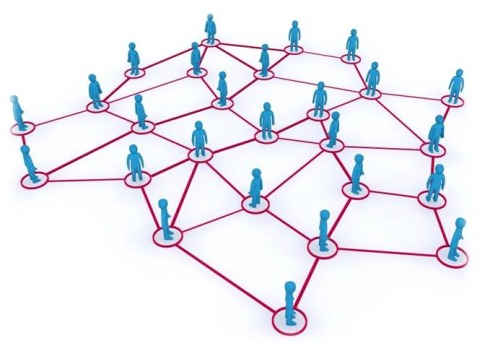
\includegraphics[width=0.75\textwidth]{figures/fig2-1}
  \caption{一个简单的社交网络抽象图}\label{fig:fig2-1}
\end{figure}

\subsection{社交网络的统计特性}
因为社交网络的本质其实就是一个由节点(人或组织)和边(社会关系)组成的图结构,所以社交网络模型之中的很多概念都来源于图论。在这一小节中,将会简单介绍社交网络中常用的几种统计概念,包括节点的度、网络密度、平均路径长度、边的介数和聚类系数。这些统计概念或多或少都旨在反映社交网络的一些特性,比如疏密程度、信息传播开销等等。

(1)节点的度(Degree)

在无向图中,任意节点的度即是与其相连的边的数目。而在有向图中,又可以细分为入度和出度,即分别以节点为终点和起点的边的数目。在社交网络之中,一个节点的度越大,就表示其在这个网络中扮演着越重要的角色。影响力越大的人,在网络中节点的度就越大。例如在微博上,明星拥有着众多的粉丝,而普通用户往往只有很少的粉丝,前者在社交网络中抽象成的节点的度就会很大,后者的度就会很小。网络的平均节点度就是网络中所有节点的度的平均值,它可以反映网络的疏密程度。此外,还可以通过节点度的分布来刻画描述不同节点的重要性。

(2)网络密度(Density)

在社交网络之中,网络密度被定义为网络中实际存在的边数与最多可容纳边数的比值。通常被用来测量社交网络中社交关系的紧密程度及其演变趋势,其计算方式可参考公式\ref{eqn:density}。如果一个社交网络的网络密度比较小,则说明该网络还尚且处在起步阶段;而若一个社交网络的网络密度比较大,那么说明该网络已经比较成熟,网络之中几乎所有节点之间都有联系。

\begin{equation}
  \label{eqn:density}
  Density=\frac{2m}{n(n-1))} 
\end{equation}

公式\ref{eqn:density}中的n和m分别为社交网络中节点的数目和边的数目,且$Density\in [0,1]$。其中,当整个网络中没有一条边,即所有节点都独立存在时,$Density$取0;而当网络中所有节点之间都有边相连时,即网络处于全连接状态时,$Density$取1。一般而言,大规模的社交网络的密度会比中小规模的小一些,因此,不同规模社交网络之间的网络密度也就不具有可比性了。例如,分别以学校和家庭为规模建立一个社交关系网络,显然一个家庭关系的网络密度会大很多。

(3)平均路径长度(Average Path Length)

一个社交网络的平均路径长度被定义为:所有联通节点之间最短路径的平均值。即所有节点之间的最短路径上存在的节点个数的平均值。其计算方法可参考公式\ref{eqn:APL}。

\begin{equation}
  \label{eqn:APL}
  APL=\frac{2}{n(n-1)}\sum _{i=1}^{n}\sum_{j=1}^{n}d_{ij}
\end{equation}

公式\ref{eqn:APL}中的n为当前网络中节点的数目,$d_{ij}$为网络中节点$v_i$和$v_j$之间的最短路径。平均路径长度$APL$通常也是用于反映网络间的紧密程度的,一般也可叫做网络的平均距离。如果社交网络的平均路径长度比较大,则代表网络比较稀疏,节点之间进行信息传播的开销比较大;相反,若社交网络的平均路径长度小,则代表网络稠密,节点之间可以比较迅速快捷的进行消息传递。

(4)聚类系数(Clustering Coefficient)

根据图论,聚类系数表示的是一个图中节点汇聚程度的系数。在很多社交网络中,若节点$v_i$与节点$v_j$相连接,而节点$v_j$与节点$v_k$相连接,那么很大概率上节点$v_i$和节点$v_k$也会相连。这种现象也表明了社交网络中部分节点之间存在着密集连接的这一特性。在无向图中,节点$v_j$的聚类系数$CC_{v_j}$的计算方式可参考公式\ref{eqn:CC}。

\begin{equation}
  \label{eqn:CC}
  CC_{v_j}=\frac{n}{C_k^2}=\frac{2n}{k(k-1)}
\end{equation}

公式\ref{eqn:CC}中$k$表示节点$v_j$所拥有的邻居节点的数目,n表示节点$v_j$的所有相邻节点之间互相连接的边的数目。简而言之,聚类系数可以用来描绘社交网络中一个用户的朋友们之间也是朋友的概率,反映的也就是社交网络的聚集性。具体的,它还可以分为全局聚类系数和局部聚类系数。

(5)介数(Betweeness)

介数可以分为节点介数和边介数,表示的是网络图中某一节点或者某一条边被整个图中所有节点间的最短路径经过的概率之和。通常被用来评价节点的重要程度。在连接不同社区之间的中间节点(或者边)的介数就会比其他节点(或者边)的介数要大很多,这也反映了这类节点在社交平台中作为消息传播的核心地位及其重要程度。对于网络中任意节点v,其介数的计算方式可参考公式\ref{eqn:bet}。

\begin{equation}
  \label{eqn:bet}
  C_B(v)=\sum _{s\neq v\neq t \in V}\frac{\sigma_{st}(v)}{\sigma_{st}}
\end{equation}

在公式\ref{eqn:bet}中,$\sigma_{st}(v)$表示经过节点$v$的$s\rightarrow t$的最短路径条数,$\sigma_{st}$表示$s\rightarrow t$的最短路径条数。直观上来看,节点$v$的介数$C_B(v)$反映的是节点$v$作为“桥梁”或者“枢纽”的重要程度。

\subsection{社交网络的典型特征}
在社交网络之中普遍存在着两个典型的特征:小世界效应和无标度特性。

(1)小世界效应

1929年匈牙利作家F.Karinthy率先提出了“小世界现象(Small-world Effect)”的论断。他认为,平均而言地球上的任何两个人都可以通过一条由5位联系人组成的链条而联系起来。在1967年,美国哈佛大学的社会心理学教授Stanley Milgram提出了著名的“六度分隔(Six Degrees of Separation)假说”\cite{Milgram1967The},大意同样为任何两个想要取得联系的陌生人之间最多只隔着5个人,便可完成两人之间的联系。他通过设计了一个信件实验来证明他的猜想,实验大致经过为:他随机选择了300余人,每人分发一封信并指定各不相同的收信者;要求如果寄信者认识收信者,则直接寄出,否则就寄给一个自己认识的并且可能认识收信者的人,直至收信者收到信为止;实验最终共有约60人收到了信,而这些信平均经手了6次就到达了收信人手中。在1998年的时候,Duncan Watts和Steven Strogatz正式提出了小世界网络的概念并建立了小世界模型\cite{Watts1998Collectivedynamics}。文献中将具有“小世界效应”的网络定义为:网络中任意两个节点之间的平均距离(即平均路径长度APL)随网络中节点数n的增加呈对数增长,即$APL\sim ln(n)$,且网络的局部结构上仍然具有较明显的集团化特征。

小世界效应反映的是社交网络中任何用户之间都近在咫尺的现象,即:社交网络的平均路径长度都很短。小世界现象在在线社交网络中得到了很好地验证,根据2011年Facebook数据分析小组的报告,Facebook约7.2亿用户中任意两个用户间的平均路径长度仅为4.74,而这一指标在Twitter中为4.67。因此可以说,在五步之内,任何两个网络上的个体都可以互相连接。

(2)无标度特性

大多数社交网络都存在着少数节点的度极大,而大部分节点都只有较小的度这一现象。网络因为缺乏一个统一的衡量尺度而呈现出异质性,这种节点度分布不存在有限衡量分布范围的性质就被称为无标度。这其实体现的是社交网络中用户的度呈现出幂律分布(Power-law Distribution)的规律。幂律分布广泛存在于各个领域,其核心就是绝大部分事件的规模其实很小,但是极少数事件的规模却表现的相当大。例如:世界上绝大部分的财富都被掌握在极少数的超级富豪的手中;以网站的访问量而言,尽管互联网上为广大网民提供了无数的网页,但是大家每天访问量最多的仅仅就是几个熟悉的网页;在微博上,一个明星的粉丝可能有上百万乃至上千万,但是大部分普通人也只有寥寥无几的粉丝关注量。在直观上,这个现象就像图\ref{fig:fig2-2}中幂函数曲线一样。幂律分布其实体现的是一种极端的不平衡性。

\begin{figure}
  \centering
  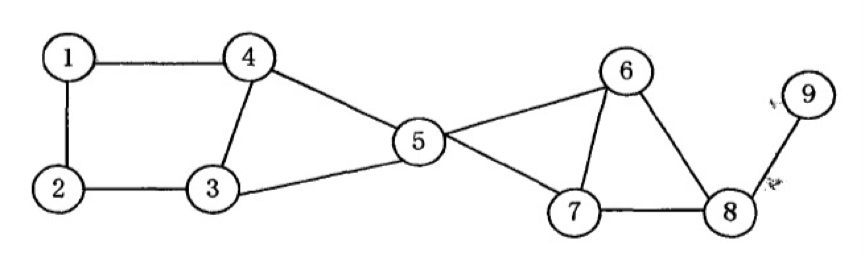
\includegraphics[width=0.75\textwidth]{figures/fig2-2}
  \caption{社交网络中度的幂律分布曲线}\label{fig:fig2-2}
\end{figure}

\section{社区发现}
\subsection{社区的定义}
社交网络除了小世界效应和无标度特性这两个典型特征之外,还有一个重要的一个特点就是“社区(Community)”的存在。也有部分学者将之译为“社团”,本文将之称为社区。在直观上,同现实生活中所说的社区一样,社交网络乃至复杂网络中的社区也可以简单地被理解为是一些彼此之间联系紧密的节点的集合,或者说是一些拥有共同或相似属性的个体组成的团体,这些集合或者团体对于分析社交网络有着至关重要的意义。目前在学术界对社区的概念尚且还没有一个完整统一的定义。本文下面从不同的角度给出了三种定义:基于网络拓扑结构的定义、基于节点相似度的定义和重叠社区的定义。

(1)基于网络拓扑结构的社区定义

将社交网络抽象成一个由节点(人或组织)和边(社会关系)组成的网络拓扑结构,那么一个社区即是指由若干个节点组成的具有高内聚特性的子集合。在这个子集合之中的节点彼此之间联系紧密,表现上就是子集内部节点之间存在着相对比较多的边;而在多个子集合之间,也就是社区之间联系比较稀疏,表现上就是存在着相对较少的边。图\ref{fig:fig2-3}所示即是一个具有社区结构的网络。图中的14个节点组成的网络拓扑图中形成了3个社区结构,为了更直观显示,三个社区的节点分别以黄色、蓝色和绿色三种颜色区分。此种定义对应的社区发现算法即是本文绪论第二小节国内外研究现状中提到的基于链接的社区发现算法。

\begin{figure}
  \centering
  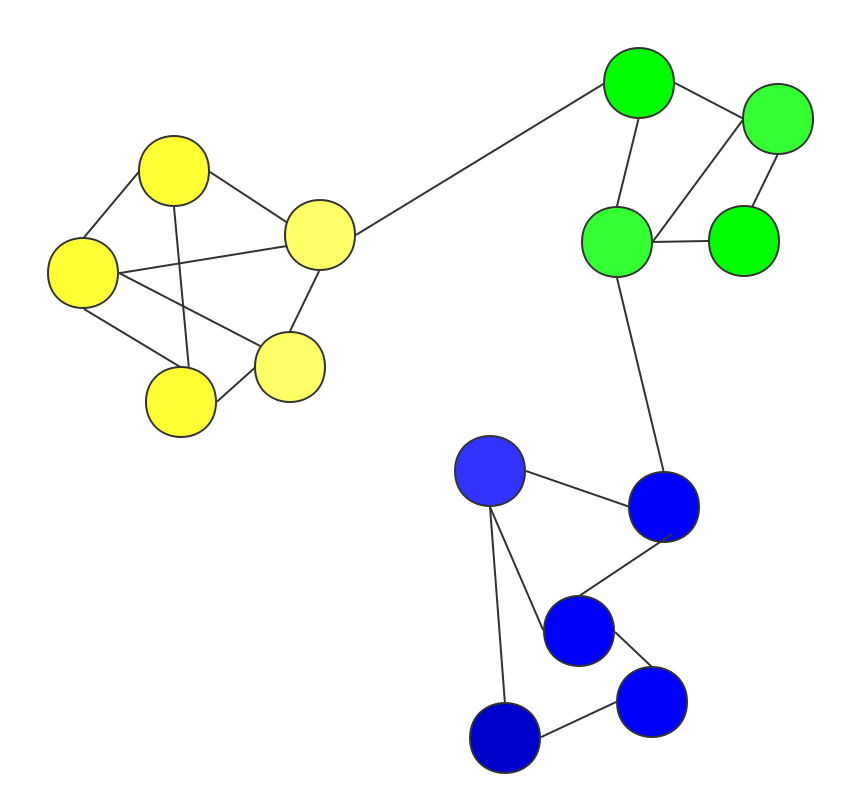
\includegraphics[width=0.75\textwidth]{figures/fig2-3}
  \caption{一个具有社区结构的网络示意图}\label{fig:fig2-3}
\end{figure}

(2)基于节点相似度的社区定义

这里定义的社区依然是由若干节点组成的子集合,但是在表现形式以及定量分析手段方面与上一种定义有所区别。基于节点相似度的社区定义认为属于同一个社区的节点都是相似的,而社区与社区之间的节点的相似度则较低。节点之间的相似度的高低依靠建立节点相似度模型来衡量。该定义相较基于网络拓扑结构的定义会更易于理解,因为社区本就是代表着社交网络中具有相同或者类似属性的元素的子集。此种定义对应的社区发现算法即是本文绪论第二小节国内外研究现状中提到的基于内容的社区发现算法。

其实在本质上,基于网络拓扑结构的社区定义和基于节点相似度的社区定义是一致的。两者都是将社区定义为网络中所有元素组成的集合的若干子集,在子集之中的元素基于某种因素会彼此连接紧密,而与其他子集内的元素连接稀疏。只不过两者对于元素之间的紧密与稀疏的定量分析手段不同,前者是根据网络的拓扑结构和节点之间的边的联系,而后者是根据节点的属性分析节点间相似度。

(3)重叠社区的定义

此前关于社区的定义都忽视了个体可能属于两个或更多社区的可能性。但是,许多真实的社交网络都存在着社区的重叠。例如,一个人可以同时属于家庭群体和朋友群体这两个社交群体。图\ref{fig:fig2-4}所示即是一个具有重叠社区结构的网络。图中的16个节点组成的网络拓扑图中形成了3个社区结构,三个社区的节点分别以黄色、蓝色和绿色三种颜色区分,而这其中有两个黄蓝相间的节点即是同时属于黄色代表的社区和蓝色代表的社区。重叠社区(Overlapping Community)和普通社区相比,唯一的差别就在于:代表重叠社区的子集之间可以有交集,而代表普通社区的子集之间是没有交集的。在包含重叠社区的网络中,这些重叠社区间的交集,即这些属于多个社区的元素(个体),对社区的演化和社区间的沟通都起到了极其重要的作用,因为它们就是不同社区之间的桥梁和纽带。一般而言,重叠社区结构也可以分为两种。一种是离散型重叠社区,即对于一个社区,某个节点只有属于和不属于这两个选择项。另一种是模糊型重叠社区,即每个节点有着对于不同社区的隶属度。关于重叠社区定义对应的社区发现算法即是本文绪论第二小节国内外研究现状中提到的重叠社区发现算法。

\begin{figure}
  \centering
  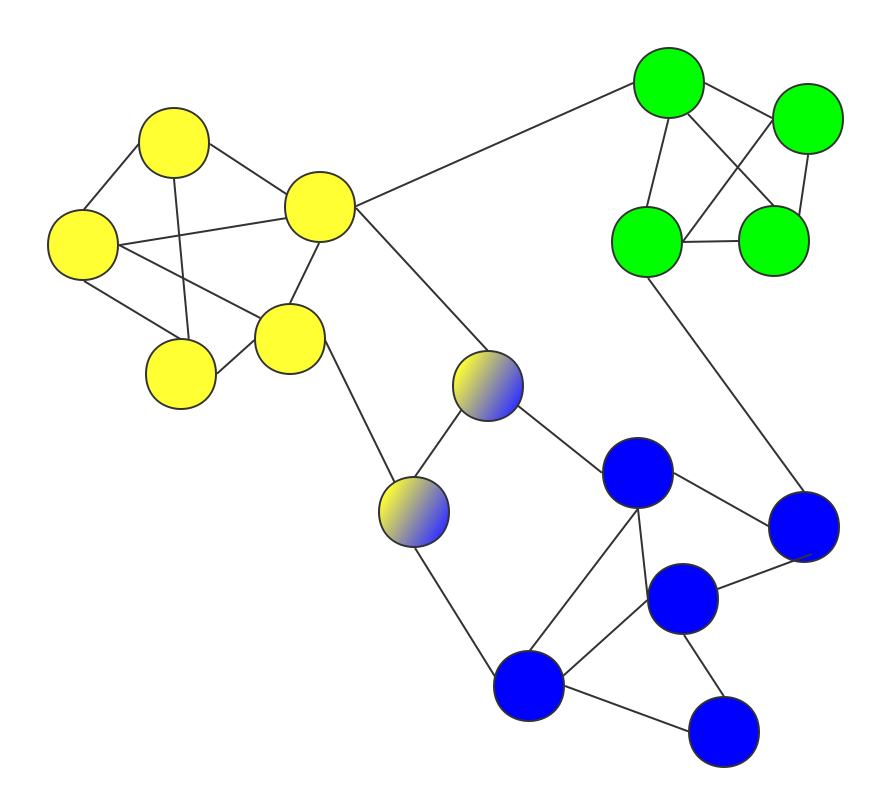
\includegraphics[width=0.75\textwidth]{figures/fig2-4}
  \caption{一个具有重叠社区的网络示意图}\label{fig:fig2-4}
\end{figure}

\subsection{社区发现概述}
上一小节已经较为详细的解释了社区的含义。那么给定一个网络图$G=(V,E)$,其中顶点集为$V$,边集为$E$,社区发现(Community Detection,也可以译作社区检测或者社团检测)即是在网络之中发现社区结构的过程。挖掘社交网络中的社区在人物分析、商业个性化推荐和舆情控制等领域均有着很关键的作用。

在社交网络之中,社区结构是客观存在的,但是往往人们只会与他们有直接接触的用户进行互动,而在同一个社区中,还存在着不少与他有着共性的用户,很可能他们有着共同的朋友但彼此之间却不了解,因此如果要进行朋友推荐,那么隶属于同一社区的成员之间就应该率先进行彼此推荐。此外,对一个大型网络调用社区发现算法,其实是对其按照某种标准进行了划分,在此基础上可对每个社区做进一步的挖掘。而从计算的角度而言,社区划分相当于分解了任务,起到了降低计算复杂度的作用。并且目前的社交软件上用户广泛,无法将所有用户的信息都存储在同一台服务器之上,这就必须要使用到分布式存储。在分布式存储中,如果不经过分类杂乱无章的进行存储,那么最终将导致巨大的通信开销,而如若先将社交网络进行社区发现,把同一社区内的用户存储在同一服务器内,这就可以省下大笔的通信开销,大大提高社交平台的性能。

近年来,对社交网络中的社区结构进行检测并分析已经吸引了众多研究人员的关注,一大批社区发现算法也随之被提出。在本文绪论第二小节国内外研究现状中将社区发现算法分为了基于链接的算法、基于内容的算法和融合了链接与内容的算法。对于社区的重叠问题,还可以将社区发现分为非重叠和重叠的社区发现,在本文的国内外研究现状中也有对重叠社区发现算法进行了简单的综述。因此,对于具体的社区发现算法,此处不再赘述。

\section{本章小结}
本章主要是对社交网络以及社区发现的相关概念进行了综述。首先给出了社交网络在维基百科中的定义,在此基础上对社交网络这一概念进行了简单的描述;其次对社交网络的五大重要的统计特性以及两大典型特征进行了一一说明;接着从三个不同角度对社区的定义进行了详细介绍,最后引出了社区发现这一概念,并对其进行了必要的介绍。




%%==================================================
%% chapter03.tex for BIT Master Thesis
%% modified by 朱杰
%%==================================================
\chapter{基于稳定标签传播的非重叠社区发现算法}

由于社交网络“小世界”、“无标度”的特性以及目前社交网络普遍具有大规模的数据量,这对算法的时间复杂度提出了严格的要求。尽管至今已有为数不少的社区发现算法被学者们相继提出,但是这些算法大多是在社区识别的准确率上进行不断创新和优化,针对的多是中小规模的网络,面对大规模的社交网络数据这些算法往往需要巨大的时间开销。而本文在第一章节国内外研究现状中也已经提到,标签传播算法(LPA算法)\cite{Raghavan2007Near}是目前算法时间复杂度最低的社区发现算法,算法简单易理解且不需要任何先验信息,但是标签传播算法也有些许问题,例如稳定性差和算法无法收敛等。
% 截至今天已经有不少学者在LPA算法的基础上进行了改进和创新,例如Leung等人\cite{Leung2009Towards}引入了启发式思想,在节点属性中加上了创新提出的hop score值,以此来提高算法效率及性能;文献\cite{He2014A}则是修改了LPA算法迭代的终止条件;LabelRank算法\cite{Xie2013LabelRank}创新的提出了标签概率矩阵,此法解决了LPA算法运行结果不稳定的问题。

标签传播算法是最早的基于标签传播思想的非重叠社区发现算法,本章节基于该算法进行研究和改进,将提出一种稳定的基于标签传播的非重叠社区发现算法(Community Detection Algorithm Based on Stable Label Propagation),下文简称CDABSLP算法。

CDABSLP算法通过采用异步标签更新的策略来避免LPA算法标签传播过程中可能产生震荡的问题;在节点迭代更新标签时将节点按照节点的重要性降序排列,而非原始的随机顺序;在设计节点重要性评价指标上引进了k-核分解方法,设计了一个全新的综合节点自身影响力以及邻居节点影响力的节点影响力模型;在标签选择方式上同样进行相应的改进,针对出现多个最多邻居标签的情况,在节点影响力模型的基础上设计了标签影响力模型,选取标签影响力最大的标签进行更新。在这一系列改进之后,使得标签传播过程更加稳定,收敛速度快速。

本章接下来的内容组织结构上将先介绍一下标签传播算法的情况,详细分析LPA算法目前存在的缺陷;然后详细的阐述CDABSLP算法在使得标签传播更加稳定性上的设计;接着是对算法整体执行步骤进行全面的说明,并对算法时间复杂度进行分析;最后在验证实验部分中,介绍了包括实验环境、实验数据集以及评价指标后,将会详细的分析在真实网络以及人工基准网络上的实验结果,通过与其他基准算法进行对比实验,以此来证明算法的效果。

\section{标签传播算法的缺陷分析}

标签传播算法早在2002年就被Zhu等人\cite{Zhu2002Learning}提出,这是一种基于图的半监督机器学习算法,它的基本思想是用已经标记的节点的标签信息来预测未标记节点的标签信息。如本文在第一章节国内外研究现状中提及的,是Raghavan等人\cite{Raghavan2007Near}于2007年第一次将LPA算法应用于社区发现领域。LPA算法的主要思想就是利用复杂网络固有的拓扑结构中隐藏的信息来引导探测出网络中存在的“社区”。在起始的时刻,LPA算法会为网络中所有的节点分配一个独一无二的标签,通常就是节点的ID,这代表所有的节点都是单独的一个社区;然后就是不断迭代着更新所有节点的标签,直至收敛,即不再有标签发生改变为止;在每一轮更新标签的过程中,每个节点会将自己的标签修改为自己邻居节点中出现次数最多的那个标签,当出现多个邻居节点的标签均为最大出现数时,随机选择其中一个标签进行更新。在整个重复迭代更新标签的过程中,联系密切的节点最终会被标记为同样的标签,这样在标签传播结束之后,LPA算法可以按照节点不同的标签将节点进行社区划分。

图\ref{fig:dingdianbiaoqianchuanbo}展示了网络中一个节点获取标签的过程。图中的灰色节点在更新其标签时,它拥有的5个邻居节点之中有三个邻居节点标签为为黑色,而两个邻居节点为白色,故将其节点更新为黑色。

\begin{figure}
  \centering
  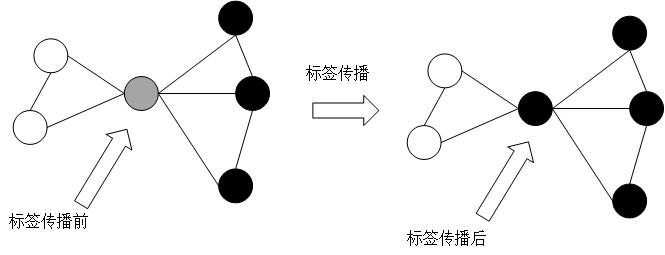
\includegraphics[width=0.75\textwidth]{figures/dingdianbiaoqianchuanbo}
  \caption{节点获取标签的示例图}\label{fig:dingdianbiaoqianchuanbo}
 \end{figure}

公式\ref{eqn:biaoqiangengxin}为标签传播算法中节点更新标签的公式。

\begin{equation}
  \label{eqn:biaoqiangengxin}
  c_i=\arg\max_l \left | \Gamma _i^l \right |
\end{equation}

其中$\Gamma _i^l$表示的是具有标签$l$的节点$i$的邻接节点集合。

标签传播算法执行步骤的具体实现伪代码可参考算法\ref{alg:LPA}。

\begin{algorithm}[htb]  
  \caption{标签传播算法(LPA)}  
  \label{alg:LPA}  
  \begin{algorithmic}[1]  
    \Require
      社交网络$G=(V,E)$,节点总数$N$,最大允许迭代轮数$maxIter$,停止迭代标签修改率$stopIterRatio$;  
    \Ensure  
      网络中所有的社区及其成员;  
    \State  初始化阶段:

    (a)标签初始化:为所有节点设置初始标签,设为其节点ID即可;

    (b)迭代次数初始化:迭代次数$iter = 0$;

    (c)标签改变数初始化:标签改变数量$changedNum = 0$

    \State  标签传播阶段:
      
    (a)如果迭代次数$iter > maxIter$,停止标签传播,转步骤3;否则继续算法;
    
    (b)将网络中的节点按照随机顺序加入待更新标签队列;
    
    (c)针对队列中的每个节点,遍历其邻居节点,选择邻居节点中出现次数最多的标签,将自身标签更新为该标签;若最大出现次数标签存在多个,则随机选择其中一个即可;
    
    $//$注意此处在邻居节点的标签选择上需要说明的是:在第$iter$轮迭代中,无论邻居节点是否已经在本轮迭代中更新过标签,选择的都是邻居节点第$(iter - 1)$轮中的标签;该更新策略称为同步更新;
    
    (d)若节点标签进行了修改,标签改变数量$changedNum + 1$;
    
    (e)每轮标签传播迭代完毕,检查标签修改比例$\frac{changedNum}{N}$;若$\frac{changedNum}{N} < stopIterRatio$,则停止标签传播,转步骤3;反之令$(iter = iter+ 1)$,转步骤2,继续下一轮迭代;
    \State  社区划分阶段:将具有相同标签的节点划分为一个社区,整个网络中存在的标签数量即是发现的社区数量。
  \end{algorithmic}  
\end{algorithm} 

标签传播是通过相邻节点之间标签的传递来实现社区的划分的,其能够实现较好划分效果的原因是:在社交网络这种特殊的结构之中,节点之间通过边相连通,边本身就代表着节点间的联系,那么就不难理解,节点之间相邻这一事件本身就说明着在某种意义上它们是具有某种相似的属性的,这在标签传播中表现即是相邻的节点理应拥有相同的标签;而如果某个节点集合中各节点之间都有着复杂的关联,或者说它们在某种属性上可以被划分到同一类别,那么在网络中的表现也就是存在着大量的边在这些节点之间,在标签传播的结果上这些节点也就应当有着相同的标签,这实质上也就是达到了聚类的效果。概括来说,正是因为社交网络自身的结构特性,它能直观地表现各个实体之间的关联以及实体的分布规律。

LPA算法虽然简洁明了易实现,但是也存在着一些缺陷使得算法实验结果很不稳定。下面进行简单分析:

首先,LPA算法无法保证算法必然收敛。就以算法\ref{alg:LPA}中的提到的最大允许迭代轮数$maxIter$和停止迭代标签修改率$stopIterRatio$而言,这两个参数设置的初衷正是因为LPA算法的不稳定,无法保证算法必然收敛,若不在迭代次数上进行限制,甚至会陷入无限死循环;例如:在含有二分结构的网络之中进行标签传播存在着标签来回更替而进入“死循环”的问题,如图\ref{fig:fig3-1}中所示。

\begin{figure}
  \centering
  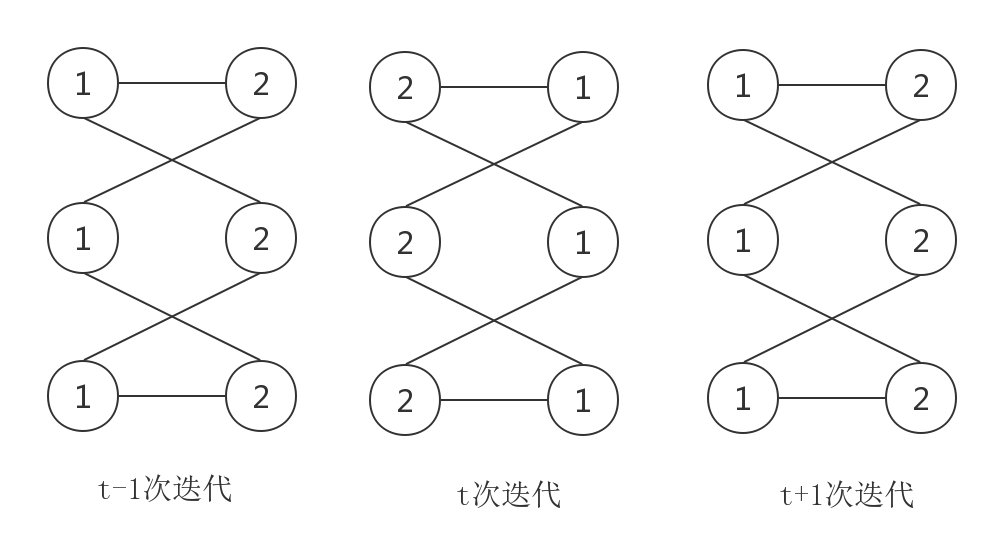
\includegraphics[width=0.75\textwidth]{figures/fig3-1}
  \caption{二分网络中的标签震荡现象}\label{fig:fig3-1}
 \end{figure}

其次,LPA算法第二个不确定性在于其节点更新顺序的随机性。然而很明显的是节点的更新顺序对最终的结果会有很大的影响,且网络之中的不同节点显然是有着不一样的重要程度的。设想一个本来在网络之中起着至关重要作用的节点,如果碰巧被分在最后一个更新标签,那么本轮更新,该节点对其他节点将不会造成任何影响,这显然不是一个很好的选择;即使这对算法的结果没有过多影响,多多少少也会降低算法的收敛速度。最先将重要的节点进行标签更新,显然有助于加快标签的传播。正是在节点更新顺序上的随机性,使得算法存在着不稳定的因素,因此若想要获取稳定的标签传播,在这一方面的改进是必不可少的。

最后,LPA算法第三个不确定性在于其标签选择上随机性。正如算法\ref{alg:LPA}中描述的,当最多出现次数的标签存在多个的时候,随机选择其中一个进行标签更新。很显然当出现多个最大标签时,应该选择的是对自身影响最大的那一个,而不是简简单单的随机选择一个。当然,这就涉及了一个新的问题:对节点之间相互的影响值该如何考量。

经过上述分析可见,原始的LPA算法的确存在着不少有待改进的地方。无论是节点的更新顺序还是在标签的选择方式上,其中的随机性不仅可能影响了算法的收敛速度,甚至可能导致最后的社区发现结果也不稳定。因此,对标签传播算法稳定性问题的解决显得非常必要。下文将提出一种改进的LPA算法以克服原始LPA算法的不足。

\section{算法核心思想}

\subsection{异步更新标签}

在上一小节中提及了LPA算法实验结果不稳定,准确率较低,尤其是算法收敛速度不稳定,甚至可能无法收敛。而这与其标签更新时采用的同步更新策略有关,这在算法\ref{alg:LPA}中也有提及。为了更好的对比突出异步更新标签的优势,下面先介绍一下同步更新与异步更新的概念。

因为每个节点不可能同时更新它们的节点标签,所以在整个网络之中所有节点在更新标签的时候必然存在着先后顺序。在某个节点更新标签的时候,它的部分邻居节点可能已经在它之前进行过标签更新了,而也有部分邻居节点仍然未更新标签,这样一来在标签选择上就面临了一个问题:对于已经在本轮迭代中更新过标签的邻居节点,该节点是选择最新的标签进行参考还是依旧选择上一轮结果中标签。

标签的同步更新是指在每一轮标签传播过程之中,某个节点在考察其邻居节点标签以更新自身标签的时候,无论邻居节点是否已经经历过本轮迭代,均参考的是邻居节点上一轮标签迭代后的结果;而标签的异步更新则参考的是已知最新的邻居节点标签,即:若邻居节点已经经历过本轮迭代,就参考邻居节点本轮标签更新后的结果,反之则参考邻居节点上一轮的迭代结果。

如图\ref{fig:tongbugengxinshili}中所示,按照节点ID号$\{1,3,5,6,4,2,8,7 \} $的顺序对图中网络进行一轮同步更新,因为同步更新需要上一轮迭代的结果,故无法直接覆盖原标签结果,因此在图中更新后的标签标记在相应节点的外侧。从整个更新过程可见得到的结果依然十分随机,结果甚至很难收敛。并且在具体划分的过程之中,因为同步更新参考的邻居节点标签均为上一轮迭代的结果,因此其实节点的更新顺序在此也显得无所谓。

\begin{figure}
  \centering
  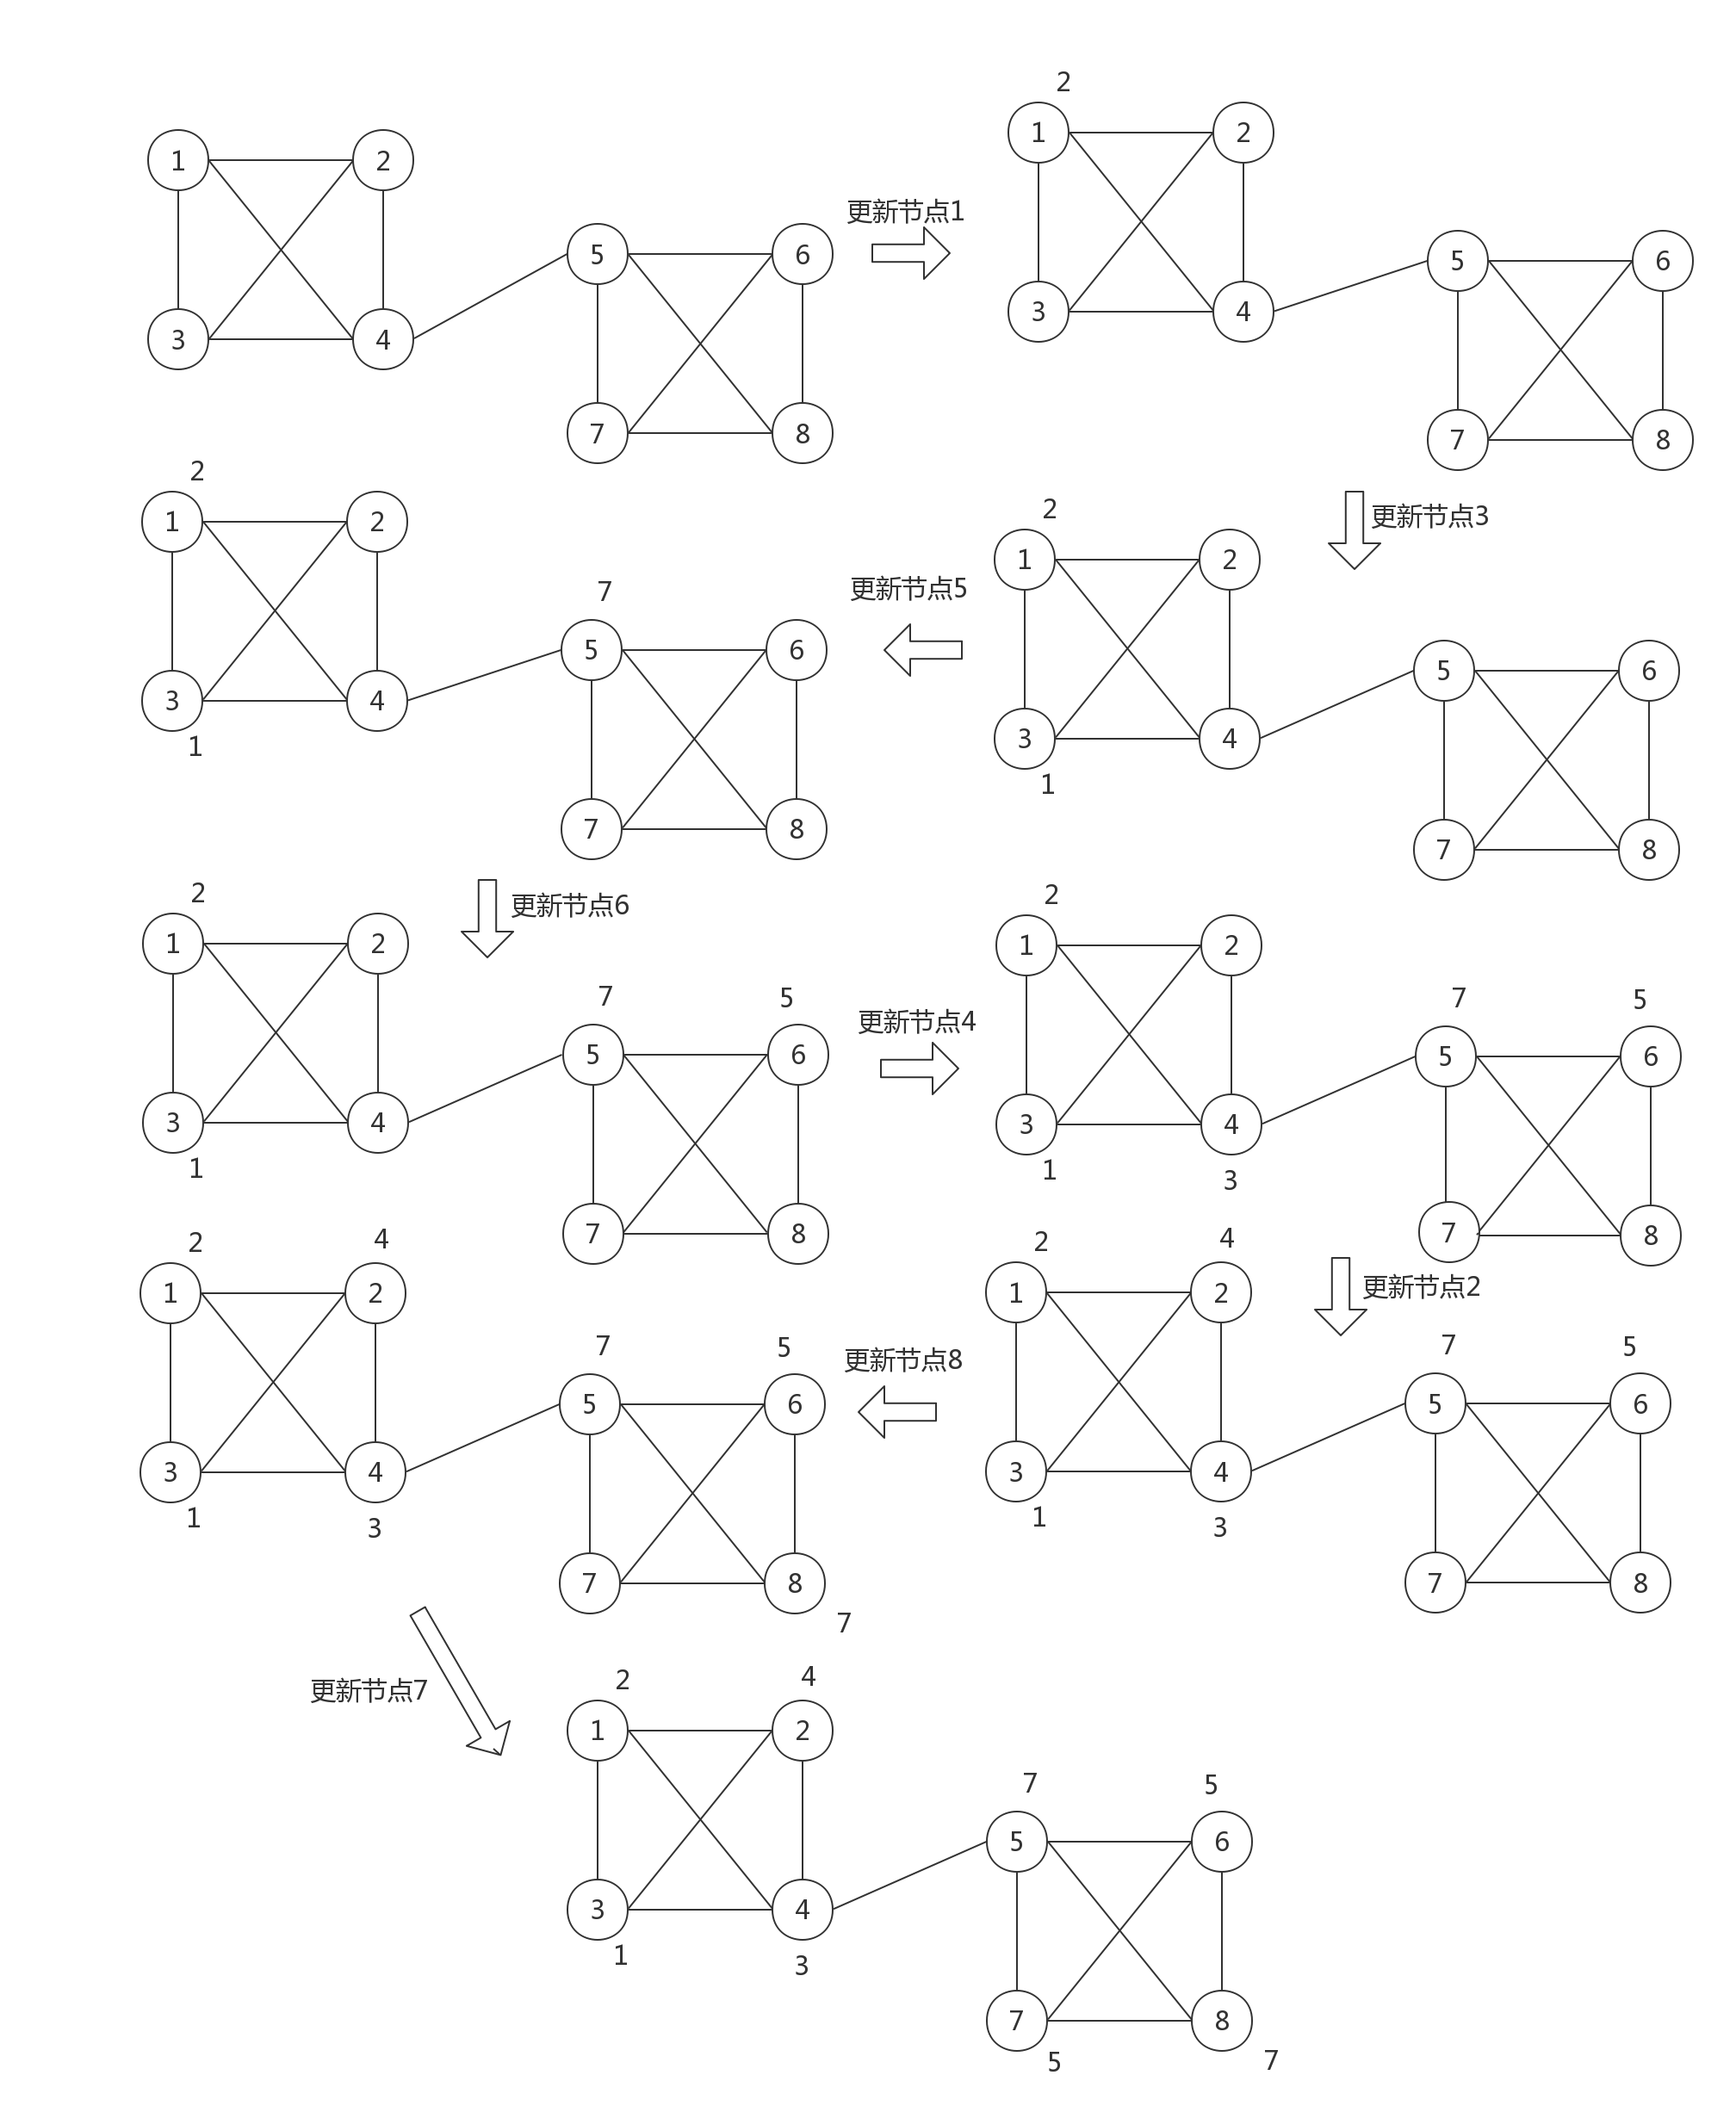
\includegraphics[width=0.95\textwidth]{figures/tongbugengxinshili}
  \caption{标签同步更新示例图}\label{fig:tongbugengxinshili}
\end{figure}

而异步更新则不同,如图\ref{fig:yibugengxinshili}中所示,在示例中按照节点ID号$\{1,3,5,6,4,2,8,7 \} $的顺序对原图中网络进行一轮异步更新,因为无需保存上一轮迭代的结果,故在节点更新标签的时候直接覆盖原标签即可。同样从整个更新过程可见异步的更新过程结果相当令人满意,几乎已经收敛,仅仅只用再多一次迭代就可以获得完整的社区划分。目前标签为“4”的节点在下一轮迭代中也必将被更新为“7”。其他节点均已经在这一轮迭代中被划分到了相应的社区。相比同步更新,显然异步更新的方式更加优秀,不仅能够使得实验结果更加稳定,而且有效地加速了算法的收敛速度。

但是异步更新标签也会对节点的更新顺序以及标签的选择方式提出更高的要求,下面将会介绍本章提出算法在对节点的更新顺序以及标签的选择方式上的改进。

\begin{figure}
  \centering
  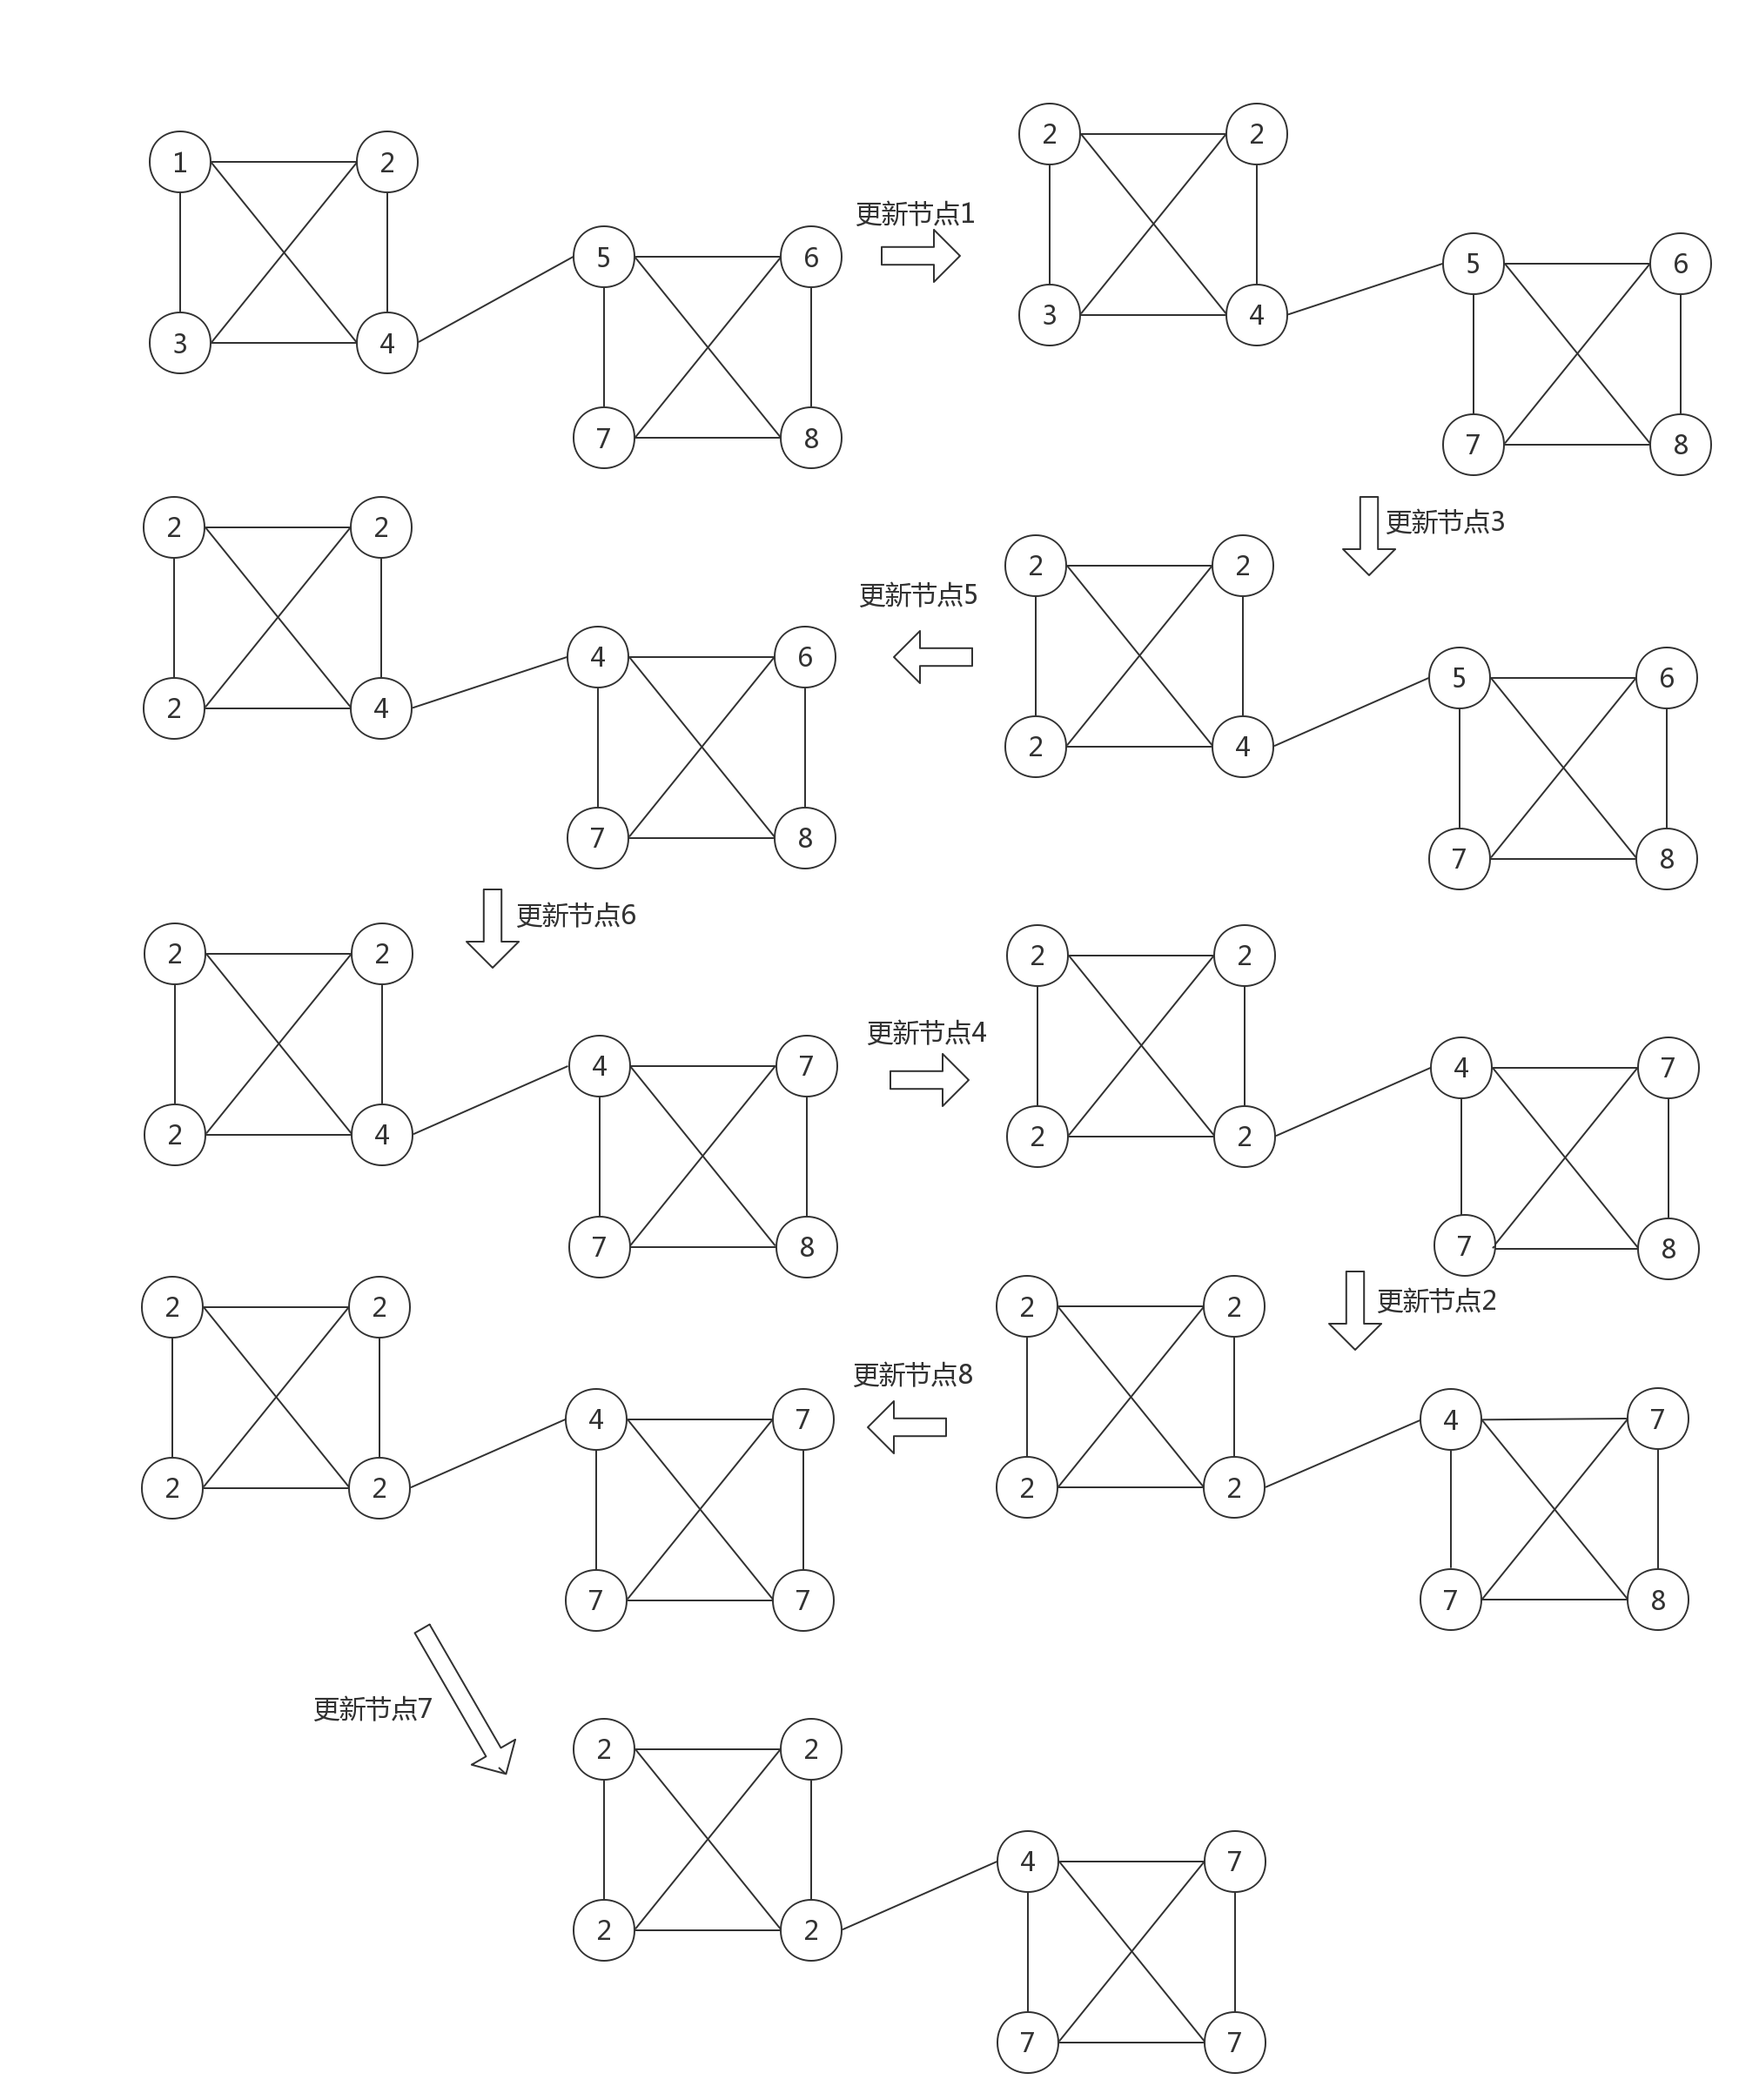
\includegraphics[width=0.95\textwidth]{figures/yibugengxinshili}
  \caption{标签异步更新示例图}\label{fig:yibugengxinshili}
\end{figure}

\subsection{节点更新顺序上的改进}

在采用了异步的标签更新策略之后,虽然使得标签传播更加稳定,也有效地加速了迭代收敛速度,但是异步更新同时也对迭代过程中的节点顺序提出了很高的要求。因为异步更新的缘故,率先进行更新的节点的标签会持续对后续即将更新的节点造成影响,所以如果是社交网络中本就是有着较为重要地位的节点率先进行更新,而社交网络边缘的那些无关紧要的节点最后更新,迭代过程收敛的速度会更快,且最终得到的社区划分也将更为合理。

以一个简洁的网络结构中的异步标签传播过程为例,这是一个5个节点构成的简单网络,如图\ref{fig:jiediansuijigengxinshunxu}中左上角所示。在进行标签传播的过程之中,若按照随机节点顺序进行标签更新,不妨假设按照节点ID号$\{2,1,3,5,4 \} $的顺序进行第一轮标签传播,则可见原始的2号节点率先将其标签更新为它唯一邻居1号节点的标签“1”,然后1号节点自身随机选择了众邻居节点中的一个标签“3”进行了标签更新,最终后续的节点$\{3,5,4 \} $都更新为了标签“3”。这一轮迭代中除了一个节点,其他节点均更新为了统一的标签。在下一轮迭代中,无论如何,标签“1”也会被更新为“3”,最终达到收敛。

\begin{figure}
  \centering
  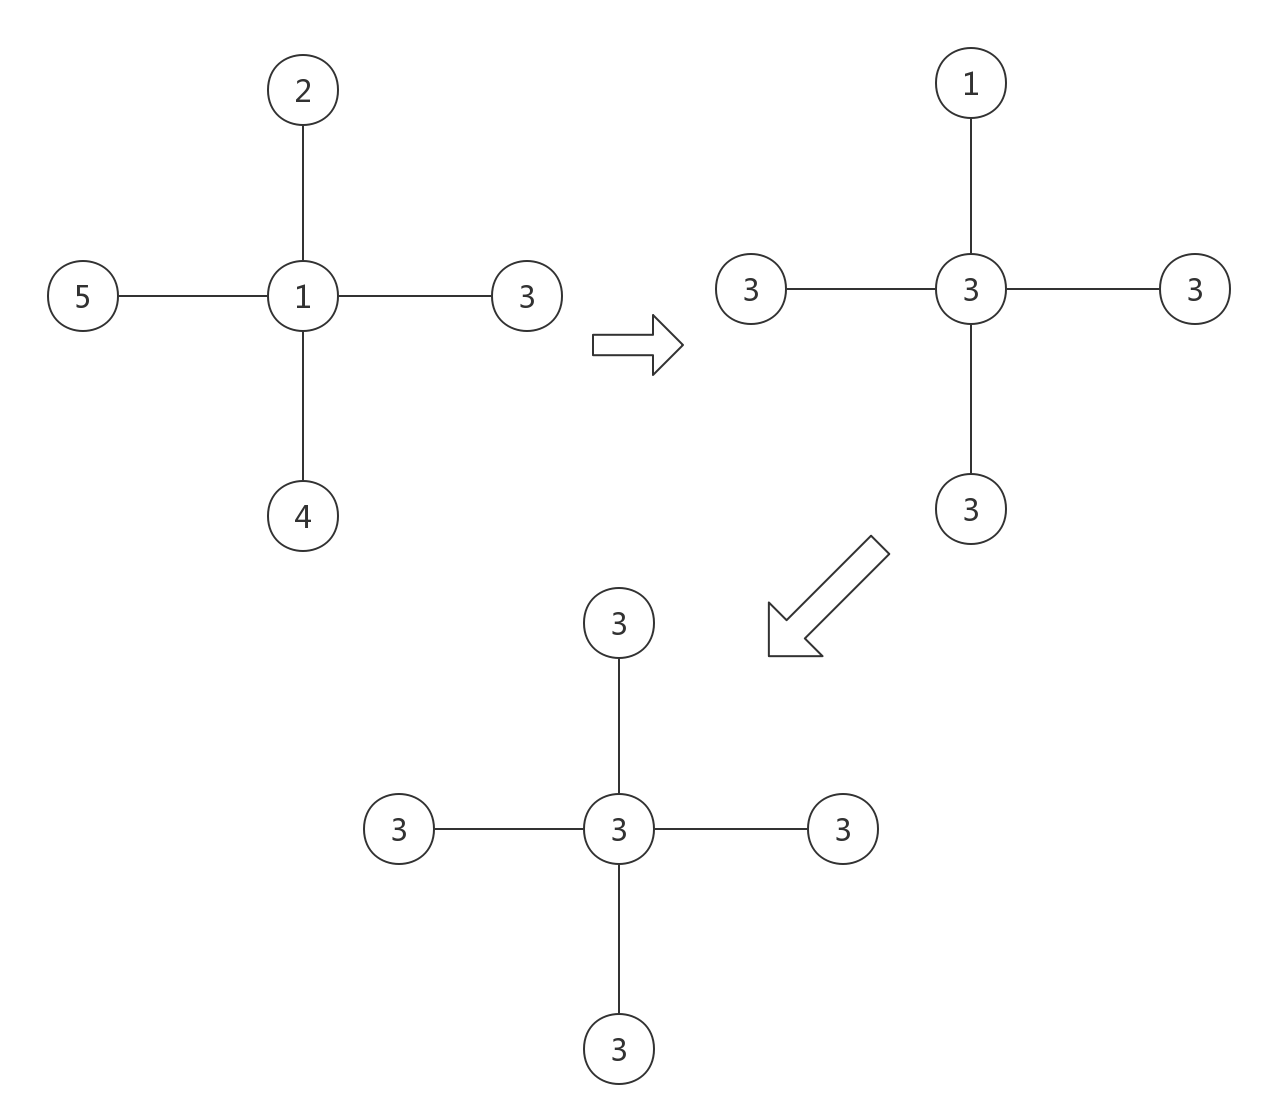
\includegraphics[width=0.75\textwidth]{figures/jiediansuijigengxinshunxu}
  \caption{节点以随机顺序更新的示例图}\label{fig:jiediansuijigengxinshunxu}
\end{figure}

然而在图\ref{fig:jiediansuijigengxinshunxu}中的网络中,很直观地即可看出节点ID号$\{2,3,4 \} $的节点均围绕着1号节点,显然1号节点在这个简单网络结构中具有最重要的地位以及影响度,起着“桥梁”和“枢纽”的作用。如果在节点更新时按照节点的重要性排序来进行更新,那么可想而知那些关键的节点率先更新标签后,可以持续不断地对其他节点的标签更新造成影响。图\ref{fig:jiedianyingxiangzhigengxinshunxu}展示了上述网络中以节点重要性降序排列来进行标签更新的情况。将最重要的1号中心节点率先进行标签更新,而此后其周围节点都会把标签更新为中心节点的标签,在这种情况下仅仅只用了一轮标签迭代后算法就收敛了,相比随机顺序更新少了一轮迭代。而这还仅仅只是在这个简单的示例之中,试想如果是巨大的社交网络,如果按照节点重要性进行排序后再执行标签更新,那么必然会显著地提高算法的收敛速度。

\begin{figure}
  \centering
  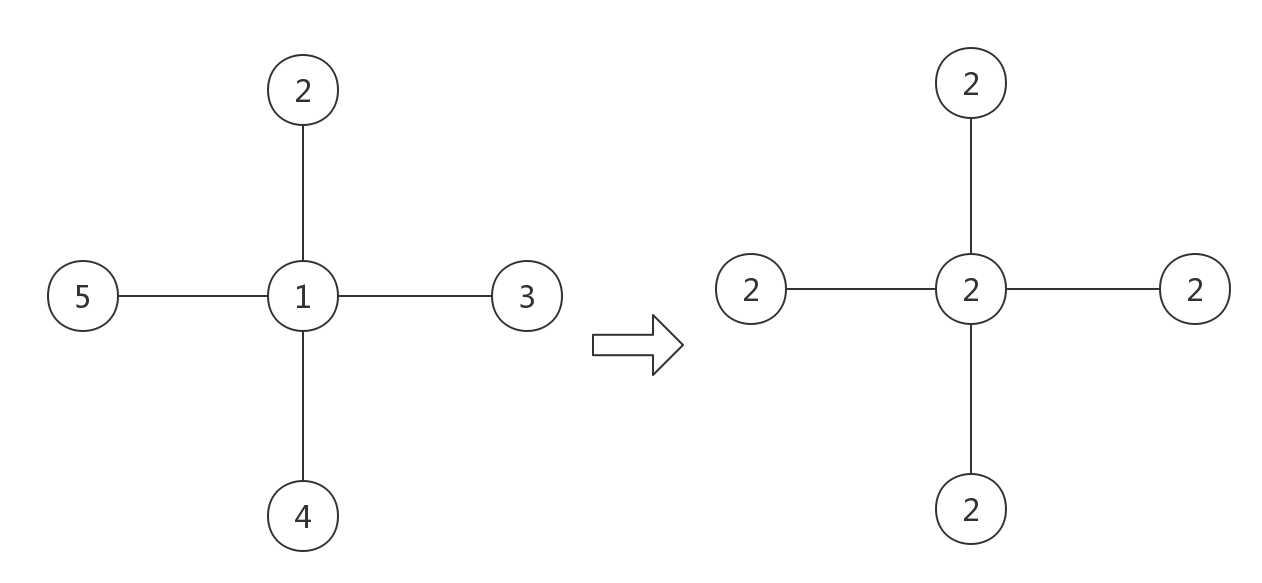
\includegraphics[width=0.75\textwidth]{figures/jiedianyingxiangzhigengxinshunxu}
  \caption{节点以重要性降序更新的示例图}\label{fig:jiedianyingxiangzhigengxinshunxu}
\end{figure}

通过上述分析,本章提出的改进算法将会在第一轮的标签传播之前,先将节点按照节点重要性进行排序,然后在后续的标签传播过程之中,所有的节点按照节点重要性的降序依次更新标签。当然这就涉及了一个新问题,即:如何对节点的重要性进行评判。这一问题的解决方案将会在下一小节中进行详细介绍。

\subsection{节点影响力模型}

在本文第二章研究基础第一小节社交网络的统计特性中,已经提及了多种考量节点重要性或者影响力的统计指标,比如节点的度、聚集系数和介数等等。在这之中,节点的度以及聚类系数虽然均能反应节点在社交网络之中的关键程度,尤其是节点的度因为容易理解且计算方便,不少基于标签传播的改进算法往往会将标签更新顺序直接设置为节点度大小的降序,这样已经能够取得相较原始LPA算法更为出色的效果;但是这两个指标更侧重于社交网络的局部信息,若想要在网络的整体布局上来分析节点的影响力,介数会是一个很好的衡量指标,然而统计网络中所有节点之间的最短路径会消耗巨大的时间,很明显若要对所有节点进行介数的计算,标签传播这一方法仅仅线性时间的执行速度优势将完全不复存在。

而Kitsak等人在文献\cite{Kitsak2010Identification}中提出的k-core分解方法将能很好地解决上述问题,作为一个节点影响力指标。Kitsak等人指出:k-core值高的节点在复杂网络之中具有更强的信息传播能力,即节点的k-core值越高,其影响力越大。

k-核分解方法的核心思路是将整个网络划分为互不相交的多个子网络,在每个子网络中的所有节点在该子网络中的度最小为k。每个节点均有一个k-核值,该值的大小揭示了节点在整个网络中的地位是处在中心位置还是边缘地带,通常可记为$Ks(i)$,表示节点i属于第k-核,但并不属于(k+1)-核。

k-核分解方法的时间复杂度同样只要线性时间,其复杂度为 $O(m)$,$m$为网络中边的总数。通过k-核分解可以分析获取复杂网络的层次性,图\ref{fig:kcoreshili}展示了一个k-核分解的示例,该网络被分解为了三层,此结构就像一个洋葱一样,因此可以很好地反应出网络中的层次性。k-核分解的具体执行步骤可参考算法\ref{alg:k-core},而流程图\ref{fig:k-core}展示了k-核分解法的整个过程。

\begin{algorithm}[h]  
  \caption{k-核分解方法}  
  \label{alg:k-core} 
  \begin{algorithmic}[1]  
    \Require  
      复杂网络$G=(V,E)$;  
    \Ensure  
      k-核划分结果;  
    \State 初始化 $k=0$;  
    \Repeat  
      \State $k = k+1$;
      \Repeat 
        \State 将网络中度小于等于k的节点划分至k-core子集,并删除这些节点以及与这些节点相连的边;
      \Until{网络中不存在度小于等于k的节点}
    \Until{网络中所有节点均已划分完毕}  
  \end{algorithmic}  
\end{algorithm}  

\begin{figure}
  \centering
  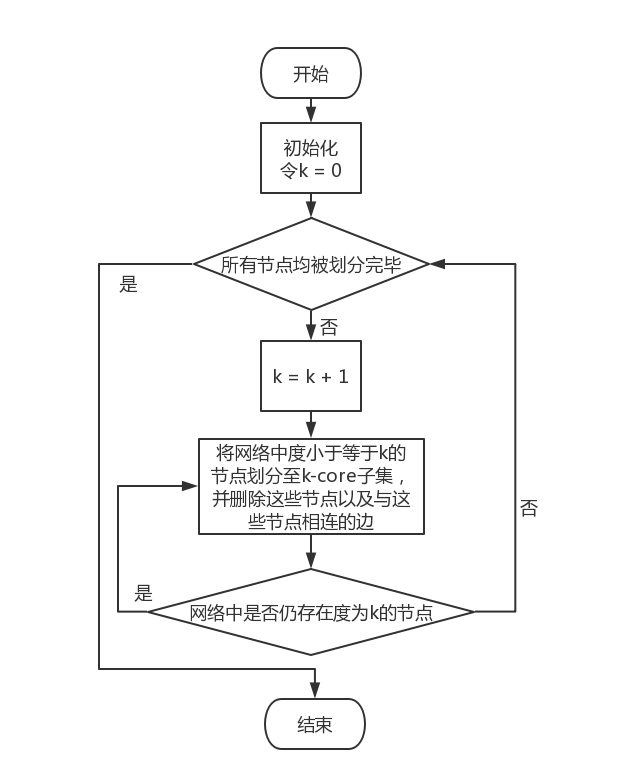
\includegraphics[width=0.75\textwidth]{figures/k-core}
  \caption{k-核分解方法的流程图}\label{fig:k-core}

  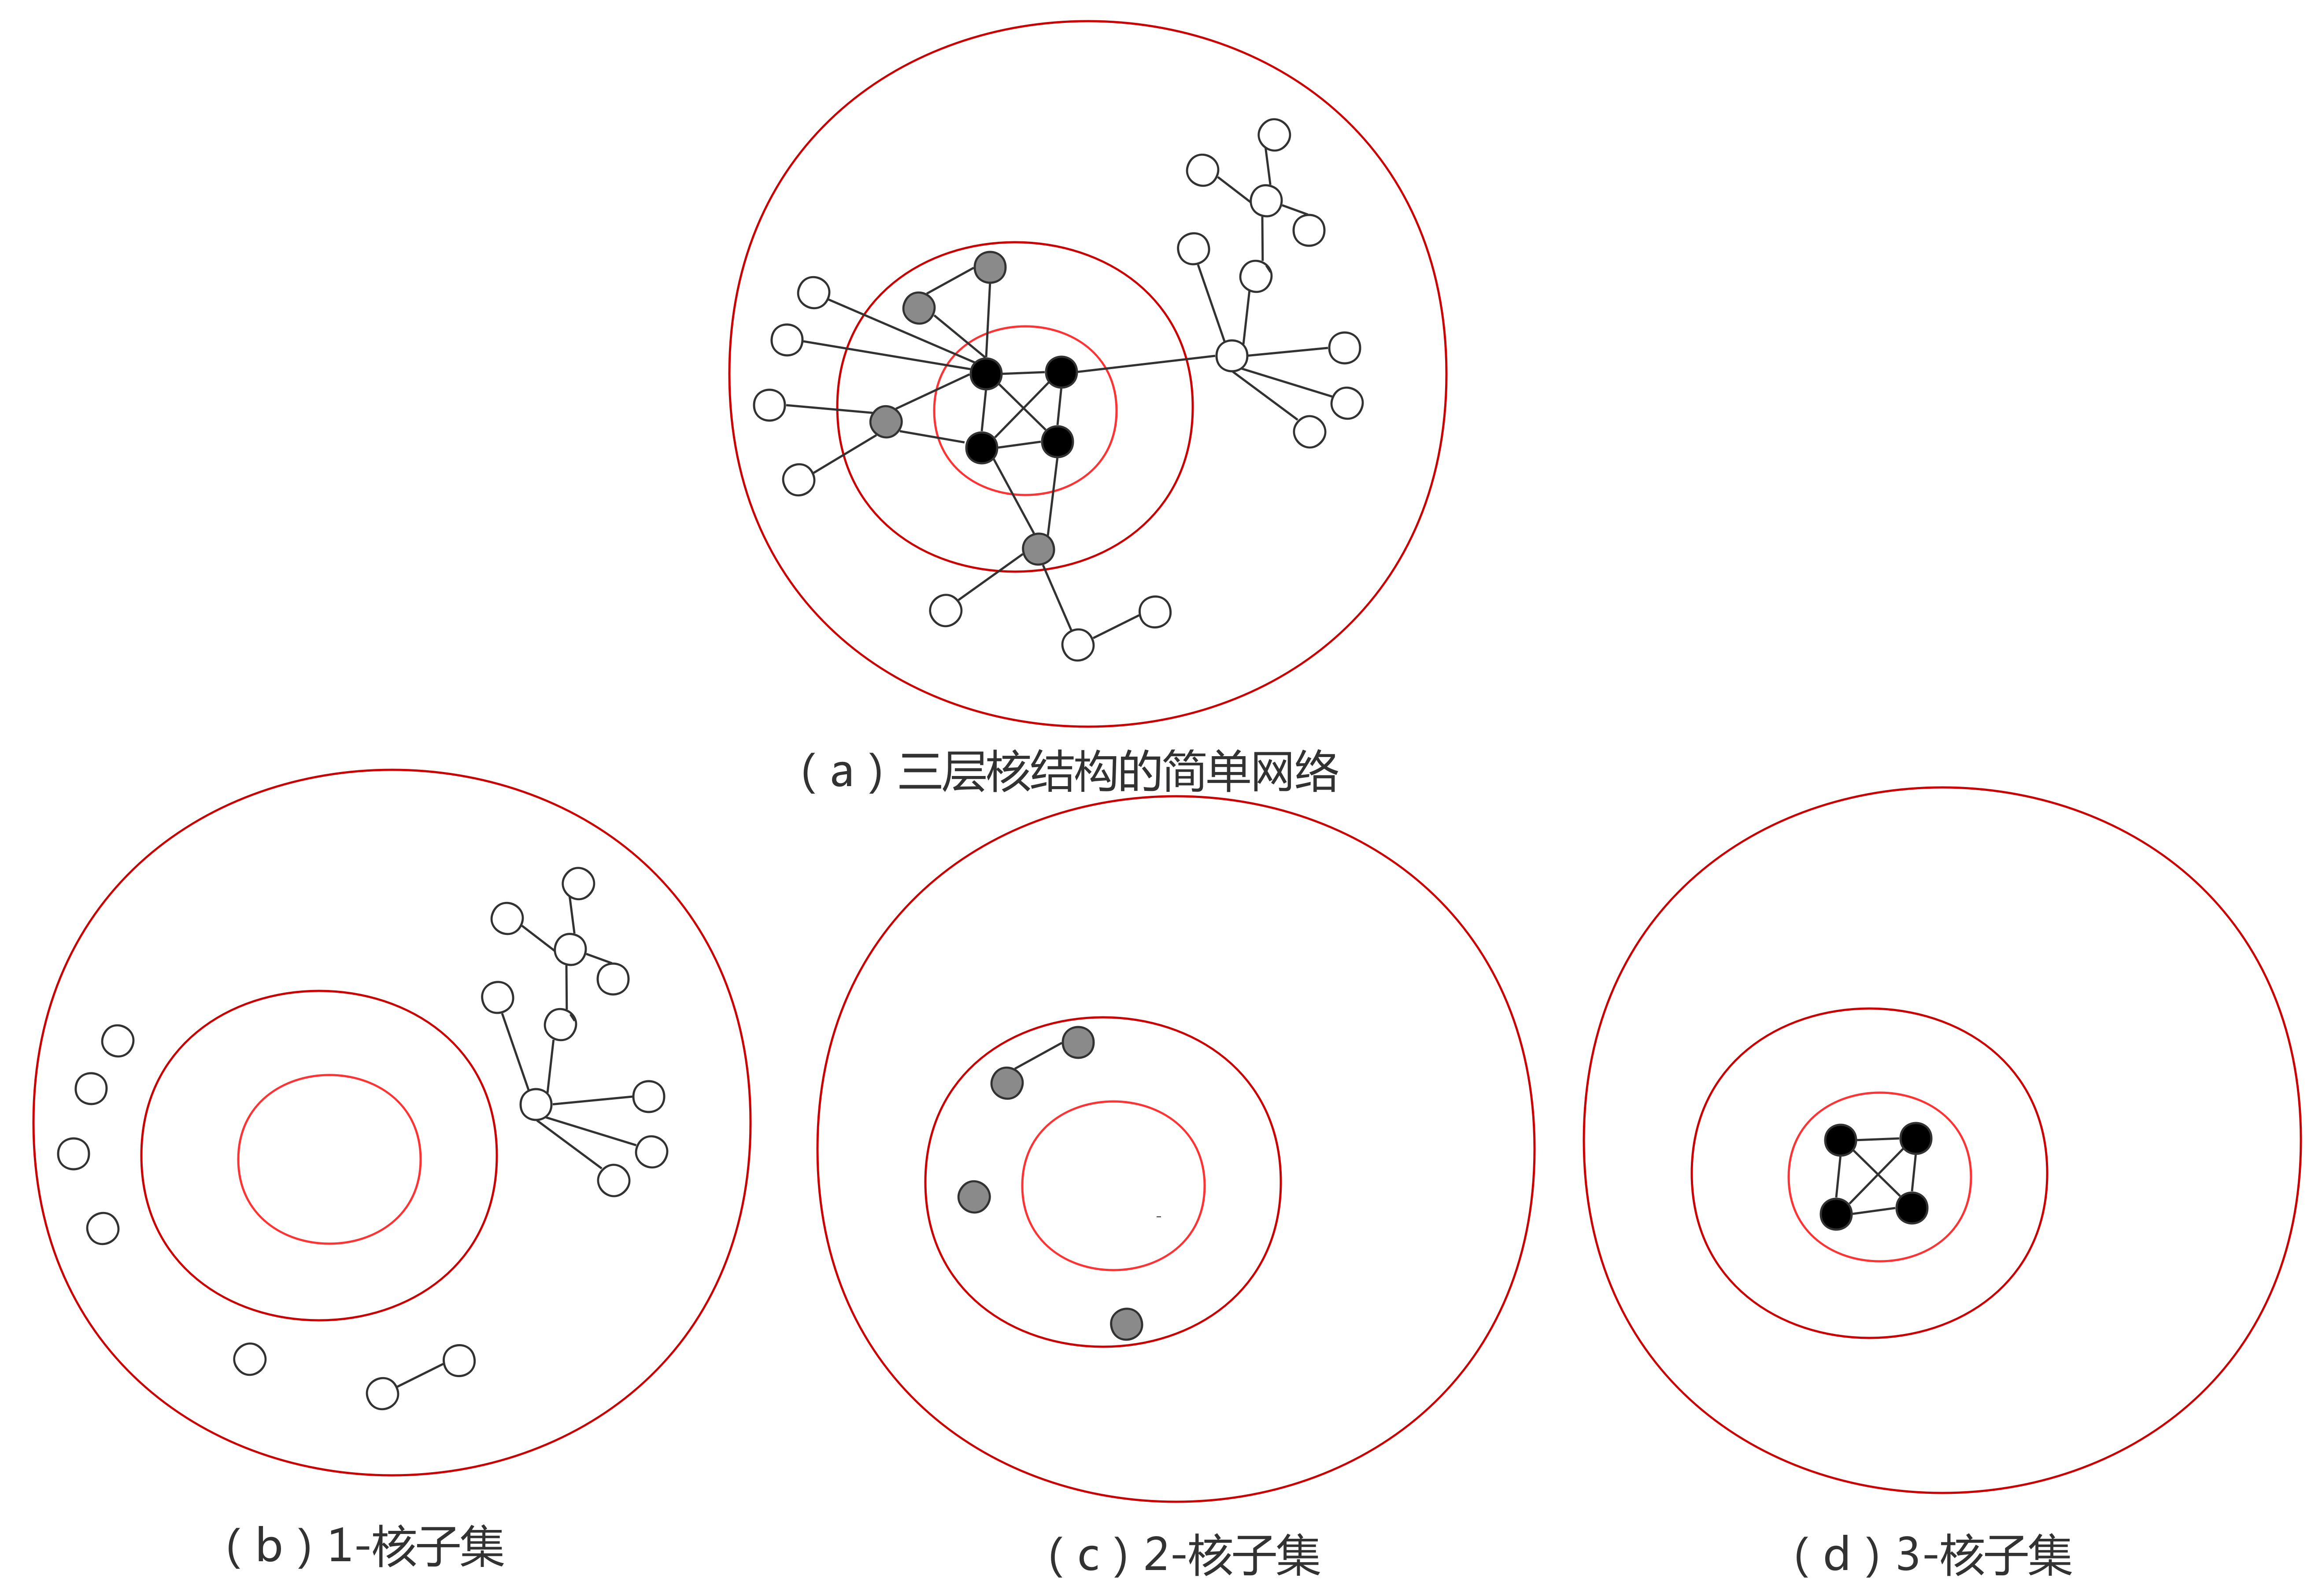
\includegraphics[width=0.75\textwidth]{figures/kcoreshili}
  \caption{k-核分解示意图}\label{fig:kcoreshili}
\end{figure}

节点的k-核值越大,表示它在网络中的位置越是中心,但是在复杂的社交网络之中,仍然存在大量具有相似k-核值的节点会随机的进行排序,因此仅仅依靠k-核值可能还无法较好的对节点进行排列。考虑到节点自身的影响力同样也受其邻居节点影响力的影响,某一节点若与其他关键节点均有连接,则可以认为此节点同样具有较大的影响力。

由此出发,本章提出了一种全新的节点影响力模型--NI(即Node Influence)。该模型在关注节点自身k-核值的同时,也考虑到了节点邻居的k-核值。节点i的影响力$NI(i)$的计算方式可参考公式\ref{eqn:NI}。

\begin{equation}
  \label{eqn:NI}
  NI(i)=Ks(i)+\alpha \cdot \sum_{j \in \Gamma _i} \frac{Ks(j)}{d_j}
\end{equation}

其中,$Ks(i)$上文已经提及,是节点i的k-核值;$\alpha$是用来调节邻居节点影响力的作用大小的可调参数,$\alpha \in [0,1]$;$\Gamma _i$表示的是节点i的邻居节点集合;$d_j$表示的是节点j的度。

按照节点影响力模型计算所有节点的NI值,把所有节点按照其NI值的大小降序排列,在每一轮标签迭代过程中就参照这一顺序进行节点标签更新,这样可以使得算法更加稳定,不再有随机性。

\subsection{标签选择方式上的改进}

在原始LPA算法中还有一大不稳定之处便是其标签选择方式,若一个节点更新标签的时候存在多个出现次数最多的邻居节点标签,原始LPA算法会随机选择其中一个。参考节点影响力模型的设计,本章提出算法在标签更新的时候也引进了节点影响力指标。

若节点i更新标签的时候,邻居节点中存在多个最多出现标签,则依次计算这些标签对节点i的影响力,最终选择影响力最大的标签进行更新;而在节点i更新标签,而邻居节点中存在唯一的最多出现标签的情况下,出于维持低时间复杂度的考虑,依然维持原始算法中的标签选择方式,直接更新节点标签为最多出现标签即可,不再进行无谓的标签影响力计算。此外,当发生极少可能的情况,即在进行了标签影响力计算之后,依旧无法确定采用哪个标签进行更新时,选择保留原标签,不进行任何更新。

公式\ref{eqn:LI}展示了标签$l$对节点i的影响力$LI(i,l)$的具体计算方式。

\begin{equation}
  \label{eqn:LI}
  LI(i,l)=\sum_{j \in \Gamma _i ^l} \frac{NI(j)}{d_j}
\end{equation}

在公式中,$\Gamma _i ^l$表示的是节点i的邻居节点中标签为$l$的节点集合。

% 此外,在标签选择方式上还值得一提的改进是:本章提出的算法在进行标签选择的时候,不仅仅会考虑邻居节点的标签,也会将自身的标签考虑在内。这同样也符合逻辑,以图\ref{fig:biaoqianbugenggai}为例进行分析,图中(a)为原始网络,对该网络进行标签传播时,显然所有节点均为1-核,而因为1号节点

% 而以公式\ref{eqn:LI}为基础的节点标签选择方式可参考公式\ref{eqn:ci}。
% \begin{equation}
%   \label{eqn:ci}
%   c_i=\arg\max_{l \in lmax} LI(i,l)
% \end{equation}

% 异步标签传播策略能够避免标签震荡现象,并且相对同步标签更新策略需要
% 更少的迭代次数,因此这里采用异步标签更新方法。然而由于节点并不是同时更
% 新的,因此节点更新的顺序对社区发现结果的稳定性及社区质量有很大的影响;
% 除此之外,标签传播过程中的标签选择策略也存在不稳定因素,当返回多个标签
% 同时被最大个数邻接点拥有时,LPA 算法随机的选择其中的一个标签作为该节点
% 的新标签,这也造成了 LPA 算法的不稳定性。而 下一章节要提到的COPRA 中也同样存在这些不稳
% 定因素。

% 在简单网络上分析传统标签传播算法的社区发现过程,如图\ref{fig:fig3-2}所示。在
% 该网络中有两个社区,分别是${v_1,v_2,v_3}$和${v_4,v_5,v_6}$。节点上的数字表示该节点
% 的社区标签,初始的时候各个节点的社区标签各不相同,如图\ref{fig:fig3-2}(a)所示。假设
% 经过几次标签传播之后,节点拥有相同的标签“2”,而节点 $v_4$、$v_5$和 $v_6$
% 的标签仍然各不相同,如图\ref{fig:fig3-2}(b)所示。如果首先更新节点 $v_4$
% 的标签,由于它的所有邻接点的标签都各不相同,随机选择标签“2”作为节点 $v_4$
% 的新标签,
% 更新结果如图\ref{fig:fig3-2}(c)所示;然后更新节点 $v_6$
% 的标签为标签“2”,此时节点 $v_5$
% 的两个邻接点的标签都为“2”,它也更新为标签“2”。这样更新后所有的节点都划分
% 到了同一个社区中,这样的社区划分结果没有意义。相反,在更新节点 $v_4$
% 的标签时,如果随机选择的更新标签是标签“6”,如图 \ref{fig:fig3-2}(d)所示;紧接着更新节点$v_5$
% 的标签,根据标签计算公式得到节点 $v_5$
% 的新标签为标签“6”;此时节点 $v_6$的
% 两个邻接点的标签都为“6”,它的标签保持不变。通过这样的标签更新顺序和标
% 签选择方式,能够得到正确的社区划分结果。
% \begin{figure}
%   \centering
%   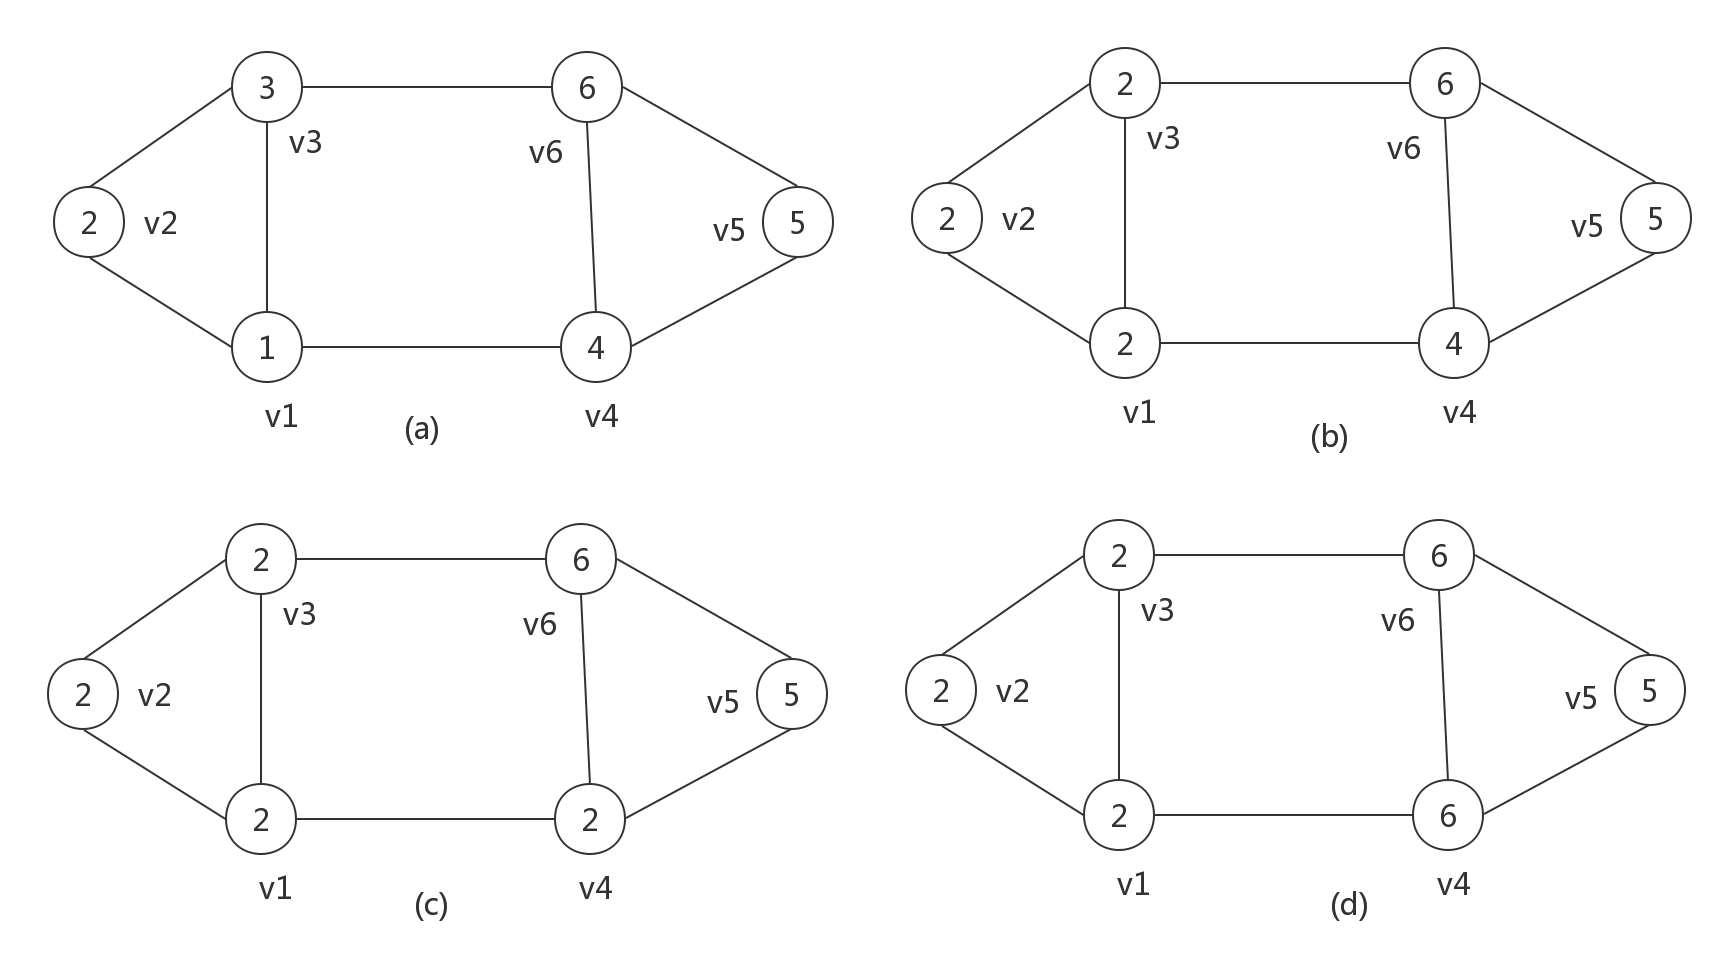
\includegraphics[width=0.75\textwidth]{figures/fig3-2}
%   \caption{标签传播过程示意图}\label{fig:fig3-2}
% \end{figure}

% \subsection{标签选择阶段的改进}
% 造成标签传播算法不稳定的另一个因素是标签选择的机制,当更新一个节点
% 的标签时,如果返回多个标签同时被最大个数的邻接点拥有时,传统的标签传播
% 算法会随机的从中选择一个标签赋给该节点,因此,算法迭代过程很难得到一个
% 稳定的收敛状态。为了提高算法的稳定性,当返回多个标签时,将节点影响值引
% 入到标签更新公式中,选择标签影响强度最大的标签赋给该节点。 

% 标签l对节点i的影响强度计算如公式\ref{eqn:LI}所示。
% \begin{equation}
%   \label{eqn:LI}
%   NI(i,l)=\sum_{j \in \Gamma _i} \frac{NI(j)}{d_j}
% \end{equation}
% 其中,$\Gamma _i$
% 表示节点i的邻接点中标签为l的节点集合。改进的节点标签更新公
% 式如公式\ref{eqn:ci}所示。
% \begin{equation}
%   \label{eqn:ci}
%   c_i=\arg\max_{l \in lmax} LI(i,l)
% \end{equation}
% 其中,$lmax $表示同时被最大个数邻接点拥有的标签集合。 
% 当传统标签传播算法的标签更新公式返回多个标签时,根据公式\ref{eqn:LI}计算这
% 些标签对该节点的影响强度,选择影响强度最大的标签赋给该节点。当标签影响
% 强度最大的标签仍有多个时,节点保留原有标签。 

\section{算法整体流程}

基于以上多项稳定性设计原则,本章提出的CDABSLP算法的在整体上主要可以分为初始化阶段、标签传播阶段两大部分。在标签传播阶段之后实际上还应有一个社区划分阶段,但是标签传播迭代完毕,网络中存在的每个标签即对应着一个社区,相应标签的节点即为属于该社区的节点,因此实质上,在标签传播结束就已经得到了相应的社区划分,后续唯一需要做的就是统计一下节点标签,将所有节点归类至相应社区,故本小节未将社区划分单独列为主要内容进行说明。图\ref{fig:cdabslp}为CDABSLP算法的整体流程图。

\begin{figure}
  \centering
  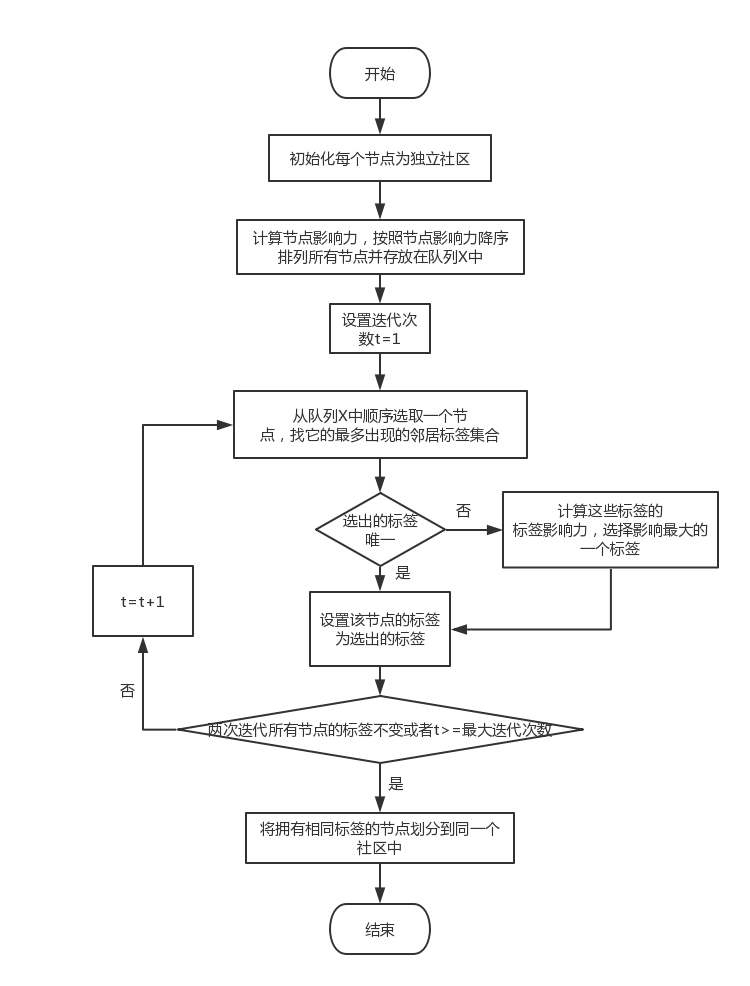
\includegraphics[width=1\textwidth]{figures/cdabslp}
  \caption{CDABSLP算法流程图}\label{fig:cdabslp}
 \end{figure}

下面结合一个实例来对CDABSLP算法的执行步骤进行详细说明,如图\ref{fig:CDABSLPshili}中所示。

\begin{figure}
  \centering
  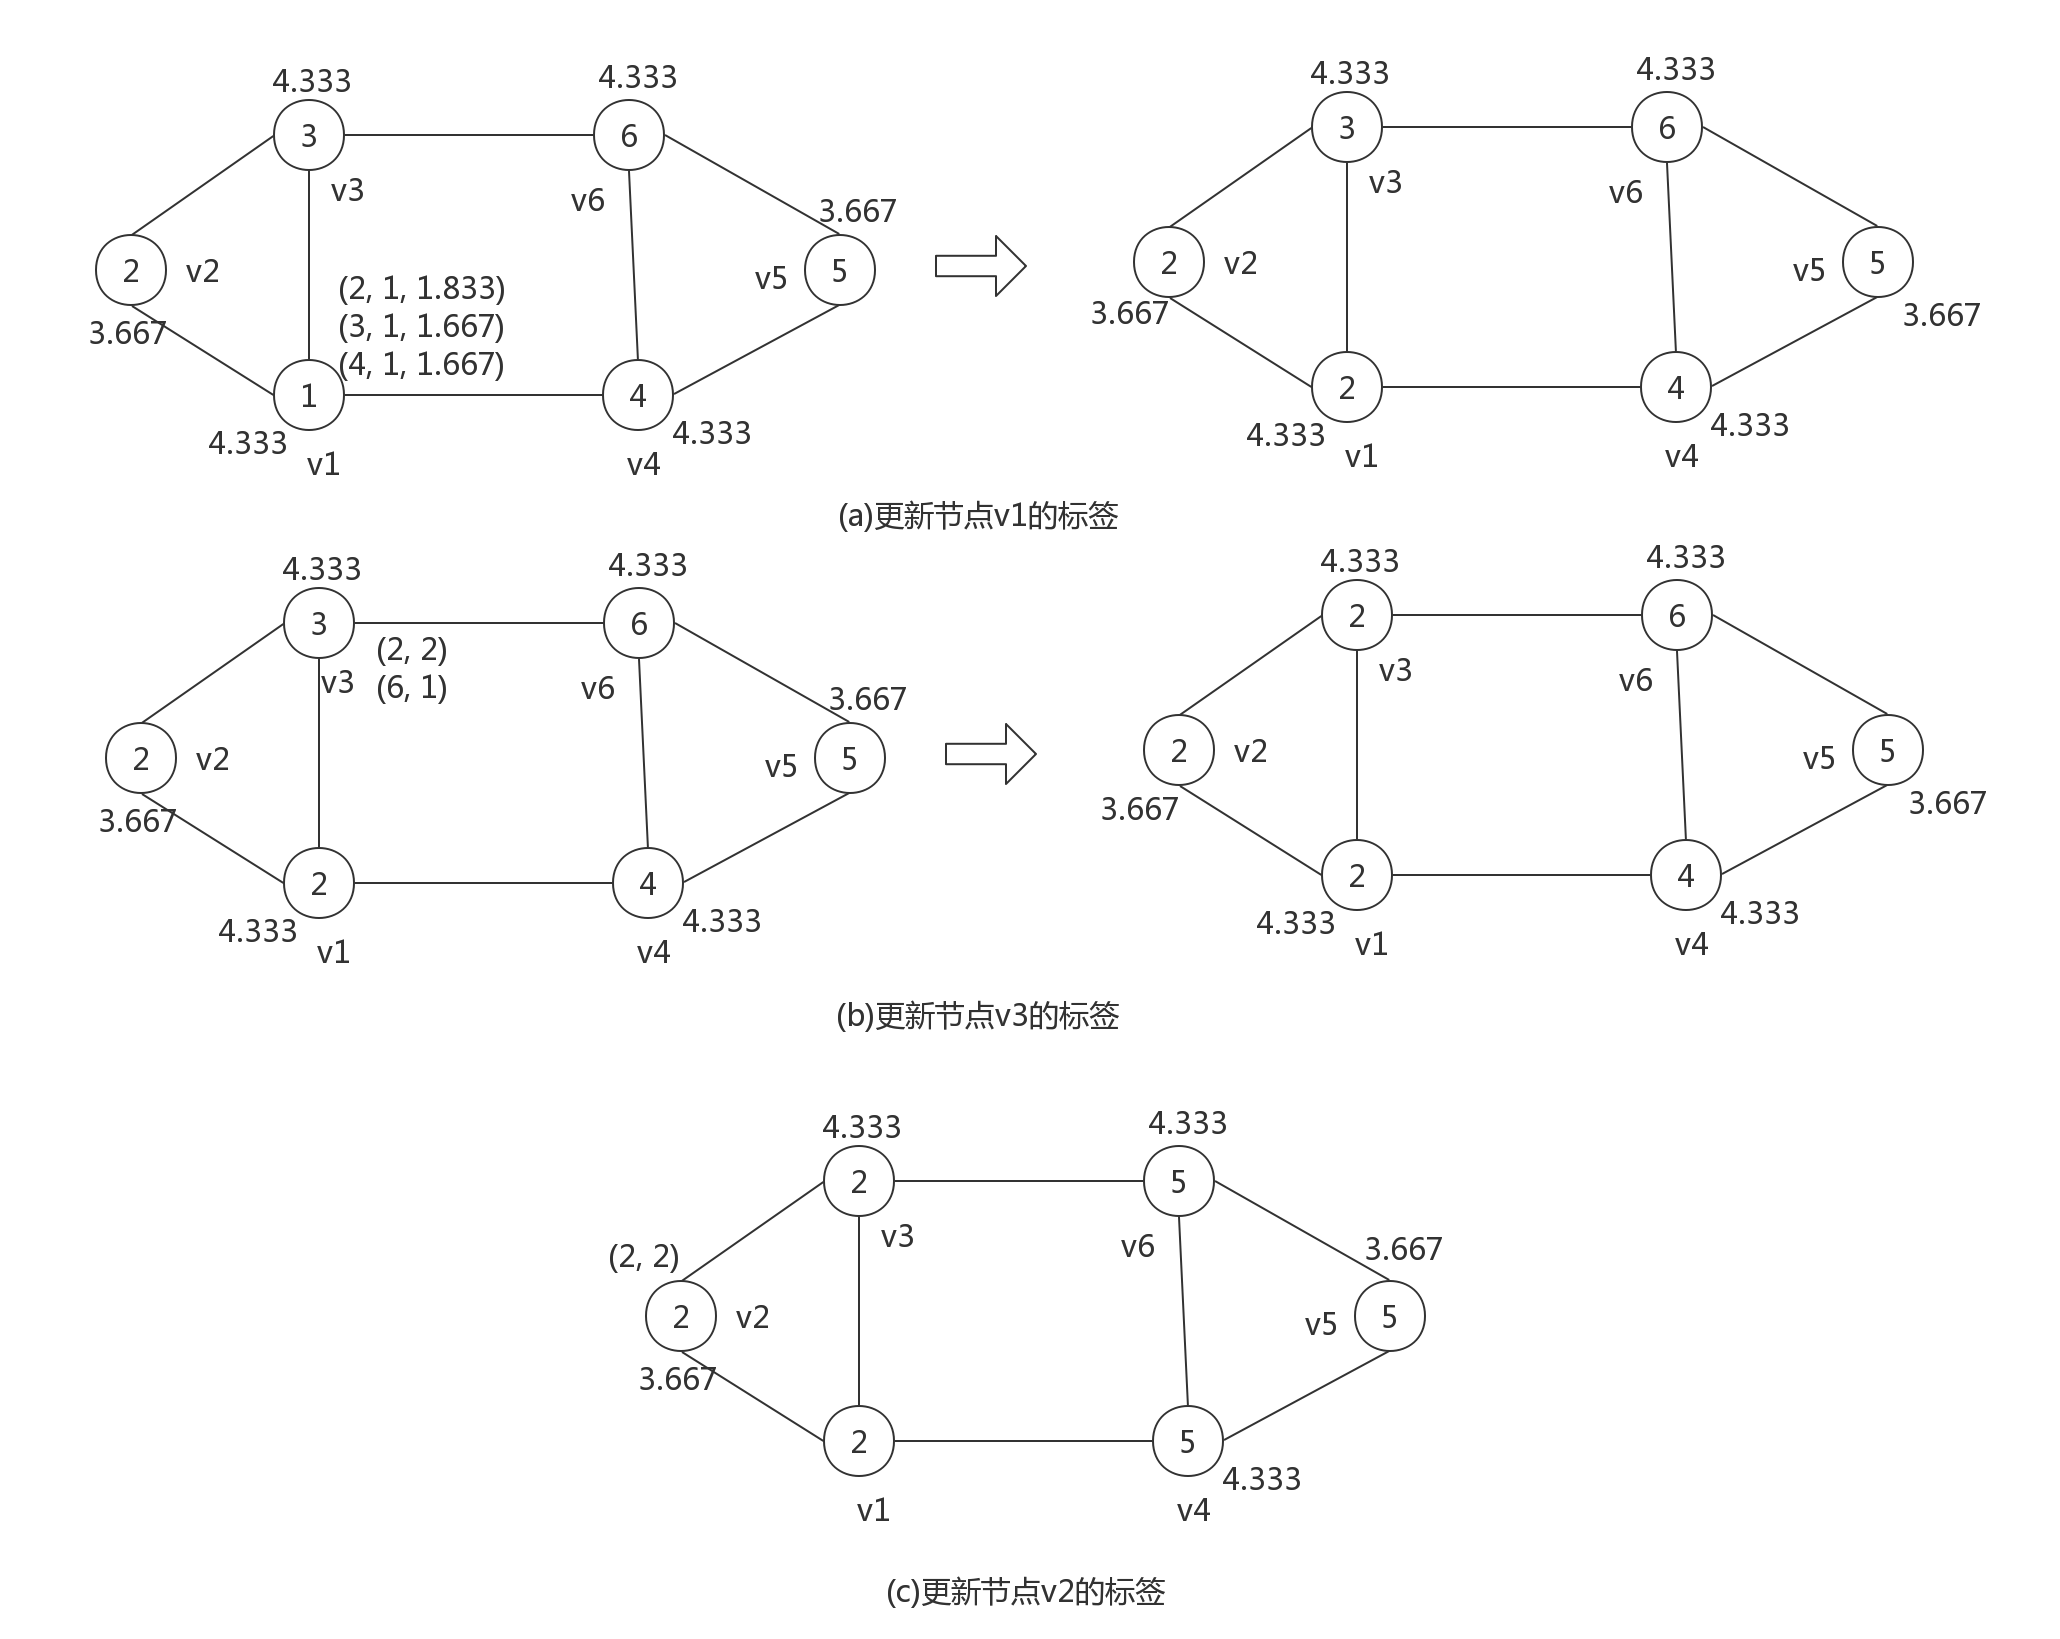
\includegraphics[width=0.75\textwidth]{figures/CDABSLPshili}
  \caption{CDABSLP算法标签传播过程示意图}\label{fig:CDABSLPshili}
 \end{figure}

\subsection{初始化阶段}

在算法的初始化阶段中:
\begin{enumerate}
  \item 每个节点被设置一个唯一的标签,即为其节点ID,在图\ref{fig:CDABSLPshili}中节点内的数字即为其初始化的标签,节点$\{ v_1,v_2,v_3,v_4,v_5,v_6 \} $的标签分别被初始化为$\{ 1,2,3,4,5,6 \} $;
  \item 对网络进行k-核分解,获取所有节点的k-核值$Ks(i)$,并在计算时,将中间过程中统计得出的每个节点的度保留下来以备下一步使用;
  \item 通过节点影响力公式\ref{eqn:NI}在初始化阶段计算每个节点的NI值,在图\ref{fig:CDABSLPshili}中每个节点外的浮点数值即代表其节点影响力大小,节点$\{ v_1,v_2,v_3,v_4,v_5,v_6 \} $的节点影响力分别为$\{ 4.333,3.667,4.333,4.333,3.667,4.333 \} $,此处小数点后仅保留了3位;
  \item 将所有节点以节点NI值大小降序排列,加入标签更新队列,NI值相同的节点,按照节点ID号升序排列,图\ref{fig:CDABSLPshili}所示的网络中,此排列即是按照$v_1-v_3-v_4-v_6-v_2-v_5$的顺序排列。
\end{enumerate}
CDABSLP算法初始化阶段具体可参考算法\ref{alg:CDABSLPchushihua}。

\begin{algorithm}[h]  
  \caption{CDABSLP算法初始化阶段}  
  \label{alg:CDABSLPchushihua} 
  \begin{algorithmic}[1]  
    \Require  
      社交网络$G=(V,E)$,节点影响力可调参数$\alpha$;  
    \Ensure  
      所有节点的影响力,标签更新队列;  
    \State 为网络G中每个节点设置一个唯一的标签,通常为其节点ID;  
    \State 对网络G进行k-核分解,获取所有节点的k-核值$Ks(i)$; 
    \State 通过节点影响力公式计算每个节点的节点影响力; 
    \State 将所有节点以节点影响力大小的降序进行排列后加入标签更新队列,节点影响力相同的节点,按照节点ID号升序排列; 
  \end{algorithmic}  
\end{algorithm}  

\subsection{标签传播阶段}

在算法的标签传播阶段中:
\begin{enumerate}
  \item 依次在标签更新队列中取出节点,找出它最多出现的邻居标签集合,在图\ref{fig:CDABSLPshili}(a)中展示了首先取出了节点$v_1$,它的三个邻居节点的标签各不相同,因此邻居标签最多出现次数为1,邻居标签集合即为$\{ 2,3,4 \} $;
  \item 判断找出的邻居标签集合是否唯一,若唯一则直接标签更新,若不唯一则按照公式\ref{eqn:LI}计算所有邻居标签的LI值,选择LI值最大的标签进行更新,若依然存在多个,则直接保留原标签,不进行更新,可以看见在图\ref{fig:CDABSLPshili}(a)中节点$v_1$的右上角有括号标注的三组数据,分别代表着标签$\{ 2,3,4 \} $分别出现了1次,对节点$v_1$的影响力分别为$\{ 1.833,1.667,1.667 \} $,此处小数点后仅保留了3位,显然标签“2”具有最大的影响力,故将节点$v_1$的标签更新为“2”,而在图\ref{fig:CDABSLPshili}(b)中可见CDABSLP算法在更新节点$v_3$的时候,因为标签“2”出现了两次,标签“6”仅出现一次,故将其更新为“2”,同理可按序将$\{ v_4,v_6,v_2,v_5 \} $更新为标签$\{ 5,5,2,5 \} $;
  \item 不断迭代直至标签不再更改或者已经达到最多迭代次数,在图\ref{fig:CDABSLPshili}中没有进行下一轮迭代的例图,但是不难知道,此例中的网络已经达到了最终收敛的稳定状态,结果也是符合预期的正确划分结果。仅仅只用了一轮标签传播,就在图\ref{fig:CDABSLPshili}所示网络中获得了稳定的划分状态,可见CDABSLP算法的输出结果是稳定而准确的。
\end{enumerate}
CDABSLP算法标签传播阶段具体可参考算法\ref{alg:CDABSLPlpa}。

\begin{algorithm}[h]  
  \caption{CDABSLP算法标签传播阶段}  
  \label{alg:CDABSLPlpa} 
  \begin{algorithmic}[1]  
    \Require  
      所有节点的影响力,标签更新队列,最大允许迭代轮数$maxIter$;  
    \Ensure  
      标签传播结果;  
    \State 迭代次数$iter=1$;  
    \Repeat  
      \State 在标签更新队列的队头取出节点$i$,找出它最多出现的邻居标签的集合$A = \{ l_1,l_2,...,l_m \} $;
      \If{$m==1$}  
        $//$找到的标签唯一
        \State 为节点$i$更新标签;  
      \Else  
        $//$找到的标签不唯一
        \State $max = 0$;
        \State $maxl = 0$;
        \For{each $l \in A$ }  
        $//$选择对节点$i$影响力最大的标签
          \State 计算$LI(i,l)$; 
          \If {$LI(i,l) > max$} 
            \State $max = LI(i,l)$;
            \State $maxl = l$;
          \EndIf 
          \State 将节点$i$标签更新为$maxl$;  
        \EndFor    
      \EndIf
      \State $iter = iter + 1$;  
    \Until{$iter > maxIter$ \textbf{or} 标签不再改变}
  \end{algorithmic}  
\end{algorithm}  

\section{算法时间复杂度分析}

CDABSLP算法的时间复杂度情况如下:

\begin{itemize}
  \item 所有节点初始化标签所花费的时间为$O(N)$;
  \item 所有节点影响力的计算所花费的时间为$O(M)$;
  \item 节点按照影响力大小降序排列所花费的时间为$O(N \cdot log(N))$;
  \item 标签迭代中的普通标签计算所花费的时间为$t \cdot O(M)$;
  \item 标签迭代中若遇到多个最大标签时,计算标签影响力所花费的时间为$t \cdot O(M)$;
  \item 社区划分过程所花费的时间为$O(N)$;
\end{itemize}

综上,CDABSLP算法的整体时间复杂度为:$2 \cdot O(N)+(2t+1) \cdot O(M)+O(N \cdot log(N))$;其中N,M,t分别表示节点总数、边的总数以及标签传播过程迭代次数,通常迭代次数不会很多,即相对于社交网络中N和M的大小,t一般仅是一个常数。可见CDABSLP算法在时间复杂度上虽然相较于原始LPA算法的线性复杂度有所增加,但是依然保持着很高的执行效率。

\section{验证实验}

本小节将为本章提出的CDABSLP算法进行实验验证。首先介绍实验的软硬件环境和采用的数据集,然后对算法的评价指标进行简单阐述,最后是相关对比实验的结果展示与分析,将CDABSLP算法与常用基准算法LPA算法和CNM算法\cite{Clauset2004Finding}进行对比,并与另一个基于LPA的改进算法KBLPA算法\cite{邓观明2016基于混合的}进行对比。考虑到LPA算法和KBLPA算法的实验结果不稳定,下面展示的实验结果均为多次实验的平均值。

\subsection{实验环境}

本章实现的CDABSLP算法所使用的机器配置如表\ref{tab:tab3-1}所示。CDABSLP算法使用Python语言编程实现,均基于Python的复杂网络相关软件包Networkx,使用Anaconda来对软件包进行管理和部署,具体配置如表\ref{tab:tab3-2}所示。

\begin{table}
  \centering
  \caption{计算机硬件配置} \label{tab:tab3-1}
  \begin{tabular*}{0.9\textwidth}{@{\extracolsep{\fill}}cccc}
  \toprule
    处理器			&2.2GHz 双核 Intel Core i7 \\
    内存容量			&8 GB 1600 MHz DDR3 \\
    硬盘容量			&128GB 固态硬盘 \\
  \bottomrule
  \end{tabular*}
% \end{table}

% \begin{table}
%   \centering
  \caption{计算机软件配置} \label{tab:tab3-2}
  \begin{tabular*}{0.9\textwidth}{@{\extracolsep{\fill}}cccc}
  \toprule
    操作系统			&macOS Sierra 10.12.6\\
    Anaconda版本  &conda 4.3.30 \\
    Networkx版本	&2.1 \\
    Python版本    &2.7.14\\
    Matplotlib版本  &2.0.2\\
    Numpy版本     &1.13.1\\
  \bottomrule
  \end{tabular*}
\end{table}

\subsection{数据集}

在本章的实验中,将分别采用真实网络中的数据集和LFR基准网络生成人工数据集来对CDABSLP算法的实验效果进行验证。
% 选用5个不同的真实数据集和LFR基准网络人工生成数据集进行实验验证本章所提算法的有效性。 

(1)真实数据集

在真实数据集中,本章实验选取了5个经典的数据集,包括Zachary Karate Club、American College Football、Dolphin Social Network等5个数据集。下面对这5个数据集进行简单介绍。

\begin{itemize}
  \item Zachary Karate Club数据集\cite{Zachary1977An}描绘的是美国一个大学空手道俱乐部34个成员彼此之间的社交网络,来自Zachary等人近3年的观察;因为其中主管和教练之间的矛盾,导致形成了两个小团体,即两个社区;在下文中将此数据集简记为N1。
  \item Dolphin Social Network数据集\cite{Lusseau2004Identifying}描绘的是新西兰一海湾居住的62只宽吻海豚彼此之间的社交网络,来自Lusseau等人长达7年的观察;在下文中将此数据集简记为N2。
  \item Pol Books数据集\cite{Polbooks}描绘的是根据在亚马逊上销售的政治相关书籍建立起来的政治派系网络,由Krebs等人通过人工分析而得,数据集中有自由派、中间派和保守派三个政治派系,即三个社区;在下文中将此数据集简记为N3。
  \item American College Football数据集\cite{football}描绘的是美国大学橄榄球比赛对阵情况,按照地区的不同,将各代表队分成了12个赛区,即12个社区;在下文中将此数据集简记为N4。
  \item Email数据集\cite{snapnets}描绘的是西班牙一大学里导师与研究生之间的邮件交互关系,由Guimer等人人工采集而得,该数据集并没有设定社区划分标准结果;在下文中将此数据集简记为N5。
\end{itemize}

真实数据集中的具体信息可参考表\ref{tab:tab3-3}。

% 在5个常用的真实网络数据集上进行实验验证本章算法的有效性,这5个真实网络数据集包括Karate、Dolphins 和 Football 等,各个数据集的详细信息如表\ref{tab:tab3-3}所示;

% N1:Karate是 Zachary 空手道俱乐部成员关系网络,网络中的所有节点对应各个成员,边表示两个端点对应的成员是好朋友。网络包含 34 个节点,78 条边和两个社区。 

% N2:Dolphins是 Lusseau 等人对栖息在新西兰 Doubtful Sound 峡湾的一个宽吻海豚群体进行长达 7 年的观察所构造出的海豚关系网,该群体包含 2 个家族共 62 只宽吻海豚。由这个群里的所有成员及它们间的接触关系构成一个包含62 个节点,159 条边和两个社区的网络。

% N3:Pol Books是从 Amazon 的图书销售记录抽象得到的网络数据集,分析了 105 本与美国政治相关的书和它们的 441 条共同销售关系,依据亚马逊上对图书的观点和评价情况,将这些书分为“自由派”、“中间派”和“保守派”三个类。因此,此数据集包含 105 个节点,441 条边和三个社区。

% N4:Football是分析美国高校橄榄球比赛对阵表得到的数据集。共有 115所高校派出代表队参赛,共进行了 616 场比赛,按各代表队地区的不同将这个包含 115 个节点 616 条边的网络分为 12 个社区。 

% N5:Email是由 Guimer 等人收集公布的,包含位于西班牙加泰罗尼亚自治区的罗维拉-威尔吉利大学(简称 URV)的教师和研究生之间的邮件往来关系。两个用户或者说两个邮箱地址如果互相发送过邮件,就构成一条边。网络包含 1133 个节点和 5451 条边。

\begin{table}
  \centering
  \caption{真实网络数据集} \label{tab:tab3-3}
  \begin{tabular*}{0.9\textwidth}{@{\extracolsep{\fill}}ccccc}
  \toprule
    数据集名称		&节点数   &边数   &社区数  &本文简称\\
  \midrule
    Zachary Karate Club  &34 &78 &2 &N1\\
    Dolphin Social Network	&62 &159  &2 &N2\\
    Pol Books  &105  &441  &3 &N3\\
    American College Football  &115  &616  &12 &N4\\
    Email     &1133 &5451 &- &N5\\
  \bottomrule
  \end{tabular*}
\end{table}

(2)LFR基准网络

在人工生成的基准网络之中,目前来说使用较为普遍的是GN基准网络\cite{2002Community}和LFR基准网络\cite{LFR}。早期的社区发现研究在进行实验分析时主要采用GN基准网络,但是无论如何调节设置参数z,GN基准网络生成的网络始终只有128个节点,这样的网络结构比较简单,因此也就缺少了很多真实社交网络中应有的特征。

而相对于GN基准网络,LFR基准网络深刻考虑到了真实社交网络中的“无标度”特征,可以自由对节点的度以及社区的大小等网络性质进行参数上的设置。因此,LFR基准网络已经成为当前最为流行的人工模拟数据集。在生成LFR人工数据集时需要设置的主要参数和它们的含义可参考表\ref{tab:tab3-4}。
% LFR基准网络是目前在社区发现领域使用最多的人工数据集之一。通过调整网络生成参数可以产生用户需要的不同的人工数据集,LFR 基准网络的主要生成参数及其含义如表\ref{tab:tab3-4}所示。

\begin{table}
  \centering
  \caption{LFR人工基准网络生成参数及其含义} \label{tab:tab3-4}
  \begin{tabular*}{0.9\textwidth}{@{\extracolsep{\fill}}cccc}
  \toprule
    参数		&含义\\
  \midrule
    N  &节点的个数\\
    avgk	&节点的平均度\\ 
    maxk  &节点的最大度\\
    minc  &最小社区包含的节点个数\\
    maxc  &最大社区包含的节点个数\\
    mu    &混合参数\\
    on    &重叠节点的个数\\
    om    &重叠节点最多可属于的社区个数\\
  \bottomrule
  \end{tabular*}
\end{table}

在表\ref{tab:tab3-4}中列出的所有参数里,需要进一步解释的是混合参数$mu$,$ mu \in [0,1]$。该参数表示的是社区内部节点与社区外部节点之间存在边的概率。在LFR人工数据集上进行社区发现的难度与$mu$参数值的大小成正比。$mu$越小,表明社区发现的难度越小,而$mu$越大,表明社区发现的难度越大。

为了能充分验证CDABSLP算法的效果,利用LFR基准网络生成程序生成了6组非重叠社区的人工数据集,将其编号分别记为$L1\sim L6$。具体参数设置可参考表\ref{tab:tab3-5}。其中所有生成网络中的maxk均设置为500,每组数据中按照mu参数从0.1到0.9分别生成9个数据集,而在非重叠社区数据集的生成过程中,on和om选择默认值0和1即可。
% 在 LFR 模型众多的生成参数中,混合参数$ mu \in [0,1]$是非常重要的一个参数,mu 越小,说明连接社区之间的边越少,社区之间越“分离”,社区划分的难度随着 mu 的增长而增大。on 和 om 两个参数用于生成具有重叠社区的数据集,生成具有非重叠社区结构的数据集时,只需将 on 设置为 0,om 设置为 1 即可。 
% 生成六组具有非重叠社区结构的 LFR 基准网络数据集,所有的网络共享的相同参数是 maxk = 500、on = 0 和 om = 1。每组包含九个 mu 值不同的数据集,分别为 0.1 到 0.9,每组中的九个数据集共享参数 N、avgk、minc 和 maxc。其他参数都取默认值。表\ref{tab:tab3-5}展示了这六组网络详细的生成参数情况。 

\begin{table}
  \centering
  \caption{LFR基准网络在非重叠社区数据集上的生成参数} \label{tab:tab3-5}
  \begin{tabular*}{0.9\textwidth}{@{\extracolsep{\fill}}ccccc}
  \toprule
    编号		&N  &avgk  &minc &maxc \\
  \midrule
    L1  &10000  &100  &10 &500 \\
    L2  &10000  &100  &20 &100 \\
    L3  &50000  &100  &10 &500 \\
    L4  &50000  &100  &20 &100 \\
    L5  &10000  &200  &10 &500 \\
    L6  &10000  &200  &20 &100 \\
  \bottomrule
  \end{tabular*}
\end{table}
% \begin{table}
%   \centering
%   \caption{LFR基准网络在非重叠社区数据集上的生成参数} \label{tab:tab3-5}
%   \begin{tabular*}{0.9\textwidth}{@{\extracolsep{\fill}}ccccccc}
%   \toprule
%     编号		&N  &avgk &maxk &minc &maxc &mu\\
%   \midrule
%     L1  &10000  &100 &500 &10 &500 &$0.1\sim 0.9$\\
%     L2  &10000  &100 &500 &20 &100 &$0.1\sim 0.9$\\
%     L3  &50000  &100 &500 &10 &500 &$0.1\sim 0.9$\\
%     L4  &50000  &100 &500 &20 &100 &$0.1\sim 0.9$\\
%     L5  &10000  &200 &500 &10 &500 &$0.1\sim 0.9$\\
%     L6  &10000  &200 &500 &20 &100 &$0.1\sim 0.9$\\
%   \bottomrule
%   \end{tabular*}
% \end{table}

\subsection{评价指标}

随着社区发现算法的不断提出,针对如何评判社区发现结果的优劣这一问题,研究人员们也同样提出了很多评价指标。本章将采用模块度、标准化互信息(NMI)和F-measure值。下面介绍这三个评价指标:
% 迄今为止,出现了各种各样的社区发现算法,如何评价不同的的发现算法的好坏是一个非常重要的问题。为此,学者们提出了多种社区结构评价指标用来评价网络社区划分质量,其中比较有代表性的有模块度、NMI等。下面介绍这些指标。

(1)模块度

模块度\cite{2002Community}是Newman等人在提出GN算法之后,用以解决当时的社区发现算法无法很好地衡量社区划分结果质量的问题,专门提出的用以评价社区划分结果的评价指标。模块度通过对比划分后的网络与随机网络在相同社区划分的情况下的社区内的连接密度来衡量社区划分的质量,其中的随机网络是与原始网络拥有同样节点度序列的随机网络。通常情况下将模块度即为Q,其具体计算方式可参考公式\ref{eqn:modular}。
% 模块度是目前学者们最常用和经典的网络社区结构评价指标,它最初是被Newman等人于2004年提出来的\cite{2002Community}。其通过比较现有网络和基准网络在相同社区划分下的连接密度差来衡量网络社区的优劣,其中基准网络是由原网络具有相同度序列的随机网络。模块度计算方式详见公式\ref{eqn:modular}。

\begin{equation}
  \label{eqn:modular}
  Q=\frac{1}{2m}\sum_{i,j}\left [ A_{ij}-\frac{k_ik_j}{2m} \right ]\delta (c_i, c_j)  
\end{equation}

其中,社交网络以邻接矩阵矩阵A表示,m代表着边的总数,$k_i$代表节点i的度数,$c_i$代表节点i被划分而得的社区编号。若$i=j$,则$\delta(c_i,c_j)=1$,反之$\delta(c_i,c_j)=0$
% 其中,A 表示网络中的邻接矩阵, m 表示网络中边的总数,$k_i$和$k_j$表示节点 i 和 j 的度数,表示节点 i 和 j 的度数,$c_i$和$c_j$表示节点 i 和 j 所属的社区。如果$i=j,\delta(c_i,c_j)=1$,反之$\delta(c_i,c_j)=0$

(2)标准化互信息(NMI)

模块度指标在对社区划分进行评判的时候,无需知道社区的标准划分结果,常用于没有标准划分的真实网络数据集之中,但是对于一些已经知道标准划分的数据集来说,文献\cite{Peng2014Weighting}中采用的标准化互信息(Normalized Mutual Information,一般缩写为NMI,中文翻译上也有学者将其译作“归一化互信息”)可以作为一个更为精确的衡量指标。NMI指数通常是被用于聚类之中,用于衡量两个聚类结果之间的相似程度,被引入社区发现领域后,已然成为了一个重要的社区划分结果优劣的衡量指标。它基本上能够较为客观地分析一个社区划分与标准划分相比而言的差距,能很好地评判划分的准确性。NMI指数的取值范围是0到1,数值越高表示社区发现结果越准确。它的计算方法可参考公式\ref{eqn:nmi}。
% 随着在线社交网络的发展,人们发现在线社交网络的很多数据中存在着暗示各个节点的社区属性信息。例如,在人人网的学校信息便揭示了网络节点中属于同一学校的社区结构,Facebook中的兴趣信息同样表征了具有相同兴趣的虚拟用户群体。这些数据在为社区发现问题提供了丰富的信息的同时,也在一定程度上为虚拟社区结构优劣的评判提供了标准答案。针对这种预先拥有一定虚拟社区结构信息的情况下,文献\cite{Peng2014Weighting}中提到了Normalized Mutual Information(NMI),利用信息化熵来衡量算法划分的社区结构和预先已知的社区结构之间的差异。NMI是基于混合矩阵(Confusion Matrix)N来计算的数字指标。NMI计算方式详见公式\ref{eqn:nmi}。

\begin{equation}
  \label{eqn:nmi}
  NMI=\frac{ -2 \sum_{i,j} N_{ij}  ln{\frac{N_{ij}}{N_iN_j}} } {\sum_{i}N_iln{\frac{N_i}{n}}+\sum_{j}N_jln{\frac{N_j}{n}}}
\end{equation}

其中,n代表网络中节点的总数,$N_i$表示社区i中的节点个数,$N_{ij}$代表的是社区i和社区j之间有连接的节点的总数。
% 使用该数字指标,可以衡量划分出来的社区结构与已知的网络社区结构的差异程度值,该值越大,则表明获得的社区结构划分越好,当该值达到最大化值1时,说明算法发现的社区结构与已知社区结构完全已知,效果最好。

\begin{figure}
 \centering
 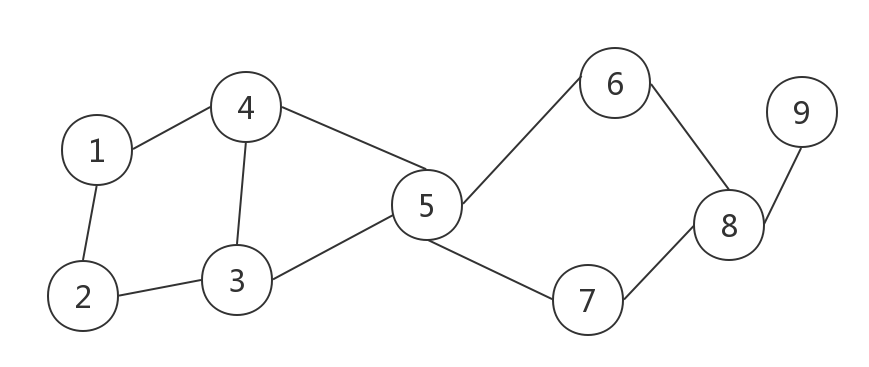
\includegraphics[width=0.75\textwidth]{figures/fig5-1}
 \caption{NMI网络示例图}\label{fig:fig5-1}
\end{figure}

% 下面以图\ref{fig:fig5-1}为例来说明计算NMI的过程。假设已知的最佳社区结构划分为集合{1,2,3,4}和{5,6,7,8},相应的社区划分向量表示为a = (1,1,1,1,2,3,3,3,3),再假设某算法获得的社区划分结构可以用向量表示为b = (3,3,3,3,2,1,1,1,1)来表示。根据已知的社区划分向量,可以构造混合矩阵\ref{eqn:n}。

% \begin{equation}
%   \label{eqn:n}
%   N=\begin{bmatrix}
%     0 & 0 &4 \\ 
%     0 & 1 & 0\\ 
%     4 & 0 & 0
%     \end{bmatrix}
% \end{equation}

% 根据上式计算可知,该划分的NMI值为1。

(3)PWF

成对F-measure值即Pairwise F-measure值,下文将采用缩写形式PWF来指导该指标。其计算方法具体可参考公式\ref{eqn:pwf}。
% 成对 F-measure(Pairwise F-measure,PWF)是成对准确率(Pairwise Precision,PWP)和成对召回率(Pairwise Recall,PWR)的调和,其计算如公式\ref{eqn:pwf}所示。

\begin{equation}
  \label{eqn:pwf}
  PWF=\frac{2\cdot PWP\cdot PWR}{PWP+PWR}
\end{equation}

其中PWP代表的是成对准确率(Pairwise Precision),PWP的计算公式具体可参考公式\ref{eqn:pwp};而PWR代表的是成对召回率(Pairwise Recall),PWR的计算公式具体可参考公式\ref{eqn:pwr}。
% 成对准确率(PWP)和成对召回率(PWR)的计算公式分别为公式\ref{eqn:pwp}和公式\ref{eqn:pwr}。

\begin{equation}
  \label{eqn:pwp}
  PWP=\frac{ \left | S \cap T \right |}{ \left | S \right |}
\end{equation}

\begin{equation}
  \label{eqn:pwr}
  PWR=\frac{ \left | S \cap T \right |}{ \left | T \right |}
\end{equation}

其中,T代表着在数据集的正确社区发现结果中属于相同社区的节点对集合,而S代表在经过社区发现算法之后网络的社区划分结果中属于相同社区的节点对集合,$S \cap T $ 即是两者的交集,表示划分正确的节点集合,而对集合S两端加绝对值$\left | S \right |$,表示集合S中的元素个数。

与NMI类似,PWF值的大小同样是与社区划分质量的优劣成正比。
% T 表示在真实的社区划分结果中,在同一个社区内的节点对集合;S 表示在测试算法得到的社区划分结果中在同一个社区内的节点对集合;$\left | S \cap T \right |$ 表示在真实的社区划分结果和测试划分结果中都在同一个社区内的节点对集合。PWF 的取值范围是 $0 \sim 1$,PWF 越大,说明社区划分的准确率越高。

\subsection{实验结果及分析}

(1)真实网络数据上的实验

本节首先对上文介绍的五个真实数据集进行对比实验,采用的评价指标为模块度和NMI。所有数据集最终得到的模块度Q值可参见表{tab:tab3-6},而由于数据集N5并没有标准网络划分结果,因此无法对其使用NMI评价指标,故$N1 \sim N4$数据集最终得到的NMI值可参见表\ref{tab:tab3-7}。考虑到LPA算法和KBLPA算法实验结果的不稳定性,为了更好地凸显其不稳定的结果,它们的模块度与NMI值将会以均值±最大偏差的形式来展示。
% 在数据集中介绍的5个真实网络数据集经常出现在社区发现的文献中,使用模块度 Q 和标准化互信息 NMI 作为前四个数据集上实验结果的评价指标,而另外一个数据集上仅使用模块度 Q 作为评价指标。表\ref{tab:tab3-6}和表\ref{tab:tab3-7}给出了四种对比算法在5个真实网络数据集上的实验结果,由于 N5 网络的真实社区结构未知,所以在表 3-8 中仅给出了前四个网络上实验结果的 NMI 值。每个数据集上得到的最优的 Q 和 NMI 值用粗体表示,LPA算法和 CDABSLP 算法得到结果的 Q 和 NMI 以平均值±最大偏差的形式表示。

\begin{table}
  \centering
  \caption{真实网络数据集实验的模块度大小对比} \label{tab:tab3-6}
  \begin{tabular*}{0.9\textwidth}{@{\extracolsep{\fill}}ccccc}
  \toprule
    编号		&LPA  &CNM &KBLPA &CDABSLP \\
  \midrule
    N1  &$0.286 \pm 0.28$  &0.355 &$0.083 \pm 0.22$ &0.433 \\
    N2  &$0.455 \pm 0.18$  &0.316 &$0.499 \pm 0.11$ &0.531 \\
    N3  &$0.479 \pm 0.14$  &0.275 &$0.459 \pm 0.08$ &0.507 \\
    N4  &$0.572 \pm 0.13$  &0.547 &$0.583 \pm 0.08$ &0.592 \\
    N5  &$0.370 \pm 0.26$  &0.425 &$0.293 \pm 0.23$ &0.437 \\
  \bottomrule
  \end{tabular*}
\end{table}

\begin{table}
  \centering
  \caption{真实网络数据集实验的NMI大小对比} \label{tab:tab3-7}
  \begin{tabular*}{0.9\textwidth}{@{\extracolsep{\fill}}ccccc}
  \toprule
    编号		&LPA  &CNM &KBLPA &CDABSLP \\
  \midrule
    N1  &$0.573 \pm 0.48$  &0.445 &$0.183 \pm 0.33$ &1 \\
    N2  &$0.516 \pm 0.29$  &0.436 &$0.491 \pm 0.24$ &0.662 \\
    N3  &$0.564 \pm 0.17$  &0.245 &$0.534 \pm 0.11$ &0.676 \\
    N4  &$0.853 \pm 0.14$  &0.646 &$0.659 \pm 0.12$ &0.898 \\
  \bottomrule
  \end{tabular*}
\end{table}

从表\ref{tab:tab3-6}中不难看出,四个算法中,CDABSLP算法划分得到的社区计算出的模块度是最大的,且结果相对稳定,这表明了算法在社区划分质量和算法稳定性上均取得了不错的效果。其中KBLPA算法在这几个数据集上的表现并未比LPA算法优化多少,尽管在稳定性上比LPA算法强了一些,但是依然存在着结果不稳定的问题,且整体划分质量反而有所下降;而CNM算法则介于LPA算法、KBLPA算法和CDABSLP算法之间,相对比较中庸,虽然划分质量一般,但是贵在稳定。

在表\ref{tab:tab3-7}中反应的NMI结果来看,CDABSLP算法的优势将显得更加明显。四个数据集上CDABSLP算法均取得了远大于CNM算法的NMI值,而在稳定性上,CDABSLP算法又远胜于另外两种基于标签传播的算法。

综上所述,CDABSLP算法在真实网络数据集上具有较好的稳定性,且发现结果质量良好。
% 从表\ref{tab:tab3-6}和表\ref{tab:tab3-7}可以看出,CDABSLP 算法得到社区结构的模块度 Q 比其他三种算法都高。同时,CDABSLP 算法在前四个网络上得到的社区结构的 NMI 值也是最优的。KBLPA 算法的稳定性优于 LPA 算法,但是 KBLPA 算法在几乎所有网络上得到社区结构的 Q 和 NMI都没有 LPA 算法好。实验结果表明,CDABSLP 算法能够得到比其他三种算法更好更稳定的社区检测结果。

(2)LFR人工基准网络上的实验

图\ref{fig:S1deNMIhePWF} $\sim$ \ref{fig:S6deNMIhePWF}分别展示的是上文数据集中所提到的利用LFR人工基准网络生成程序生成的6组数据集上的NMI值与PWF值的实验结果对比图。其中,左侧的折线图展示的是NMI值的对比结果,右侧的折线图展示的是PWF值的对比结果,两者的横轴均为混合参数mu。因为LPA算法和KBLPA算法的不稳定性,在折线图中表示这两者的曲线每个横坐标对应着三个值,分别是均值和上下最大偏差值。
% 图\ref{fig:S1deNMIhePWF} $\sim$ \ref{fig:S6deNMIhePWF}分别是四种算法在六组非重叠 LFR 基准网络数据集(S1$\sim$S6)上实验结果的 NMI 和 PWF 指标的对比图。横轴代表混合参数 mu,取值从 0.1 到 0.9;左侧六幅图的纵轴代表社区划分结果的 NMI 值,右侧六幅图的纵轴表示实验结果的 PWF 值。

\begin{figure}
  \centering
  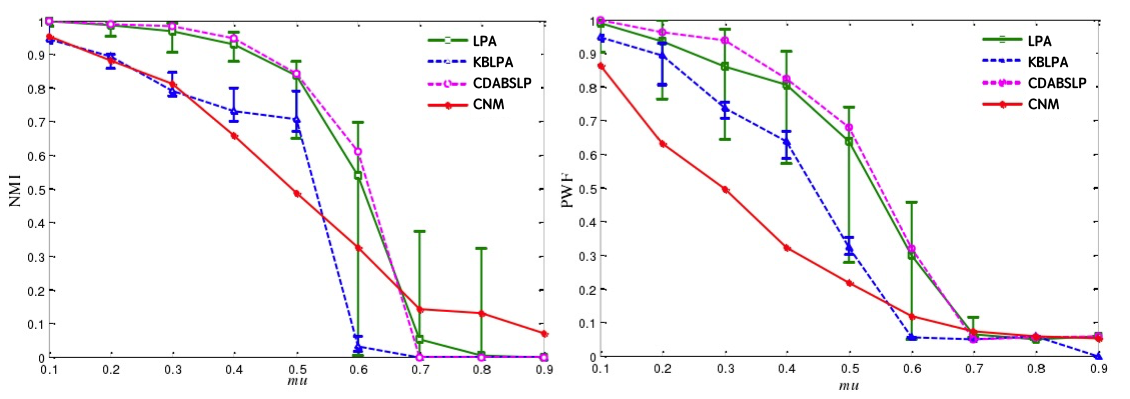
\includegraphics[width=0.75\textwidth]{figures/S1deNMIhePWF}
  \caption{L1网络上实验结果的NMI和PWF比较}\label{fig:S1deNMIhePWF}

  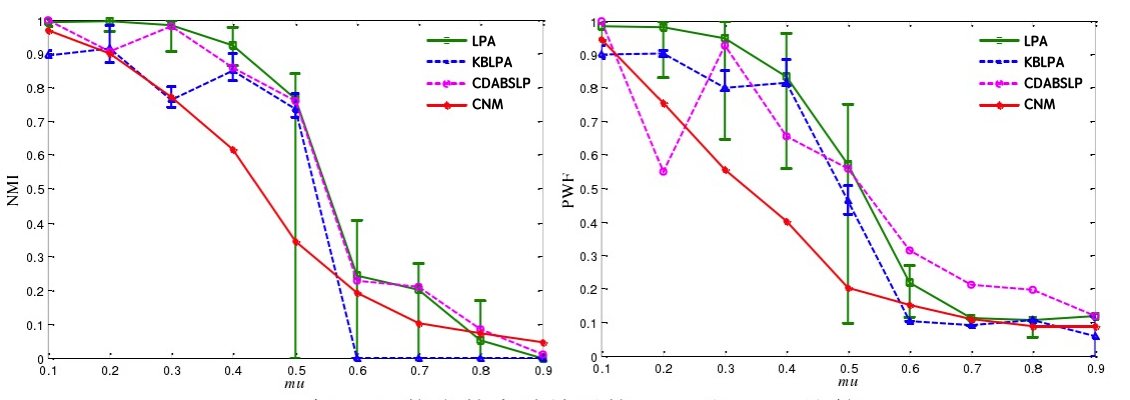
\includegraphics[width=0.75\textwidth]{figures/S2deNMIhePWF}
  \caption{L2网络上实验结果的NMI和PWF比较}\label{fig:S2deNMIhePWF}

  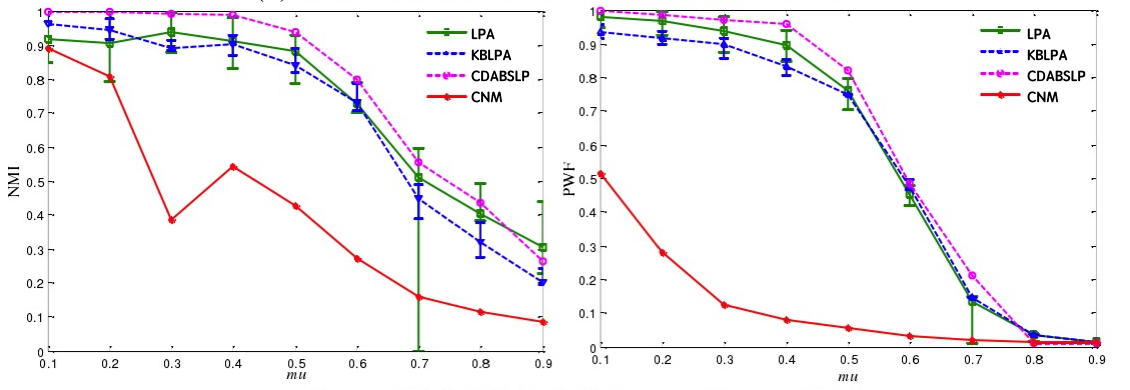
\includegraphics[width=0.75\textwidth]{figures/S3deNMIhePWF}
  \caption{L3网络上实验结果的NMI和PWF比较}\label{fig:S3deNMIhePWF}

  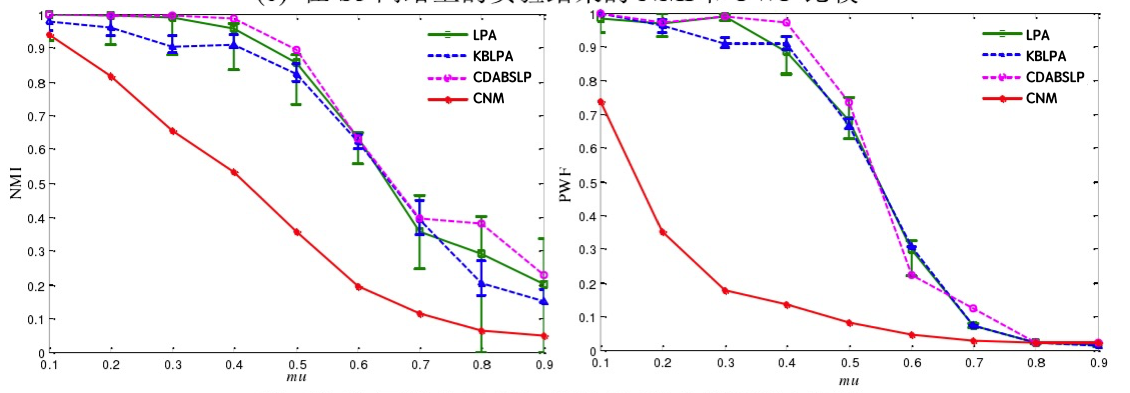
\includegraphics[width=0.75\textwidth]{figures/S4deNMIhePWF}
  \caption{L4网络上实验结果的NMI和PWF比较}\label{fig:S4deNMIhePWF}
\end{figure}

\begin{figure}
  \centering
  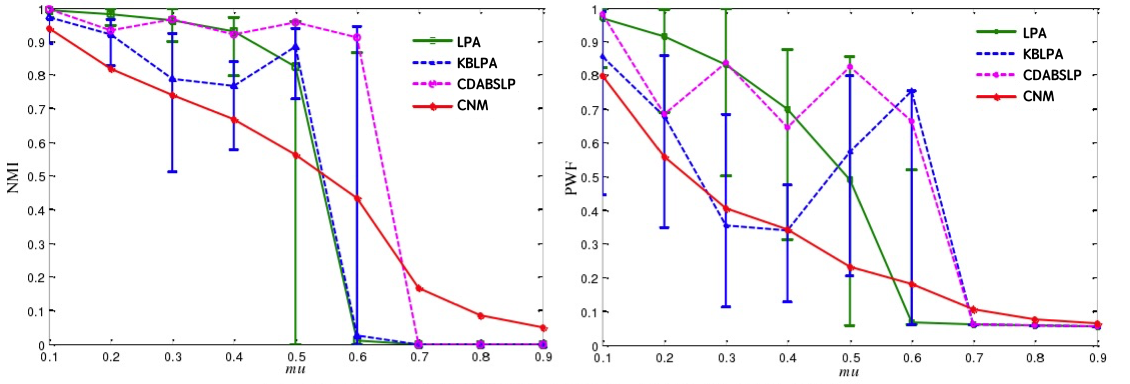
\includegraphics[width=0.75\textwidth]{figures/S5deNMIhePWF}
  \caption{L5网络上实验结果的NMI和PWF比较}\label{fig:S5deNMIhePWF}

  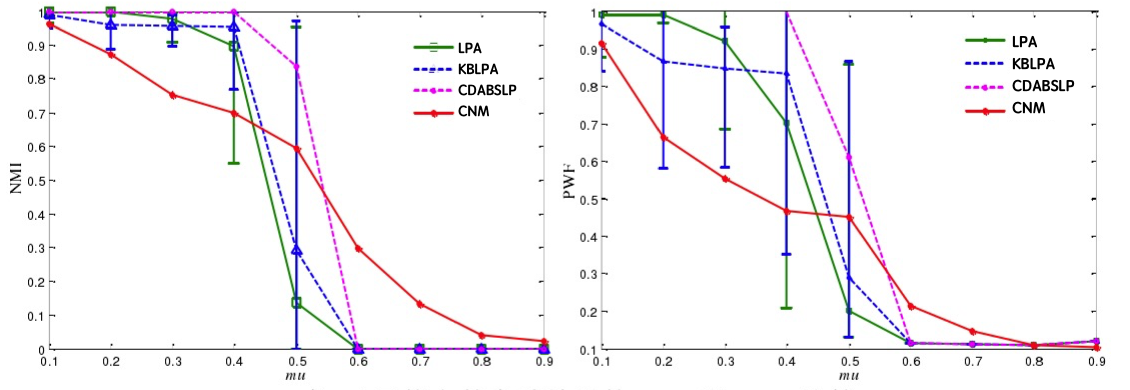
\includegraphics[width=0.75\textwidth]{figures/S6deNMIhePWF}
  \caption{L6网络上实验结果的NMI和PWF比较}\label{fig:S6deNMIhePWF}
\end{figure}

如\ref{fig:S1deNMIhePWF} $\sim$ \ref{fig:S6deNMIhePWF}中所示,所有的曲线都有一个逐渐下滑的趋势。当混合参数mu增大时,网络的社区划分结果开始变差,当混合参数大于0.5的时候,所有曲线都出现一个明显的下滑,这反映的其实是当网络的密度过高时,就很难再发现网络中的社区结构。当几乎所有的节点之间都有联系时,也就不存在了彼此之间联系孰轻孰重的考量。

虽然在这6组数据集上CDABSLP算法的表现也存在着一定的起伏的现象,例如在L1,L3,L4和L6数据集上有着较出色的结果,而在L2数据集上的实验结果并未超过LPA算法,但是整体而言,CDABSLP算法在混合参数mu较小的时候,图中CDABSLP的曲线都较为平滑,表明了CDABSLP算法良好的稳定性,且适应的网络密度范围也较广。在四个算法中,CNM算法对混合参数mu的依赖最大,随着mu的增大,CNM算法的曲线几乎呈正比下滑;而LPA算法虽然在某些次实验中能够取得不错的成绩,但是稳定性最差,上下偏差很大;KBLPA算法在稳定性上有了一定改善,但是依然不够稳定,且划分结果也不能令人满意。

综上所述,CDABSLP算法能够对具有良好社区结构的社交网络进行高质量的社区发现,且能保持良好的稳定性。
% 图\ref{fig:S1deNMIhePWF} $\sim$ \ref{fig:S6deNMIhePWF}中的 12 幅图可以看出,随着 mu 值的增大,网络的结构越来越复杂,社区结构越来越不明显,四种算法得到的社区划分结果都随之变差,尤其是当mu 大于 0.5 时,NMI 和 PWF 指标下降的更快。但是,整体来看,CDABSLP 算法的效果优于其他三种算法。虽然 CDABSLP 算法并不是在所有情况下都能得到最优的结果,但是它得到的结果是稳定的并且比较好的。从对比图中还能看出 LPA算法得到结果的 NMI 和 PWF 的波动都很大;KBLPA 算法得到的结果是比较稳定的,但是该算法检测得到的社区结构比 LPA 和 CDABSLP 算法都要差一些。在所有这些 LFR 网络上,CNM 算法并不能检测到最优的社区结构,而且它得到的社区的数目通常都比真实情况少。 

(3)可视化对比

本小节将通过可视化这一最为直观的手段来验证CDABSLP算法的社区发现结果的优劣。如图\ref{fig:Dolphins}所示的是Dolphin Social Network数据集的标准划分以及CDABSLP算法的社区发现结果。
% 将 CDABSLP 算法在 Dolphins 数据集上检测得到的社区结构和 Dolphins网络真实的社区结构进行比较,如图\ref{fig:Dolphins}所示。

\begin{figure}
  \centering
  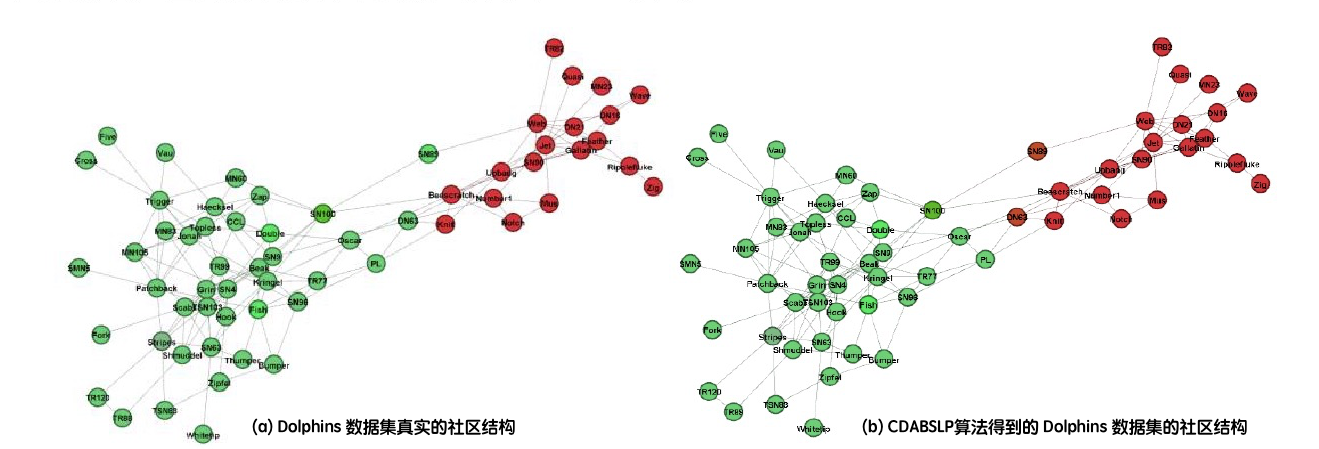
\includegraphics[width=0.75\textwidth]{figures/Dolphins}
  \caption{Dolphin Social Network数据集的社区结构}\label{fig:Dolphins}
\end{figure}

在图\ref{fig:Dolphins}中可见,节点以绿色和红色两种颜色标注以示区别,分别代表着两个社区。对比左侧的真实社区结构与右侧CDABSLP算法划分下的社区结构,除了两个节点的划分与真实社区结构中的不同外,容易看出两者几乎没有一模一样,这也就意味着CDABSLP算法几乎对该数据集进行了完全正确的划分。而值得一提的是,右侧图中的社区划分结果的模块度Q值是要大于左侧图中的模块度Q值的,考虑到Dolphin Social Network数据集的真实社区结构也是由研究人员根据多年观察人工进行的标注,所以也就是作为一个标准划分仅供参考而已。综上所述,可视化验证实验表明CDABSLP算法能够有效地发现社区结构。
% 图\ref{fig:Dolphins}(a)展示的是 Dolphins 网络真实的社区结构,节点不同的颜色表示不同社区;图\ref{fig:Dolphins}(b)是 CDABSLP 在 Dolphins 网络上检测到的社区结构图。通过比较这两幅图, CDABSLP 算法得到的结果中,节点 DN63 和 SN90 的划分与 Dolphins真实的社区结构不同。从 Dolphins 网络的拓扑结构发现,节点 DN63 有两个邻接点,它们分别属于两个不同的社区;节点 DN63 有五个邻接点, CDABSLP 算法将DN63 划分到了它的多数邻接点所在的社区。Dolphins 网络的真实的社区结构的模块度比 CDABSLP 算法得到的社区结构的模块度小,可以看出 CDABSLP 算法得到的结果是合理的。

(4)参数选择实验

在CDABSLP算法的节点影响力模型设计中,存在着一个调节参数$\alpha$,而为了考察该$\alpha$值的大小对算法性能的影响,本小节将针对不同的$\alpha$值进行实验。最终通过对不同大小$\alpha$值所对应的社区划分结果的NMI值的大小比较,判断该调节参数设置为何值时算法取最优解。
% 在 CDABSLP 算法中只有一个参数,即调节参数$\alpha$。为了分析参数对算法的影响,设置不同的参数$\alpha$值,在人工网络数据集上运行 CDABSLP 算法,通过比较结果的 NMI 分析参数对算法的影响。通过这种方法,能够发现参数$\alpha$取什么值时能够得到最好的结果。

利用LFR人工基准网络生成程序为此次实验生成5个人工数据集,除了平均节点度avgk取不同的值$ \{ 10,20,30,40,50 \} $外,其他参数取相同值,节点个数N设为1000,最大节点度设为50,社区包含最小节点数设为10,社区包含最大节点数设为50,混合参数mu设为0.1;而在实验过程中,$\alpha$分别从0取到1。图\ref{fig:alpha}为实验结果展示的折线图。
% 生成五个 LFR 基准数据集,参数 avgk 分别从 10 到 50,其他的生成参数相同(N = 1000、maxk = 50、minc = 10、maxc = 50 和 mu = 0.1)。图\ref{fig:alpha}显示了CDABSLP 算法在这些网络上的实验结果,横轴代表参数$\alpha$的不同取值,从 0 到 1,纵轴代表 NMI 值。

\begin{figure}
  \centering
  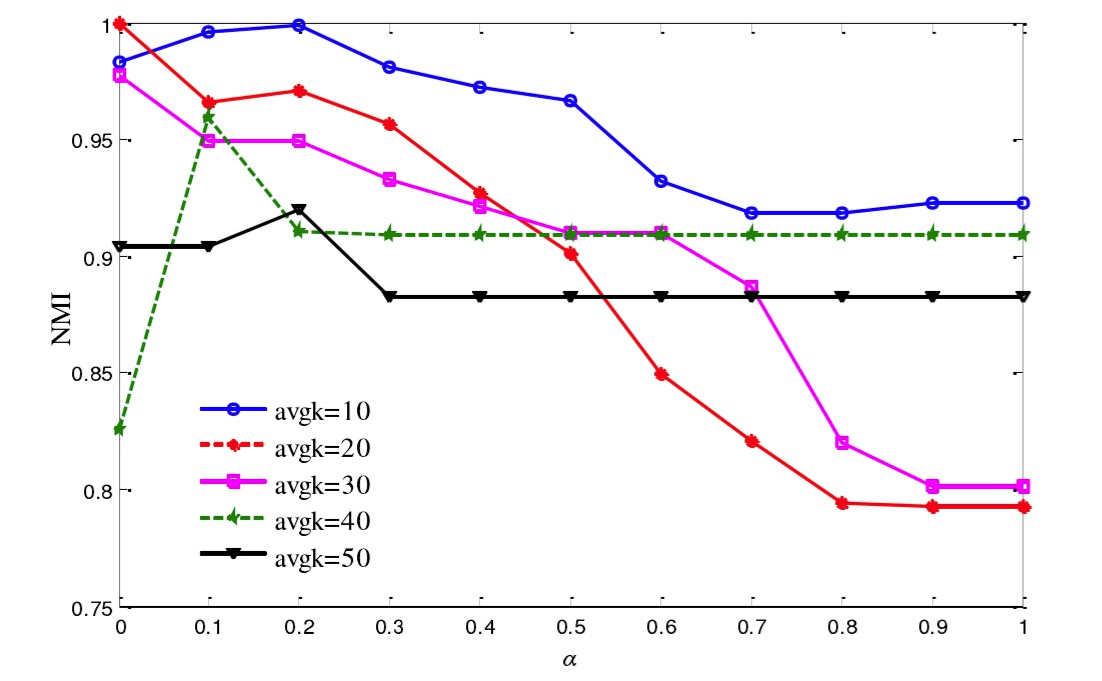
\includegraphics[width=0.75\textwidth]{figures/alpha}
  \caption{不同$\alpha$值对结果的影响}\label{fig:alpha}
\end{figure}

从图\ref{fig:alpha}中不难发现,每条曲线都有着各不相同的极大值,这表明了针对不同的网络密度,CDABSLP算法对应有不同的最优$\alpha$取值,因此也就无法简单的选择一个固定的$\alpha$值作为最优参数值。但是总体而言,可以认为0.2是一个相对而言较为合适的选择,可以将其设为调节参数$\alpha$的默认大小。此外,网络节点平均度avgk越大,参数$\alpha$大小对结果的影响就越小。
% 从图\ref{fig:alpha}中可以看出,参数$\alpha$取不同值的情况下,算法得到结果的 NMI 值变化很大。但是,对于每个网络,都存在一个最优的$\alpha$值使得 CDABSLP 算法能够得到 NMI 值最大的社区划分结果。此外,还能看出,在每个网络上得到的第一个极大值基本就是该网络上的最优值。

(5)不同规模网络的实验对比

生成十个不同规模的 LFR 基准网络数据集来验证算法的时间效率。网络中
节点个数设置为从 1000 到 10000 的十个不同的网络,其他的生成参数相同,均为
avgk = 10、maxk = 50、minc = 10、maxc = 50 和 mu = 0.1。 
图\ref{fig:butongguimowangluobijiao}左侧显示了四种算法在十个不同规模网络上运行时间的比较,图 \ref{fig:butongguimowangluobijiao}右侧
是左侧图的放大图,只显示了 LPA、KBLPA 和 CDABSLP 三种算法。

\begin{figure}
  \centering
  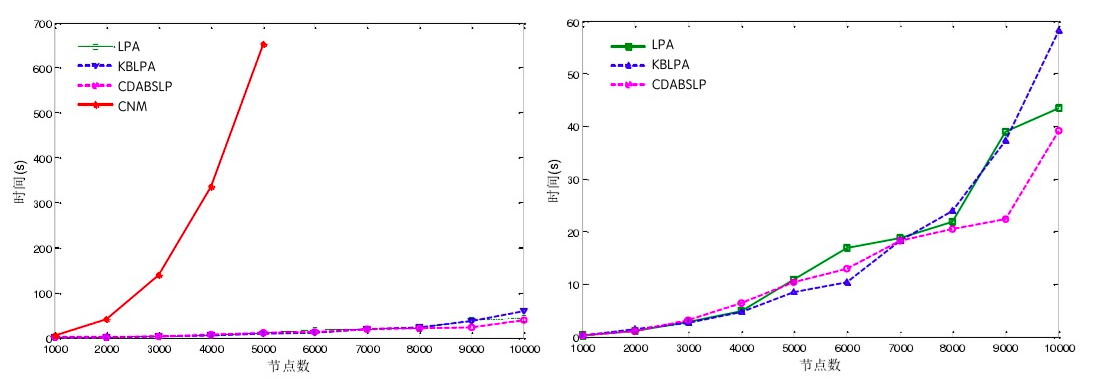
\includegraphics[width=0.75\textwidth]{figures/butongguimowangluobijiao}
  \caption{四种算法在不同规模网络上的效率比较}\label{fig:butongguimowangluobijiao}
\end{figure}

从图\ref{fig:butongguimowangluobijiao}可以看出,随着网络规模的增大,四种算法所用时间不断增加,其
中 CNM 算法所用时间是最长的,这是由于 CNM 算法迭代的次数远远多于其他
三种基于标签传播的算法的迭代次数。当网络规模大于 5000 时,由于计算机内
存限制 CNM 算法不能得到网络的社区结构。在图\ref{fig:butongguimowangluobijiao}右侧中,能更清楚的看到当
节点大于 7000 时,CDABSLP 算法所用时间比 LPA 算法少,说明 CDABSLP 算法比
LPA 算法更适合用于大规模复杂网络社区发现,这是因为 CDABSLP 算法的标签传
播迭代次数比 LPA 算法少,能够更快的趋于稳定。 


% \subsection{实验总结}

% CDABSLP算法从两个方面改善 LPA 算法不稳定的问题:首先,计算
% 网络中每个节点的节点影响值并按节点影响值降序排列作为节点标签更新的顺
% 序,取代传统 LPA 算法中节点更新顺序随机确定的方法;其次,在每次标签更
% 新迭代过程中,当传统的标签计算方法返回多个标签时,提出一种新的标签计算
% 公式,计算返回标签的影响强度,在返回的多个标签中重新选择一个影响强度最
% 大的标签作为该节点的新标签,以此替代传统 LPA 算法中随机选择一个标签的
% 方法。CDABSLP算法既保持了传统 LPA 算法的优点,还解决了 LPA 算法不稳定
% 的问题,该算法能够得到稳定的社区结构。大量实验结果表明CDABSLP算法的性
% 能优于目前一些代表性的社区发现算法。 

\section{本章小结}

本章主要介绍了一种基于稳定标签传播的非重叠社区发现算法,简称CDABSLP。在简单分析了原始LPA算法存在的缺陷之后,针对相应的缺陷逐一介绍其稳定性解决方案。算法在标签更新的时候采用异步更新的策略;然后提出了一种综合节点自身重要性以及邻居节点重要性的节点影响力模型,将节点更新顺序设为节点影响力的降序;最后在标签选择时出现多个最大标签的情况下,提出了一种标签影响力模型,在多个标签中,计算每个标签对当前节点的影响力,选取其中影响力最大的标签进行标签更新,当影响力最大的标签依然存在多个时,选择保留原标签不进行更改。通过真实网络以及人工网络中的验证实验,可知CDABSLP算法在具有良好的稳定性的同时兼具较高的运行效率,在多个评价指标之上社区发现准确率均有不错的表现。

%%==================================================
%% chapter04.tex for BIT Master Thesis
%% modified by 朱杰
%%==================================================
\chapter{基于稳定标签传播的重叠社区发现算法}

上一章中针对LPA算法的缺陷分析,本文提出了一种基于节点影响力模型的稳定的标签传播算法CDABSLP,然而该算法发现的是非重叠社区,本章将其核心思想引入基于LPA算法改进的重叠社区发现算法--COPRA算法\cite{Gregory2009Finding}之中,试图将其扩展至重叠社区发现领域。多标签传播算法(COPRA)在原始LPA算法的基础上,使得节点可以拥有不止一个标签,这样存在多个标签的节点即代表着隶属于多个社区。但是在保留了LPA算法执行速度快的优点同时,也继承了它不稳定的问题。
% 在验证了上一章所提稳定策略在 LPA 算法上的有效性的基础上,将此稳定策略运用到 COPRA 算法中,以验证其在重叠社区发现算法中的有效性。COPRA 算法\cite{Gregory2009Finding}和 SLPA 算法\cite{Xie2012SLPA}通过允许每个节点拥有多个标签的方法,将 LPA 算法扩展应用于重叠社区的发现,它们既继承了 LPA 算法的优点,也保留了 LPA 算法不稳定和鲁棒性差等缺点。COPRA 算法是最早的基于标签传播的重叠社区发现算法。

多标签传播算法是最早的基于标签传播思想的重叠社区发现算法,本章基于该算法以及上一章提出的CDABSLP算法在稳定性上的设计理念,将提出一种稳定的基于标签传播的重叠社区发现算法(Overlapping Community Detection Algorithm Based on Stable Label Propagation),下文简称OCDABSLP算法。

OCDABSLP算法采用了同步更新标签的策略,这点与CDABSLP算法不同;在标签选择方式上,对于邻居节点标签隶属度均小于既定阈值,且含有多个不同的最大隶属度标签的时候,选择最大隶属度标签中标签影响力模型计算值最大的那一个进行更新。在算法最终收敛之后,根据每个节点含有的标签将其划分到相应的社区,含有多个标签的节点即对应着存在于多个社区的重叠节点。
% 本章将会提出一种基于稳定标签传播的重叠社区发现算法(Overlapping Community Detection Algorithm Based on Stable Label Propagation),下文简称 OCDABSLP。OCDABSLP 算法在迭代执行标签更新过程中,当节点属于所有社区的隶属度都小于阈值且最大值有多个时,选择隶属度最大的多个标签中标签影响强度最大的标签。满足终止条件后,算法根据节点的标签将其划分到相应社区中,拥有多个标签的节点被划分到相应的多个社区中,成为重叠节点,得到最终的重叠社区划分结果。在不同复杂网络数据集上的大量实验表明本章算法能够得到比现有的大部分算法更好的社区划分结果。

%下面这段修改过了
本章接下来的内容组织结构上将先介绍一下多标签传播算法的情况,详细分析COPRA算法目前存在的缺陷;然后详细的阐述OCDABSLP算法在使得多标签传播更加稳定性上的设计;接着是对算法整体执行步骤进行全面的说明,并对算法时间复杂度进行分析; 最后在验证实验部分中,介绍了包括实验环境、实验数据集以及评价指标后,将会详细的分析在人工基准网络上的实验结果,通过与其他基准算法进行对比实验,以此来证明算法的效果。

\section{多标签传播算法的缺陷分析}

多标签传播算法(COPRA)\cite{Gregory2009Finding}最早是由Gregory 等人提出的第一个基于标签传播思想的重叠社区发现算法。COPRA算法是一种模糊性重叠社区发现算,它允许节点拥有不止一个标签,但是每个标签同时还需对应着一个隶属度,即代表着该节点隶属于该标签的模糊比例。在算法中每一个节点对应着一组$ \{ 标签,隶属度\} $对,通过不断的迭代获取所有节点最终的$ \{ 标签,隶属度\} $对,COPRA算法即可发现网络中重叠的社区结构。
% Gregory 等人\cite{Gregory2009Finding}提出的 COPRA 算法是第一个利用标签传播思想进行重叠社区发现的算法。算法中每个节点可以以不同隶属度拥有多个标签,每个节点包含一组标签-隶属度对$(l, b)$,$l $表示节点所属社区的编号,$b $表示节点属于该社区的隶属程度,$b_t(l, i)$表示在第$ t $次标签传播结束时节点$ i $属于社区$ l $的隶属程度。COPRA 通过迭代地更新各个节点的标签及隶属度来获取社区结构。

在初始化阶段,COPRA算法同样是为所有节点设置唯一的标签,同时把标签对应的隶属度初始化为1,表示此时每个节点都是自成一个社区,且仅属于自身标签代表的这一社区。接着在标签更新的过程中,采用同步更新,将节点的$ \{ 标签,隶属度\} $对更新为所有邻居节点中出现的标签和相同标签的平均隶属度对,同时删去其中隶属度小于既定阈值的标签,并将节点的标签隶属度重新归一化。若发生所有标签隶属度都小于既定阈值的情况,选择其中最大的进行保留;若最大隶属度的标签依然存在多个,则选择随机保留其中一个,然后进行归一化隶属度。在算法的社区划分阶段,按照节点拥有的标签将其划分至相应的社区即可。
% 与 LPA 算法相同,初始时,COPAR 算法为每个节点分配一个各不相同的标签,并将其隶属度设置为 1,即 $b_0(i, i) = 1$。然后采用同步更新策略进行标签更新迭代,在每次更新过程中,用邻接点中出现的所有相同标签的平均隶属度更新该节点的标签-隶属度对列表。每一轮更新后,删除隶属度小于 $\frac{1}{v}$ 的标签($v$ 是算法的参数),当一个节点的所有标签对应的隶属度都小于 $\frac{1}{v}$ 时,就只保留一个隶属度最大的标签,若此时有多个标签的隶属度同时取最大值,就随机保留隶属度最大的标签中的一个,然后对所有剩余标签的隶属度进行归一化。更新结束后,算法根据节点的标签将其划分到相应的社区中。一个节点最后拥有的标签数即为它被划分到的社区的个数。 

节点的标签隶属度计算方法可参考公式\ref{eqn:lishudu}。
% 函数 $b_t(l, i)$用于计算在第 $t $次迭代中,节点$ i $属于社区$ l $的隶属程度,计算如公式\ref{eqn:lishudu}所示。

\begin{equation}
  \label{eqn:lishudu}
  b_t(l,i)=\frac{\sum_{j\in \Gamma_i }b_{t-1}(l,j)}{d_i}
\end{equation}

其中,$d_i$代表节点i的度,$b_t(l,i)$的值即是节点i在第t轮迭代中隶属于标签l的程度。

多标签传播算法执行步骤的具体实现伪代码可参考算法\ref{alg:COPRA}。
% COPRA 算法的执行过程如算法\ref{alg:COPRA}所示。

\begin{algorithm}[htb]  
  \caption{多标签传播算法(COPRA)}  
  \label{alg:COPRA}  
  \begin{algorithmic}[1]  
    \Require  
      社交网络 $G = (V, E)$,最大迭代次数 $maxIter$,既定阈值$thr$;
    \Ensure  
      网络中所有的社区及其成员;  
    \State 初始化阶段:
    
    (a)标签-隶属度对的初始化:为所有节点设置初始标签,设为其节点ID即可,并将其隶属度设为1;

    (b)迭代次数初始化:迭代次数$iter = 0$;
    % 为网络中的每个节点分配一个各不相同的标签,标签-隶属度对集合为${(i,l)}$;
    
    %       令迭代次数$t=0$;  

    \State 标签传播阶段:

      (a)如果迭代次数$iter > maxIter$,停止标签传播,转步骤3;否则继续算法;
  
      (b)将网络中的节点按照随机顺序加入待更新标签队列;

      (c)针对队列中的每个节点,遍历其邻居节点,分别计算对于各邻居节点的标签的隶属度,将该节点的标签-隶属度对中的数据进行更新;

      (d)将更新后节点中标签隶属度小于既定阈值thr的标签删除;

      (e)对节点的所有标签-隶属度对进行归一化处理;

      (f)每轮标签传播迭代完毕,对比上一轮迭代结果,若标签集合不再发生变化,则停止标签传播,转步骤3;反之令$(iter = iter+ 1)$,转步骤2,继续下一轮迭代;
    % (a)如果迭代次数 $t > maxIter$,标签传播迭代过程结束,转 Step3;否则继续算法。 

    % (b)对于每个节点$v_i\in V$,根据公式\ref{eqn:lishudu}计算该节点属于其邻接点集合中出现的所有标签的隶属度,更新标签-隶属度对列表。根据参数$v$删除不满足条件的标签,并对剩余标签进行归一化。 
     
    % (c)如果连续两次迭代结束后,标签集合的大小不变,那么标签传播迭代过程停止,转Step3;否则,令$t = t+1$转到步骤(a)继续执行。

    \State 社区划分阶段:将具有相同标签的节点划分为一个社区,整个网络中存在的标签数量即是发现的社区数量,含有多个标签的节点即为重叠节点。
  \end{algorithmic}  
\end{algorithm} 

多标签传播算法在保留了原始LPA算法执行速度快的优点同时,也继承了它不稳定的问题,且容易把所有项点分配给一个社区,有些时候还可能会划分出一些无意义的社区。
% COPRA 算法继承了 LPA 算法的优点,也保留了 LPA 算法稳定性和鲁棒性差等缺点,且容易把所有项点分配给一个社区,有些时候还可能会划分出一些无意义的社区。

\section{算法核心思想}

\subsection{同步更新标签}

在CDABSLP算法中使用的是异步更新标签,为的是防止标签传播过程中产生震荡,且加快收敛速度,但是那是在非重叠社区发现中的有效手段,而在重叠社区发现算法中,由于节点本身就具有多标签,因此不会出现LPA算法中才会遇到的标签震荡问题。如若使用异步更新标签,在多标签传播过程中,甚至反而会导致标签混乱,致使最终结果出现失真现象,不具有复现性。

综上所述,在本章提出的OCDABSLP算法中,将会延续使用同步更新标签的策略。

\subsection{标签选择阶段的改进}

COPRA算法中存在的最大不稳定因素即是当发生所有标签隶属度都小于既定阈值的情况,且恰好最大隶属度的标签依然存在多个的时候,会选择随机保留其中一个。针对该随机性进行稳定性改进,不再进行随机选择,而是引入上一章节中提出的标签影响力模型,在重叠社区发现上对其进行扩展,设计了在多标签传播中的标签影响力模型NI,由原来的随机选择,改进为选择NI值大的标签,其计算方式可参考公式\ref{eqn:LI2}。
% 原始COPRA算法中的唯一一个不稳定因素是当节点属于所有社区的隶属度都小于阈值且最大值有多个时,会随机选择一个标签。因此,在此处对 COPRA算法进行改进。当出现上述情形时,选择隶属度最大的多个标签中标签影响力最大的标签。当标签影响力最大的标签仍有多个时,保留所有标签影响强度最大的标签。标签影响强度的计算如公式\ref{eqn:LI2}所示。

\begin{equation}
  \label{eqn:LI2}
  NI(i,l)=\sum_{j \in \Gamma _i} b_{t-1}(l,j) \frac{NI(j)}{d_j}
\end{equation}

\section{算法整体流程}

基于以上两项稳定性设计原则,本章提出的OCDABSLP算法的在整体上主要可以分为初始化阶段、标签传播阶段两大部分。在标签传播阶段之后实际上还应有一个社区划分阶段,但是标签传播迭代完毕,网络中存在的每个标签即对应着一个社区,相应标签的节点即为属于该社区的节点,因此实质上,在标签传播结束就已经得到了相应的社区划分,后续唯一需要做的就是统计一下节点标签,将所有节点归类至相应社区,故本小节未将社区划分单独列为主要内容进行说明。图\ref{fig:ocdabslp}为 OCDABSLP 的算法流程图。

\begin{figure}
  \centering
  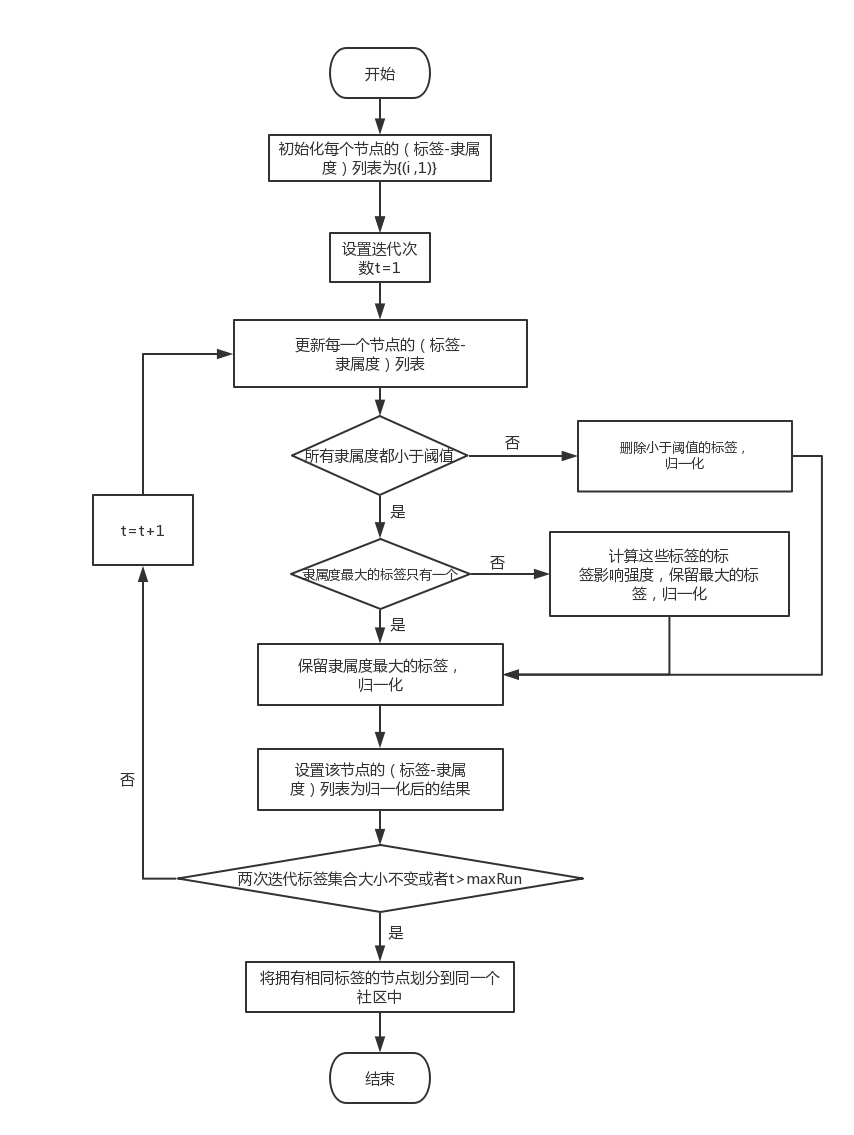
\includegraphics[width=1\textwidth]{figures/ocdabslp}
  \caption{OCDABSLP算法流程图}\label{fig:ocdabslp}
\end{figure}

\subsection{初始化阶段}

在算法的初始化阶段中:
\begin{enumerate}
  \item 初始化每个节点的(标签-隶属度)列表为$ \{ (i,1) \} $;
  \item 对网络进行k-核分解,获取所有节点的k-核值$Ks(i)$,并在计算时,将中间过程中统计得出的每个节点的度保留下来以备下一步使用;
  \item 通过节点影响力公式\ref{eqn:NI}在初始化阶段计算每个节点的节点影响力,以备后续计算标签影响力大小使用;
  \item 将所有节点以节点NI值大小降序排列,加入标签更新队列,NI值相同的节点,按照节点ID号升序排列。
\end{enumerate}
CDABSLP算法初始化阶段具体可参考算法\ref{alg:OCDABSLPchushihua}。

\begin{algorithm}[h]  
  \caption{OCDABSLP算法初始化阶段}  
  \label{alg:OCDABSLPchushihua} 
  \begin{algorithmic}[1]  
    \Require  
      社交网络$G=(V,E)$,节点影响力可调参数$\alpha$,标签隶属度阈值参数$v$;  
    \Ensure  
      所有节点的影响力,标签更新队列;  
    \State 初始化每个节点的(标签-隶属度)列表为$ \{ (i,1) \} $;  
    \State 对网络G进行k-核分解,获取所有节点的k-核值$Ks(i)$; 
    \State 通过节点影响力公式计算每个节点的节点影响力; 
    \State 将所有节点以节点NI值大小降序排列,加入标签更新队列,NI值相同的节点,按照节点ID号升序排列; 
  \end{algorithmic}  
\end{algorithm}  

\subsection{标签传播阶段}

在算法的标签传播阶段中:
\begin{enumerate}
  \item 更新每一个节点的(标签-隶属度)列表;
  \item 若隶属度不都小于阈值,删除小于阈值的标签,并进行归一化;
  \item 若隶属度都小于阈值且隶属度最大的标签唯一,是则保留隶属度最大的标签,并进行归一化;
  \item 若隶属度都小于阈值且隶属度最大的标签不唯一,计算这些标签的标签影响强度,保留最大的标签,并进行归一化;
  \item 设置该节点的(标签-隶属度)列表为归一化后的结果;
  \item 不断迭代直至标签不再更改或者已经达到最多迭代次数。
\end{enumerate}
CDABSLP算法标签传播阶段具体可参考算法\ref{alg:OCDABSLPlpa}。

\begin{algorithm}[h]  
  \caption{OCDABSLP算法标签传播阶段}  
  \label{alg:OCDABSLPlpa} 
  \begin{algorithmic}[1]  
    \Require  
      所有节点的影响力,标签更新队列,最大允许迭代轮数$maxIter$;  
    \Ensure  
      多标签传播结果;  
    \State 迭代次数$iter=1$;  
    \Repeat  
      \State 更新每一个节点的(标签-隶属度)列表;
      \If{所有隶属度都小于阈值}  
        \If{隶属度最大的标签唯一}  
          \State 保留隶属度最大的标签;  
        \Else  
          \State 计算这些标签的标签影响强度,保留最大的标签;
        \EndIf
      \Else  
        \State 删除小于阈值的标签
      \EndIf
      \State 归一化;
      \State 设置该节点的(标签-隶属度)列表为归一化后的结果;  
    \Until{$iter > maxIter$ \textbf{or} 标签不再改变}
  \end{algorithmic}  
\end{algorithm}

\section{算法时间复杂度分析}

OCDABSLP算法的时间复杂度情况如下:

\begin{itemize}
  \item 所有节点初始化标签所花费的时间为$O(N)$;
  \item 标签迭代中的普通标签传播所花费的时间为$O(v \cdot M \cdot log(v \cdot \frac{M}{N}))$;
  \item 标签迭代中计算标签影响力所花费的时间为$O(v \cdot M \cdot log(v \cdot \frac{M}{N}))$;
  \item 社区划分过程所花费的时间为$O(N)$;
\end{itemize}

综上,OCDABSLP算法的整体时间复杂度为:$2 \cdot O(N)+2t \cdot O(v \cdot M \cdot log(v \cdot \frac{M}{N}))$;其中N,M,t分别表示节点总数、边的总数以及标签传播过程迭代次数,通常迭代次数不会很多,即相对于社交网络中N和M的大小,t一般仅是一个常数。可见OCDABSLP算法依然保持着很高的执行效率。

% \section{算法时间复杂度分析}
% OCDABSLP 算法的时间复杂度分析如下: 

% (1)为每个节点初始化标签所用时间复杂度为$ O(|V|)$; 

% (2)每次标签传播过程分为两部分: 传统的标签传播过程:$O(v|E|log(v|E|/|V|))$;当节点属于所有社区的隶属度都小于阈值且最大值有多个时,利用
% 公式\ref{eqn:LI2}计算标签影响值的过程:$O(v|E|log(v|E|/|V|))$; 

% (3)将相同标签的节点划分到一个社区的时间复杂度为 $O(|V|)$。 

% 标签传播过程是不断迭代执行的,因此整个算法的时间复杂度为
% $2O(|V|)+2tO(v|E|log(v|E|/|V|))$。

\section{验证实验}

本小节将为本章提出的OCDABSLP算法进行实验验证。首先介绍实验的软硬件环境和采用的数据集,然后对算法的评价指标进行简单阐述,最后是相关对比实验的结果展示与分析,将OCDABSLP算法与原始COPRA算法进行对比。

\subsection{实验环境}
本文实现的OCDABSLP算法所使用的软硬件环境与上一章节的CDABSLP算法一致,机器配置如表\ref{tab:tab3-1}所示。OCDABSLP算法使用Python语言编程实现,均基于Python的复杂网络相关软件包Networkx,使用Anaconda来对软件包进行管理和部署,具体配置如表\ref{tab:tab3-2}所示。

\subsection{数据集}

在本章的实验中,将采用LFR基准网络生成人工数据集来对OCDABSLP算法的实验效果进行验证。
% 选用4组不同的LFR基准网络人工生成数据集进行实验验证本章所提算法的有效性。 

在上一章节验证实验的数据集介绍部分中已经对LFR人工基准网络进行了简单介绍,其主要设置参数可参考表\ref{tab:tab3-4}。而上一章节中并未使用到其中的on和om两个重叠社区参数,在本章实验中将生成4组含有重叠社区的人工数据集,具体生成参数可参考表\ref{tab:tab4-1}。其中最大节点度maxk和重叠节点个数on均设置为100,故不在表格中列出。
% LFR基准网络是目前在社区发现领域使用最多的人工数据集之一。通过调整网络生成参数可以产生用户需要的不同的人工数据集,LFR 基准网络的主要生成参数及其含义在上一章节中已经提及,如表\ref{tab:tab3-4}所示。

% 本节实验将生成四组具有重叠社区结构的 LFR 基准网络数据集,详细的生成参数如
% 表\ref{tab:tab4-1}示。 

\begin{table}
  \centering
  \caption{LFR基准网络在重叠社区数据集上的生成参数} \label{tab:tab4-1}
  \begin{tabular*}{0.9\textwidth}{@{\extracolsep{\fill}}ccccccc}
  \toprule
    编号		&N  &avgk  &minc &maxc &mu  &om\\
  \midrule
    N7	&1000  &15  &10 &50 &0.1  &$2\sim 8$\\
    N8 &1000  &15  &10 &50 &0.3  &$2\sim 8$\\
    N9 &5000  &15  &20 &100 &0.1  &$2\sim 8$\\
    N10 &5000  &15  &20 &100 &0.3  &$2\sim 8$\\
  \bottomrule
  \end{tabular*}
\end{table}

\subsection{评价指标}

上一章的实验中采用了模块度和标准化互信息作为评价指标,本章将采用这两项指标在重叠社区上的扩展:重叠模块度和重叠NMI指数作为评价指标。下面介绍这两个指标:
% 本章采用重叠 NMI(ENMI)\cite{Lancichinetti2009Detecting}和重叠模块度 EQ
% \cite{Lancichinetti2010Finding}作为重叠社区发现结果的评价指标。下面介绍这些指标。

(1)重叠模块度

重叠模块度EQ\cite{Lancichinetti2010Finding}在原始模块度公式\ref{eqn:modular}的基础上修改为公式\ref{eqn:modular2}。
% 在上一章节已经提到了模块度的概念,而重叠社区模块度(EQ)\cite{Lancichinetti2010Finding}可以在其公式\ref{eqn:modular}的基础上修改为公式\ref{eqn:modular2}。

\begin{equation}
  \label{eqn:modular2}
  Q=\frac{1}{2m} \sum_{k=1}^c \sum_{i,j \in C_k} \frac{1}{O_iO_j} \left [ A_{ij}-\frac{k_ik_j}{2m} \right ]  
\end{equation}

在公式\ref{eqn:modular2}中,i和j表示网络中的两个节点,m表示网络中边的数量,$k_i$和$k_j$表示节点i和j的度数,$O_i$和$O_j$表示节点i和j所属的社区的个数,A表示网络的邻居矩阵,$C_k$表示网络的第k个社区。该公式的数学意义为:网络中同一社区内部的边的比例与在同样社区结构下的基准网络内部边的比例的期望值之差。模块度越高,则网络中社区划分结果越好。

(2)重叠ENMI

在上一章节已经提到了NMI的概念,而ENMI\cite{Lancichinetti2009Detecting}是在其重叠社区上的扩展,具体计算方式可参考公式\ref{eqn:enmi}。
% 在上一章节已经提到了NMI的概念,而ENMI\cite{Lancichinetti2009Detecting}是在其重叠社区上的扩展,具体计算方式详见公式\ref{eqn:enmi}。

\begin{equation}
  \label{eqn:enmi}
  NMI(X,Y) = 1 – \frac{1}{2} [H(X|Y)_{norm} + H(Y|X)_{norm}]
\end{equation}

其中$H(X,Y)$函数表示联合熵,X和Y分别是一个社区,$H(X \mid Y)$函数表示条件熵。

\subsection{实验结果及分析}

(1)LFR人工基准网络上的对比实验

图\ref{fig:S7ENMI}$\sim$\ref{fig:S10ENMI}分别展示的是上文数据集中所提到的利用LFR人工基准网络生成程序生成的4组数据集上的ENMI值与EQ值的实验结果对比图。其中,左侧的折线图展示的是ENMI值的对比结果,右侧的折线图展示的是EQ值的对比结果,两者的横轴均为重叠节点最多所属社区个数om,分别从2取到8。因为COPRA算法的不稳定性,在折线图中COPRA算法的值取的是多次实验平均值。在实验之中,既定阈值设置为om的倒数。
% 为了验证本章提出的稳定策略用在 COPRA 算法中的效果,进行本组实验,将 OCDABSLP 算法与 COPRA 算法进行比较。图\ref{fig:S7ENMI}$\sim$\ref{fig:S10ENMI}中的八幅图分别是OCDABSLP 算法和 COPRA 算法在四组重叠 LFR 基准网络数据集(N7$\sim$N10)上实验结果的 ENMI 和 EQ 指标的对比图。实验中,参数 v 设置为 om 的值。由于COPRA 算法存在随机性,因此取 10 次实验的平均值作为最后的结果。横轴代表重叠节点所属的社区个数 om,取值从 2 到 8;左侧四幅图的纵轴代表社区划分结果的 ENMI 值,右侧四幅图的纵轴表示实验结果的 EQ 值。 

\begin{figure}
  \centering
  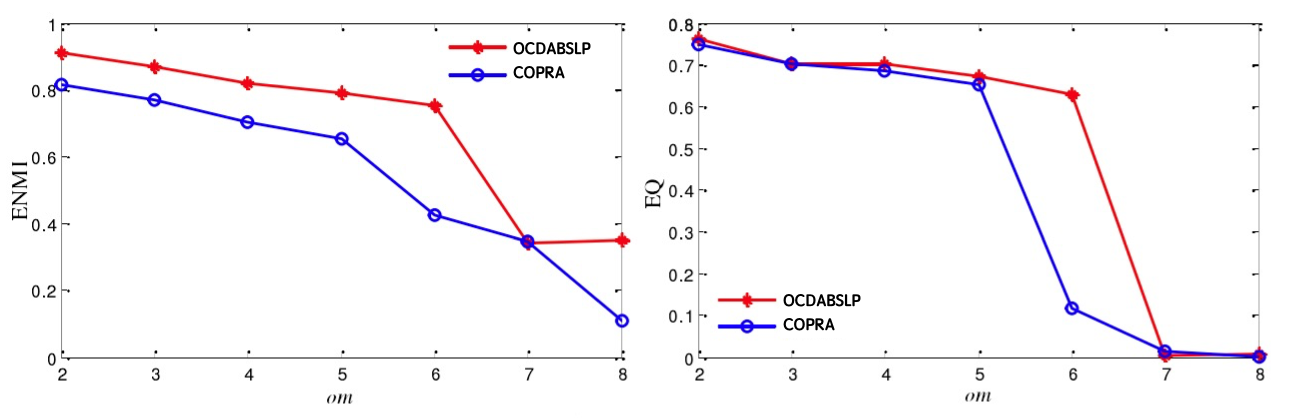
\includegraphics[width=0.75\textwidth]{figures/S7ENMI}
  \caption{N7网络上实验结果的ENMI和EQ比较}\label{fig:S7ENMI}

  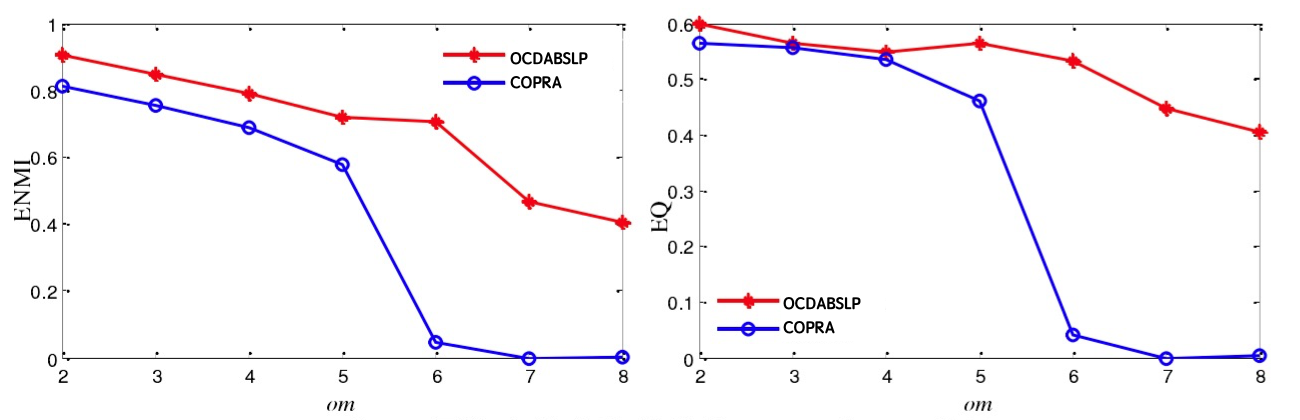
\includegraphics[width=0.75\textwidth]{figures/S8ENMI}
  \caption{N8网络上实验结果的ENMI和EQ比较}\label{fig:S8ENMI}

  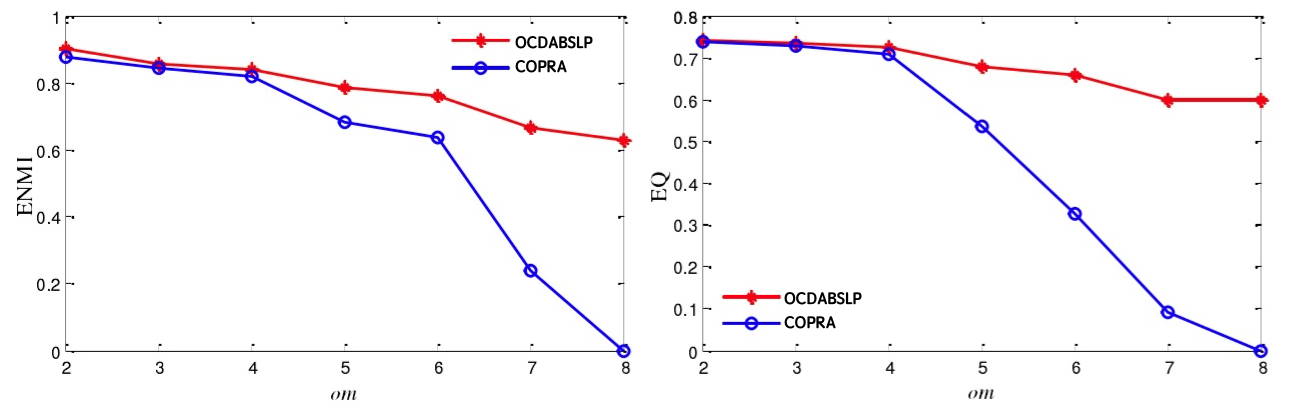
\includegraphics[width=0.75\textwidth]{figures/S9ENMI}
  \caption{N9网络上实验结果的ENMI和EQ比较}\label{fig:S9ENMI}

  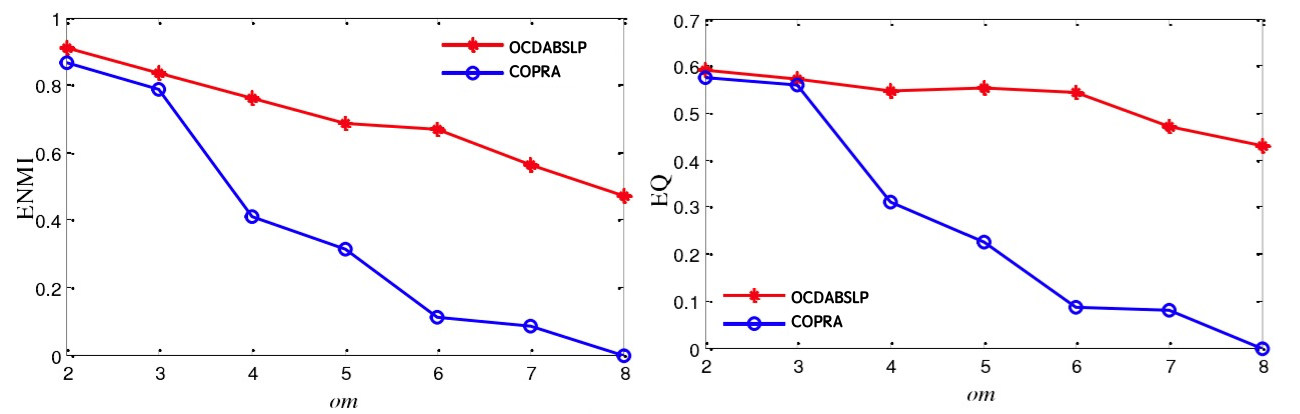
\includegraphics[width=0.75\textwidth]{figures/S10ENMI}
  \caption{N10网络上实验结果的ENMI和EQ比较}\label{fig:S10ENMI}

\end{figure}

从图\ref{fig:S7ENMI}$\sim$\ref{fig:S10ENMI}中可以明显的看出,ODABSLP算法的曲线基本都在COPRA算法曲线之上,且当om值较大时,ODABSLP算法的ENMI值和EQ值的大小都超出COPRA算法很多,这表明ODABSLP算法在实验效果上胜于COPRA算法。尤其是在节点能够属于大于5个社区的情况下,COPRA算法已经无法很好的进行重叠社区发现,图中COPRA算法曲线在om大于5时,有很明显的下滑趋势。而OCDABSLP算法的曲线整体较为平缓,表明om的大小并没有对算法实验效果造成较大的影响。

综上所述,OCDABSLP算法能够对具有重叠社区结构的社交网络进行高质量的重叠社区发现,且保持良好的稳定性。

% 从图\ref{fig:S7ENMI}$\sim$\ref{fig:S10ENMI}中可以看出,ODABSLP 算法不仅能够得到稳定的社区发现结果,而且得到的社区结构 ENMI 和 EQ 两个指标都优于 COPRA 算法。验证了本章所提方法在重叠社区发现方面能得到比较好的结果。

% (2)可视化对比

% 待加入。。。


% \subsection{实验总结}

% OCDABSLP 算法采用同步更新策略,在标签更新过程中,当一个节点拥有
% 的所有标签对应的隶属度都小于 1/v,且此时有多个标签的隶属度同时取最大值
% 时,将节点影响值引入到标签隶属度计算公式中,得到这些标签的影响强度,保
% 留影响强度最大的标签,取代传统 COPRA 算法随机保留其中一个标签的方法,
% 提高算法的稳定性。在重叠 LFR 数据集上的实验结果表明 OCDABSLP 算法解决
% 了 COPRA 算法不稳定的问题,能够检测得到较优的重叠社区结构,验证了本章
% 提出的稳定策略在重叠社区发现算法 COPRA 算法中的适用性。

\section{本章小结}

本章主要介绍了一种基于稳定标签传播的重叠社区发现算法,简称OCDABSLP。在简单分析了原始COPRA算法存在的缺陷之后,针对相应的缺陷介绍了稳定性解决方案。OCDABSLP算法采用了同步更新标签的策略,这点与CDABSLP算法不同;在标签选择方式上,对于邻居节点标签隶属度均小于既定阈值,且含有多个不同的最大隶属度标签的时候,选择最大隶属度标签中标签影响力模型计算值最大的那一个进行更新。在算法最终收敛之后,根据每个节点含有的标签将其划分到相应的社区,含有多个标签的节点即对应着存在于多个社区的重叠节点。通过真实网络以及人工网络中的验证实验,可知CDABSLP算法在具有良好的稳定性的同时兼具较高的运行效率,在多个评价指标之上社区发现准确率均有不错的表现。

% 本章主要介绍了一种基于稳定标签传播的重叠社区发现算法,简称OCDABSLP。OCDABSLP 算法采用同步更新策略,在标签更新过程中,当一个节点拥有
% 的所有标签对应的隶属度都小于 1/v,且此时有多个标签的隶属度同时取最大值
% 时,将节点影响值引入到标签隶属度计算公式中,得到这些标签的影响强度,保
% 留影响强度最大的标签,取代传统 COPRA 算法随机保留其中一个标签的方法,
% 提高算法的稳定性。在重叠 LFR 数据集上的实验结果表明 OCDABSLP 算法解决
% 了 COPRA 算法不稳定的问题,能够检测得到较优的重叠社区结构,验证了本章
% 提出的稳定策略在重叠社区发现算法 COPRA 算法中的适用性。
% %%==================================================
%% chapter05.tex for BIT Master Thesis
%% modified by 朱杰
%%==================================================
\chapter{社区发现算法相关实验与分析}
本章主要内容为本文提出的两种社区发现算法CDABSLP算法和OCDABSLP算法与其他相关算法的对比实验分析。首先介绍实验软硬件环境和采用的数据集,然后对算法的评价指标进行简单阐述,最后是相关对比实验的结果展示与分析。

\section{实验环境}

\subsection{实验硬件环境}
本文实现的CDABSLP算法和OCDABSLP算法所使用的机器配置如表\ref{tab:tab5-1}所示。

\begin{table}
  \centering
  \caption{计算机硬件配置} \label{tab:tab5-1}
  \begin{tabular*}{0.9\textwidth}{@{\extracolsep{\fill}}cccc}
  \toprule
    处理器			&2.2GHz 双核 Intel Core i7 \\
    内存容量			&8 GB 1600 MHz DDR3 \\
    硬盘容量			&128GB 固态硬盘 \\
  \bottomrule
  \end{tabular*}
\end{table}

\subsection{实验软件环境}
本文实现的CDABSLP算法和OCDABSLP算法使用Python语言编程实现,均基于Python的复杂网络相关软件包Networkx,使用Anaconda来对软件包进行管理和部署,具体配置如表\ref{tab:tab5-2}所示。

\begin{table}
  \centering
  \caption{计算机软件配置} \label{tab:tab5-2}
  \begin{tabular*}{0.9\textwidth}{@{\extracolsep{\fill}}cccc}
  \toprule
    操作系统			&macOS Sierra 10.12.6\\
    Anaconda版本  &conda 4.3.30 \\
    Networkx版本	&2.1 \\
    Python版本    &2.7.14\\
    Matplotlib版本  &2.0.2\\
    Numpy版本     &1.13.1\\
  \bottomrule
  \end{tabular*}
\end{table}

\section{数据集}
选用5个不同的真实数据集和LFR基准网络人工生成数据集进行实验验证本文所提算法的有效性。 


\subsection{真实数据集}
在5个常用的真实网络数据集上进行实验验证本章算法的有效性,这5个真
实网络数据集包括Karate、Dolphins 和 Football 等,各个数据集的详细信息如表\ref{tab:tab5-3}所示;

Karate是 Zachary 空手道俱乐部成员关系网络,网络中的所有节点对应各个成员,边表示两个端点对应的成员是好朋友。网络包含 34 个节点,78 条边和两个社区。 

Dolphins是 Lusseau 等人对栖息在新西兰 Doubtful Sound 峡湾的一
个宽吻海豚群体进行长达 7 年的观察所构造出的海豚关系网,该群体包含 2 个家族共 62 只宽吻海豚。由这个群里的所有成员及它们间的接触关系构成一个包含
62 个节点,159 条边和两个社区的网络。

Polbooks是从 Amazon 的图书销售记录抽象得到的网络数据集,
分析了 105 本与美国政治相关的书和它们的 441 条共同销售关系,依据亚马逊上
对图书的观点和评价情况,将这些书分为“自由派”、“中间派”和“保守派”三
个类。因此,此数据集包含 105 个节点,441 条边和三个社区。

Football是分析美国高校橄榄球比赛对阵表得到的数据集。共有 115
所高校派出代表队参赛,共进行了 616 场比赛,按各代表队地区的不同将这个包
含 115 个节点 616 条边的网络分为 12 个社区。 

Email是由 Guimer 等人收集公布的,包含位于西班牙加泰罗尼亚
自治区的罗维拉-威尔吉利大学(简称 URV)的教师和研究生之间的邮件往来关
系。两个用户或者说两个邮箱地址如果互相发送过邮件,就构成一条边。网络包
含 1133 个节点和 5451 条边。

\begin{table}
  \centering
  \caption{真实网络数据集} \label{tab:tab5-3}
  \begin{tabular*}{0.9\textwidth}{@{\extracolsep{\fill}}cccc}
  \toprule
    数据集名称		&节点数   &边数   &社区数\\
  \midrule
    Karate  &34 &78 &2\\
    Dolphins	&62 &159  &2\\
    Polbooks  &105  &441  &3\\
    Football  &115  &616  &12\\
    Email     &1133 &5451 \\
  \bottomrule
  \end{tabular*}
\end{table}

\subsection{LFR人工基准网络}
LFR基准网络是目前在社区发现领域使用最多的人工数据集之一。通
过调整网络生成参数可以产生用户需要的不同的人工数据集,LFR 基准网络的主
要生成参数及其含义如表\ref{tab:tab5-4}所示。

\begin{table}
  \centering
  \caption{LFR基准网络生成参数及其含义} \label{tab:tab5-4}
  \begin{tabular*}{0.9\textwidth}{@{\extracolsep{\fill}}cccc}
  \toprule
    参数		&含义\\
  \midrule
    N  &节点数\\
    avgk	&节点平均度\\ 
    maxk  &节点最大度\\
    mu  &网络拓扑结构混合参数\\
    minc  &最小社区规模\\
    maxc  &最大社区规模 \\
    on    &重叠节点个数\\
    om    &重叠节点可属于的社区个数\\
  \bottomrule
  \end{tabular*}
\end{table}

在 LFR 模型众多的生成参数中,混合参数$ mu \in [0,1]$是非常重要的一个参数,
mu 越小,说明连接社区之间的边越少,社区之间越“分离”,社区划分的难度随
着 mu 的增长而增大。on 和 om 两个参数用于生成具有重叠社区的数据集,生成
具有非重叠社区结构的数据集时,只需将 on 设置为 0,om 设置为 1 即可。 
生成六组具有非重叠社区结构的 LFR 基准网络数据集,所有的网络共享的
相同参数是 maxk = 50、on = 0 和 om = 1。每组包含九个 mu 值不同的数据集,分
别为 0.1 到 0.9,每组中的九个数据集共享参数 N、avgk、minc 和 maxc。其他参
数都取默认值。表\ref{tab:tab5-5}展示了这六组网络详细的生成参数情况。 

\begin{table}
  \centering
  \caption{六组LFR基准网络生成参数} \label{tab:tab5-5}
  \begin{tabular*}{0.9\textwidth}{@{\extracolsep{\fill}}ccccccc}
  \toprule
    编号		&N  &avgk &maxk &minc &maxc &mu\\
  \midrule
    1	&1000  &10 &50 &10 &50 &0.1~0.9\\
    2 &1000  &10 &50 &20 &100 &0.1~0.9\\
    3 &5000  &10 &50 &10 &50 &0.1~0.9\\
    4 &5000  &10 &50 &20 &100 &0.1~0.9\\
    5 &1000  &20 &50 &10 &50 &0.1~0.9\\
    6 &1000  &20 &50 &20 &100 &0.1~0.9\\
  \bottomrule
  \end{tabular*}
\end{table}

再生成四组具有重叠社区结构的 LFR 基准网络数据集,详细的生成参数如
表\ref{tab:tab5-6}示。 

\begin{table}
  \centering
  \caption{四组重叠LFR基准网络生成参数} \label{tab:tab5-6}
  \begin{tabular*}{0.9\textwidth}{@{\extracolsep{\fill}}ccccccccc}
  \toprule
    编号		&N  &avgk &maxk &minc &maxc &mu &on &om\\
  \midrule
    7	&1000  &15 &50 &10 &50 &0.1 &100 &2~8\\
    8 &1000  &15 &50 &10 &50 &0.3 &100 &2~8\\
    9 &5000  &15 &50 &20 &100 &0.1 &100 &2~8\\
    10 &5000  &15 &50 &20 &100 &0.3 &100 &2~8\\
  \bottomrule
  \end{tabular*}
\end{table}

\section{算法评价指标}
迄今为止,出现了各种各样的社区发现算法,如何评价不同的的发现算法的好坏是一个非常重要的问题。为此,学者们提出了多种社区结构评价指标用来评价网络社区划分质量,其中比较有代表性的有模块度、NMI等。下面介绍这些指标。

\subsection{模块度}
模块度是目前学者们最常用和经典的网络社区结构评价指标,它最初是被Newman等人于2004年提出来的\cite{2002Community}。其通过比较现有网络和基准网络在相同社区划分下的连接密度差来衡量网络社区的优劣,其中基准网络是由原网络具有相同度序列的随机网络。模块度计算方式详见公式\ref{eqn:modular}。

\begin{equation}
  \label{eqn:modular}
  Q=\frac{1}{2m}\sum_{i,j}\left [ A_{ij}-\frac{k_ik_j}{2m} \right ]\delta (c_i, c_j)  
\end{equation}

其中,A 表示网络中的邻接矩阵, m 表示网络中边的总数,$k_i$和$k_j$表示节点 i 和 j 的度数,$c_i$和$c_j$表示节点 i 和 j 所属的社区。如果$i=j,\delta(c_i,c_j)=1$,反之$\delta(c_i,c_j)=0$

重叠社区模块度可以在此基础上修改为\ref{eqn:modular2}。

\begin{equation}
  \label{eqn:modular2}
  Q=\frac{1}{2m} \sum_{k=1}^c \sum_{i,j \in C_k} \frac{1}{O_iO_j} \left [ A_{ij}-\frac{k_ik_j}{2m} \right ]  
\end{equation}

在公式\ref{eqn:modular2}中,i和j表示网络中的两个节点,m表示网络中边的数量,$k_i$和$k_j$表示节点i和j的度数,$O_i$和$O_j$表示节点i和j所属的社区的个数,A表示网络的邻居矩阵,$C_k$表示网络的第k个社区。该公式的数学意义为:网络中同一社区内部的边的比例与在同样社区结构下的基准网络内部边的比例的期望值之差。模块度越高,则网络中社区划分结果越好。

\subsection{NMI}
随着在线社交网络的发展,人们发现在线社交网络的很多数据中存在着暗示各个节点的社区属性信息。例如,在人人网的学校信息便揭示了网络节点中属于同一学校的社区结构,Facebook中的兴趣信息同样表征了具有相同兴趣的虚拟用户群体。这些数据在为社区发现问题提供了丰富的信息的同时,也在一定程度上为虚拟社区结构优劣的评判提供了标准答案。针对这种预先拥有一定虚拟社区结构信息的情况下,Leon Danon等人【34】提出了Normalized Mutual Information(NMI)利用信息化熵来衡量算法划分的社区结构和预先已知的社区结构之间的差异。NMI是基于混合矩阵(Confusion Matrix)N来计算的数字指标。NMI计算方式详见公式\ref{eqn:nmi}。

\begin{equation}
  \label{eqn:nmi}
  NMI=\frac{ -2 \sum_{i,j} N_{ij}  ln{\frac{N_{ij}}{N_iN_j}} } {\sum_{i}N_iln{\frac{N_i}{n}}+\sum_{j}N_jln{\frac{N_j}{n}}}
\end{equation}

使用该数字指标,可以衡量划分出来的社区结构与已知的网络社区结构的差异程度值,该值越大,则表明获得的社区结构划分越好,当该值达到最大化值1时,说明算法发现的社区结构与已知社区结构完全已知,效果最好。

\begin{figure}
 \centering
 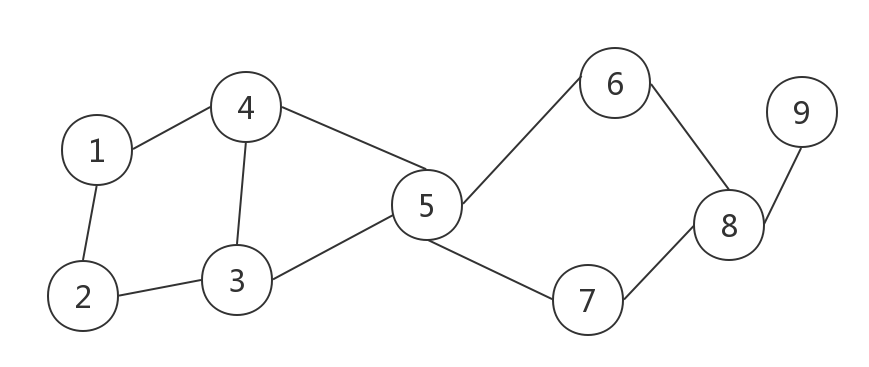
\includegraphics[width=0.75\textwidth]{figures/fig5-1}
 \caption{NMI网络示例图}\label{fig:fig5-1}
\end{figure}

下面以图\ref{fig:fig5-1}为例来说明计算NMI的过程。假设已知的最佳社区结构划分为集合{1,2,3,4}和{5,6,7,8},相应的社区划分向量表示为a = (1,1,1,1,2,3,3,3,3),再假设某算法获得的社区划分结构可以用向量表示为b = (3,3,3,3,2,1,1,1,1)来表示。根据已知的社区划分向量,可以构造混合矩阵\ref{eqn:n}。

\begin{equation}
  \label{eqn:n}
  N=\begin{bmatrix}
    0 & 0 &4 \\ 
    0 & 1 & 0\\ 
    4 & 0 & 0
    \end{bmatrix}
\end{equation}

根据上式计算可知,该划分的NMI值为1。

\section{实验对比}

% \subsection{模块度的对比}
% 暂时凑字数

% \subsection{模块度的对比}
% 暂时凑字数
% \subsection{模块度的对比}
% 暂时凑字数
% \subsection{模块度的对比}
% 暂时凑字数
% \subsection{可视化对比}
% 暂时凑字数
\section{实验总结}
% 暂时凑字数



%%==================================================
%% conclusion.tex for BIT Master Thesis
%% modified by 朱杰
%%==================================================


\begin{conclusion}

本文采用……。{\color{blue}(结论作为学位论文正文的最后部分单独排写,但不加章号。结论是对整个论文主要结果的总结。在结论中应明确指出本研究的创新点,对其应用前景和社会、经济价值等加以预测和评价,并指出今后进一步在本研究方向进行研究工作的展望与设想。结论部分的撰写应简明扼要,突出创新性。)}

\end{conclusion}

%% 参考文献,五号字,使用 BibTeX,包含参考文献文件.bib

%\bibliography{reference/chap1,reference/chap2} %多个章节的参考文献
\bibliography{reference/chapter1,reference/chapter2,reference/chapter3,reference/chapter4}


%%%%%%%%%%%%%%%%%%%%%%%%%%%%%%
%% 后置部分
%%%%%%%%%%%%%%%%%%%%%%%%%%%%%%

%% 附录(章节编号重新计算,使用字母进行编号)
% \appendix
% \renewcommand\theequation{\Alph{chapter}--\arabic{equation}}  % 附录中编号形式是"A-1"的样子
% \renewcommand\thefigure{\Alph{chapter}--\arabic{figure}}
% \renewcommand\thetable{\Alph{chapter}--\arabic{table}}

% %%==================================================
%% app1.tex for BIT Master Thesis
%% modified by yang yating
%% version: 0.1
%% last update: Dec 25th, 2016
%%==================================================


\chapter{***}

附录相关内容…
 
% 
\chapter{Maxwell Equations}


因为在柱坐标系下,$\overline{\overline\mu}$是对角的,所以Maxwell方程组中电场$\bf
E$的旋度

所以$\bf H$的各个分量可以写为:
\begin{subequations}
  \begin{eqnarray}
    H_r=\frac{1}{\mathbf{i}\omega\mu_r}\frac{1}{r}\frac{\partial
      E_z}{\partial\theta } \\
    H_\theta=-\frac{1}{\mathbf{i}\omega\mu_\theta}\frac{\partial E_z}{\partial r}
  \end{eqnarray}
\end{subequations}
同样地,在柱坐标系下,$\overline{\overline\epsilon}$是对角的,所以Maxwell方程组中磁场$\bf
H$的旋度
\begin{subequations}
  \begin{eqnarray}
    &&\nabla\times{\bf H}=-\mathbf{i}\omega{\bf D}\\
    &&\left[\frac{1}{r}\frac{\partial}{\partial
        r}(rH_\theta)-\frac{1}{r}\frac{\partial
        H_r}{\partial\theta}\right]{\hat{\bf
        z}}=-\mathbf{i}\omega{\overline{\overline\epsilon}}{\bf
      E}=-\mathbf{i}\omega\epsilon_zE_z{\hat{\bf z}} \\
    &&\frac{1}{r}\frac{\partial}{\partial
      r}(rH_\theta)-\frac{1}{r}\frac{\partial
      H_r}{\partial\theta}=-\mathbf{i}\omega\epsilon_zE_z
  \end{eqnarray}
\end{subequations}
由此我们可以得到关于$E_z$的波函数方程:
\begin{eqnarray}
  \frac{1}{\mu_\theta\epsilon_z}\frac{1}{r}\frac{\partial}{\partial r}
  \left(r\frac{\partial E_z}{\partial r}\right)+
  \frac{1}{\mu_r\epsilon_z}\frac{1}{r^2}\frac{\partial^2E_z}{\partial\theta^2}
  +\omega^2 E_z=0
\end{eqnarray}
 

%(其后部分无编号)
\backmatter

% 发表文章目录
% %%==================================================
%% pub.tex for BIT Master Thesis
%% modified by yang yating
%% version: 0.1
%% last update: Dec 25th, 2016
%%==================================================

\begin{publications}{99}

    \item\textsc{高凌}. {交联型与线形水性聚氨酯的形状记忆性能比较}[J].
      化工进展, 2006, 532-535.(核心期刊)
    
\end{publications}

% 致谢
% %%==================================================
%% thanks.tex for BIT Master Thesis
%% modified by 朱杰
%%==================================================

\begin{thanks}

光阴荏苒,岁月如梭,两年的研究生生活转瞬即逝。值此毕业论文即将完稿之际,我对帮助过我的老师、同学以及亲友表达由衷的感谢,并对本硕共培养了我6年的母校北京理工大学致以诚挚的敬意。

首先感谢我的两位导师:讲师张欣和副教授金福生。张老师是我名义上的导师,但是实际上两年研究生生涯我接触更多的是金老师。在参与金老师负责的实验室所承接的项目的工作中,我积累到了宝贵的项目经验。本论文的工作也包含了金老师悉心的监督和指导,在论文的撰写上提出了很多宝贵意见。感谢两位导师的帮助和指导。

感谢陪伴我两年的舍友张俊逸、谢辰和刘哲湘。两年的朝夕相处与你们建立了深厚的情谊,不论是学习还是生活中都少不了你们的帮助和支持。看着你们如今都找到满意的工作,有了很好的归宿,真心替你们开心,这一毕业就是各奔东西了,祝大家都前程似锦吧。

感谢我的同窗们李璟明、蔡天倚、王宇侠等,感谢帮助过我的学长学姐龚思胜、朱冲冲、孙晨光等,感谢你们对我学习生活上的帮助和支持。

%感谢两位前女友伴我度过了这虽有瑕疵但值得回味的研究生两年。FC,是你的鼓励和陪伴,才使得我更加努力积极的找到了现在的工作,谢谢你,也祝你万事胜意。

感谢我的父母和家人,是他们无私的关怀和奉献支撑我完成了学业。

最后,感谢各位参加论文评审和论文答辩的老师们的批评与指导!
\end{thanks}

% 作者简介(博士论文需要)
% %%==================================================
%% resume.tex for BIT Master Thesis
%% modified by yang yating
%% version: 0.1
%% last update: Dec 25th, 2016
%%==================================================

\begin{resume}

本人…。

\end{resume}



\end{document}
